\documentclass[12pt,openright,oneside,a4paper,english,french,spanish]{abntex2}

\usepackage{cmap}	
\usepackage{lmodern}	
\usepackage[T1]{fontenc}	
\usepackage[utf8]{inputenc}		
\usepackage{lastpage}		
\usepackage{indentfirst}
\usepackage{color}	
\usepackage{graphicx}	
\usepackage{units}
\usepackage[brazilian,hyperpageref]{backref}
\usepackage[alf]{abntex2cite}
\usepackage{bold-extra}
\usepackage{eso-pic}
\usepackage{pdflscape}
\usepackage{tabu}
\usepackage{graphicx}
\usepackage[table,xcdraw]{xcolor}
\usepackage{multirow}
\usepackage{float}
\usepackage{xspace}
\usepackage[ruled,linesnumbered]{algorithm2e}
\usepackage{pdfpages}
% \usepackage{tabularx}
% \usepackage{booktabs}

\usepackage{booktabs,makecell,tabularx}
\usepackage{siunitx}
\usepackage{adjustbox}
\usepackage{array,booktabs}
\newcolumntype{C}[1]{>{\centering\arraybackslash}p{#1}}
\renewcommand\theadfont{\small}
\newcolumntype{L}{>{\raggedright\arraybackslash}X}

\newcommand{\itractool}{DTEST\xspace}

%Comandos para revisão
\newcommand{\rev}[1]{{\color{green}#1}\xspace}
\newcommand{\del}[1]{{\color{red}#1}\xspace}

%Comandos para impedir linhas órfãs e viúvas
\clubpenalty=10000
\widowpenalty=10000

\renewcommand{\backrefpagesname}{Citado na(s) página(s):~}
\renewcommand{\backref}{}
\renewcommand*{\backrefalt}[4]{
	\ifcase #1 %
		Nenhuma citação no texto.%
	\or
		Citado na página #2.%
	\else
		Citado #1 vezes nas páginas #2.%
	\fi}%
% ---


\usepackage{fixos/customizacoes}

% Dados pessoais
\autor{Letícia de Souza Santos}
\curso{Engenharia de Software}

% Dados do trabalho
\titulo{Sistema de Recomendação para Atribuição de Tarefas de Testes Baseado em Perfil de Testadores }
\data{2019}
\palavraChaveUm{}
\palavraChaveDois{}

% Dados da orientacao
\orientador{Profa. Dra. Rejane Maria da Costa Figueiredo}
\coorientador{Prof. Dr. Auri Marcelo Rizzo Vincenzi}

% Dados para a ficha catalográfica
\cdu{02:141:005.6}

% Dados da aprovação do trabalho
\dataDaAprovacao{junho de 2019}
\membroConvidadoUm{Prof. Ms. Ricardo Ajax Dias Kosloski}
\membroConvidadoDois{Prof. Dr. Glauco Vitor Pedrosa}

\local{Brasília, DF}
\instituicao{%
  Universidade de Brasília -- UnB
  \par
  Faculdade UnB Gama -- FGA
}
\tipotrabalho{Trabalho de Conclusão de Curso}
\preambulo{Monografia submetida ao curso de graduação em \imprimircurso\ 
da Universidade de Brasília, como requisito parcial para obtenção do Título 
de Bacharel em \imprimircurso.}

\definecolor{blue}{RGB}{41,5,195}
\makeatletter
\hypersetup{
     	%pagebackref=true,
		pdftitle={\@title}, 
		pdfauthor={\@author},
    	pdfsubject={\imprimirpreambulo},
	    pdfcreator={LaTeX with abnTeX2},
		pdfkeywords={abnt}{latex}{abntex}{abntex2}{trabalho acadêmico}, 
		colorlinks=true,       		% false: boxed links; true: colored links
    	linkcolor=blue,          	% color of internal links
    	citecolor=blue,        		% color of links to bibliography
    	filecolor=magenta,      		% color of file links
		urlcolor=blue,
		bookmarksdepth=4
}
\makeatother
\setlength{\parindent}{1.3cm}
\setlength{\parskip}{0.2cm}  
\makeindex


\begin{document}

\frenchspacing 
\imprimircapa
\imprimirfolhaderosto*

\begin{fichacatalografica}
	\vspace*{\fill}					% Posição vertical
	\hrule							% Linha horizontal
	\begin{center}					% Minipage Centralizado
	\begin{minipage}[c]{12.5cm}		% Largura
	
	\imprimirautor
	
	\hspace{0.5cm} \imprimirtitulo  / \imprimirautor. --
	\imprimirlocal, \imprimirdata-
	
	\hspace{0.5cm} \pageref{LastPage} p. : il. (algumas color.) ; 30 cm.\\
	
	\hspace{0.5cm} \imprimirorientadorRotulo~\imprimirorientador\\
	
	\hspace{0.5cm}
	\parbox[t]{\textwidth}{\imprimirtipotrabalho~--~\imprimirinstituicao,
	\imprimirdata.}\\
	
	\hspace{0.5cm}
		1. \imprimirpalavrachaveum.
		2. \imprimirpalavrachavedois.
		I. \imprimirorientador.
		II. Universidade de Brasília.
		III. Faculdade UnB Gama.
		IV. \imprimirtitulo\\ 			
	
	\hspace{8.75cm} CDU \nomecdu\\
	
	\end{minipage}
	\end{center}
	\hrule
\end{fichacatalografica}

% \input{editaveis/errata}
\begin{folhadeaprovacao}

  \begin{center}
    {\ABNTEXchapterfont\large\imprimirautor}

    \vspace*{\fill}\vspace*{\fill}
    {\ABNTEXchapterfont\bfseries\Large\imprimirtitulo}
    \vspace*{\fill}

    \hspace{.45\textwidth}
    \begin{minipage}{.5\textwidth}
        \imprimirpreambulo
    \end{minipage}%
    \vspace*{\fill}
   \end{center}

   Trabalho aprovado. \imprimirlocal, \imprimirdatadaaprovacao:

   \assinatura{\textbf{\imprimirorientador} \\ Orientadora}
   \assinatura{\textbf{Prof. Dr. Auri Marcelo Rizzo Vincenzi} \\ Coorientador}
   \assinatura{\textbf{\imprimirmembroconvidadoum} \\ Convidado 1}
  \assinatura{\textbf{\imprimirmembroconvidadodois} \\ Convidado 2}
  

   \begin{center}
    \vspace*{0.5cm}
    {\large\imprimirlocal}
    \par
    {\large\imprimirdata}
    \vspace*{1cm}
  \end{center}

\end{folhadeaprovacao}

% \input{editaveis/dedicatoria}
\begin{agradecimentos}

Aos meus pais, pelo cuidado e amor dedicados a mim. Ao meu irmão, Vitor, por me alegrar e me encher de carinho, mesmo em momentos de estresse. À minha irmã, Laíse, pelo apoio e por me presentear com um dos motivos da minha persistência, minha sobrinha, Cecília.

À professora Rejane Figueiredo, pelas oportunidades, pela orientação e incentivo que oferece à minha carreira acadêmica. Ao professor Auri Vincenzi, pela coorientação e pela oportunidade de trabalharmos juntos, ainda que a 963 km de distância.

Aos professores Milene Serrano e Maurício Serrano, por me impulsionarem, através do PIBIC, ainda no ensino médio, a ingressar na Engenharia, ainda que muitos ao meu redor dissessem que a área não era para mim.

À professora Cristiane Soares Ramos, pelos ensinamentos e abraço acolhedor em um dos momentos mais difíceis da minha graduação. 

Ao meu namorado, Rafael Fazzolino, pelo incentivo em ampliar meus saberes intelectuais, pela paciência, companheirismo e tamanho afeto.

Por fim, agradeço a todas as mulheres da minha vida, que estiveram comigo na luta comum das que tentam acertar e se superar, pela empatia e desejo de tornar o mundo um lugar mais congruente. 

\end{agradecimentos}

\begin{epigrafe}
    \vspace*{\fill}
 	\begin{flushright}

		\textit{"Todas nós seguimos em frente quando percebemos\\ como são fortes e admiráveis as mulheres à nossa volta."\\
		(Rupi Kaur)}
	\end{flushright}
\end{epigrafe}

\begin{resumo}

A Universidade de Brasília (UnB), por meio do \textit{Information Tech-nology Research and Application Center} (ITRAC), em parceria com o Ministério da Economia (ME), tem contribuído com o Governo Federal Brasileiro para a transformação de serviços públicos em serviços digitais. O ITRAC definiu um processo de validação sistematizado com o intuito de garantir a qualidade destes serviços, a partir da utilização dos Testes Exploratórios, com a Metáfora do Turista, que dependem da personalidade e conhecimento dos envolvidos na atividade de teste. Dessa forma, supõe-se que o perfil do testador tenha algum impacto na aplicação das \textit{tours} utilizadas na metáfora do turista. Neste trabalho propõe-se a obtenção de perfis de testadores, utilizando características pessoais e experiência do domínio para Atribuição automática de atividades de teste, a partir do desenvolvimento de um sistema de recomendação, utilizando a equipe de testadores do ITRAC. O principal procedimento técnico escolhido para esta avaliação foi a Pesquisa-Ação, comumente utilizada na resolução de problemas coletivos, envolvendo pesquisadores e participantes de modo cooperativo. A primeira etapa desta metodologia, o Diagnóstico, foi realizado para compreensão do objeto de estudo, enquanto que as três últimas etapas, o Planejamento, a Ação e a Avaliação serão levadas em consideração para a construção de instrumentos em ciclos de interação com a equipe, afim de facilitar o entendimento sobre o funcionamento do módulo da ferramenta proposta.

% \del{alterei o ``propomos'' por ``propõe-se'' para deixar no impessoal.}
 \vspace{\onelineskip}

 \noindent
 \textbf{Palavras-chave}: Sistema de Recomendação. Testes Exploratórios. Perfil de Testadores.
\end{resumo}

\begin{resumo}[Abstract]
 \begin{otherlanguage*}{english}
   The University of Brasília (UnB), through the Information Technology Research and Application Center (ITRAC), in partnership with the Ministry of Economy (ME), has contributed with the Brazilian Federal Government for the transformation of services public services in digital services. The ITRAC defined a systematized validation process with the purpose of guaranteeing the quality of these services, based on the use of the Exploratory Tests, with the Tourist Metaphor, which depends on the personality and knowledge of those involved in the test activity. Thus, it is assumed that the tester profile has some impact on the application of the \ textit {tours} used in the tourist metaphor. In this work, we propose to obtain profiles of testers, using personal characteristics and domain experience for automatic assignment of test activities, from the development of a recommendation system, using the team of ITRAC testers. The main technical procedure chosen for this evaluation was Research-Action, commonly used in solving collective problems, involving researchers and participants in a cooperative way. The first stage of this methodology, the Diagnosis, was carried out to understand the object of study, while the last three steps, Planning, Action, and Evaluation will be taken into account for the construction of instruments in cycles of interaction with the team, in order to facilitate the understanding of the operation of the module of the proposed tool.

   \vspace{\onelineskip}

   \noindent
   \textbf{Key-words}: System of Recommendation. Exploratory Testing. Profile of Testers.
 \end{otherlanguage*}
\end{resumo}

\pdfbookmark[0]{\listfigurename}{lof}
\listoffigures*
\cleardoublepage
\pdfbookmark[0]{\listtablename}{lot}
\listoftables*
\cleardoublepage

\begin{siglas}

    \item[APF] Administração Pública Federal
    \item[DTEST] Digital Transformation Environment Support Tool
    \item[EGD] Estratégia de Governança Digital da Administração Pública Federal
    \item[ETAT] Teste de Aptidão de Teste Exploratório
    \item[EUD] End-user development
    \item[FBC] Filtragem Baseada em Conteúdo
    \item[FC] Filtragem Colaborativa
    \item[UnB] Universidade de Brasília
    \item[IA] Inteligência Artificial
    \item[ITRAC] Information Technology Research and Application Center
    \item[ME] Ministério da Economia
    \item[MP] Ministério do Planejamento Desenvolvimento e Gestão
    \item[OECD] Organisation for Economic Co-operation and Development (Organização
  para cooperação e desenvolvimento econômico)
    \item[SEI] Sistema Eletrônico de Informações
    \item[SMV] Serviço Mínimo Viável
    \item[SR] Sistema de Recomendação
    \item[SUT] Service Under Testing
    \item[TD]  Transformação Digital
    \item[TE] Teste Exploratório

\end{siglas}
\pdfbookmark[0]{\contentsname}{toc}
\tableofcontents*
\cleardoublepage


\textual

\chapter{Introdução}        
\label{ch:introducao}
% A atividade de teste é essencial dentro do contexto da Engenharia de Software objetivando a validação do comportamento
% do software e identificação de possíveis problemas de funcionamento. Nas últimas décadas, tem sido estabelecidas
% técnicas, critérios, métodos e ferramentas para a produção de software a fim de acompanhar a crescente utilização de
% sistemas por parte da maioria das práticas da atividade humana~\cite{maldonado2004introduccao}.
% Através da examinação diretamente do software em execução, o teste fornece um \textit{feedback} realista de seu comportamento,
% o que o torna o complemento inevitável de outras técnicas de análise e garantia de qualidade na indústria~\cite{bertolino2007software}.

    \section{Contexto}

O Governo Federal Brasileiro incentiva os órgãos públicos a transformarem seus serviços em serviços digitais. Algumas das iniciativas estão relacionadas à publicação de estratégias e decretos que buscam concretizar o uso de tecnologias digitais como uma estratégia de modernização de determinados setores. Alguns exemplos são: a criação de uma plataforma digital, a criação de um kit para transformação de serviços em serviços digitais, a oferta de uma solução tecnológica para a digitização de serviços, entre outros. 

Em 2017, o antigo Ministério do Planejamento, Gestão e Desenvolvimento (MP), atualmente compondo o Ministério da Economia (ME), lançou o programa de \textit{Transformação de Serviços Públicos} denominado \textit{Kit de Transformação}. O Kit é composto de seis fases independentes entre si: \textit{Questione}, \textit{Personalize}, \textit{Reinvente}, \textit{Facilite}, \textit{Integre} e \textit{Comunique}~\cite{BRASIL2017}. O principal objetivo do Kit é simplificar o acesso a determinados serviços e ofertas, a partir da perspectiva dos cidadãos e das empresas.

Nesse cenário, a Universidade de Brasília (UnB), por meio do \textit{Information Technology Research and Application Center} (ITRAC), laboratório que promove pesquisas e desenvolvimentos na área de TI, contribui com o Ministério da Economia (ME) no apoio ao Kit de Transformação. A parceria entre as duas instituições envolve a definição de um processo de transformação de serviços públicos, com a inserção de atividades de desenvolvimento e de qualidade de software.

O presente trabalho está relacionado à fase \textit{Facilite}. Essa fase provê recursos e ferramentas para apoiar os órgãos federais a simplificar e digitizar seus serviços a partir de uma solução tecnológica.

No ITRAC foi definido um processo de digitização de serviços governamentais, que faz uso de uma ferramenta baseada numa abordagem de \textit{meta-design}~\cite{fogli2012meta}, que utiliza modelagem de processos e configuração gráfica dos campos envolvidos para transformação dos serviços governamentais. Esta ferramenta foi adotada pelo ME, via terceirização, e possibilita um processo de desenvolvimento descentralizado que dá celeridade ao processo de transformação digital no governo brasileiro. O processo de transformação envolve o emprego de técnicas que vão desde a análise do serviço, passando por elicitação dos requisitos, mapeamento do processo envolvido no serviço analisado e construção do mesmo na ferramenta de \textit{meta-design}. O processo de transformação envolve, ainda, atividades de \textit{verificação} e \textit{validação} do serviço digitizado, buscando garantir a qualidade do produto que será entregue a população.

Para o processo de verificação e validação dos serviços transformados, as atividades de testes dependem fortemente dos requisitos dos serviços transformados. Contudo, muitas vezes, os requisitos inexistem ou estão instáveis, isso é, os requisitos fornecidos pelos órgãos não são concisos. 

A problemática de se testar sem requisitos está presente neste trabalho, visto que os serviços digitizados não possuem uma documentação formal de requisitos e o código-fonte não é acessível à equipe de teste, o que dificulta a extração de informações. Tais restrições são decorrentes da forma de contratação definida pelo ME, via licitação pública, na qual, a empresa terceirizada, não é obrigada a entregar a documentação, código-fonte, e os testes realizados durante o desenvolvimento do serviço digitizado. 

% \del{Não sei se isso é verdade. Se for, acho que vale a pena incluir}.

Segundo Barr et. al.,~\cite{barr2015oracle} requisitos instáveis ou inexistentes podem fazer com que os testadores se deparem com o Problema do Oráculo, ou seja, um cenário de difícil identificação do comportamento correto do serviço digitizado, dificultando a comparação entre o comportamento obtido e o comportamento esperado durante a execução dos casos de teste.

No ITRAC foi desenvolvido um processo de validação sistematizado, com o intuito de garantir a qualidade da digitização dos serviços. Dado que o código-fonte do serviço não está disponível, o processo emprega a técnica de Teste Exploratório, sugerido por~\cite{whittaker2009exploratory}. 

Essa abordagem possibilita que o testador não dependa de um conjunto de teste pré-projetados e utilize-se da Metáfora do Turista, também proposta por~\cite{whittaker2009exploratory}, como uma estratégia para guiar, a partir das chamadas \textit{``tours''}, a criação e execução dos casos de teste, facilitando, ainda, a extração de requisitos e regras de negócio a partir da exploração do software analisado.

Vale ressaltar que a utilização dos \textit{Testes Exploratórios}, com a  \textit{Metáfora do Turista}, depende da imaginação,  personalidade e conhecimento dos envolvidos na atividade de teste~\cite{itkonen2012role}. Isso se dá, devido ao quesito humano envolvido na atividade de Teste Exploratório, conforme destacado por~\cite{whittaker2009exploratory}.

Dessa forma, supõe-se que o perfil do testador tenha algum impacto na aplicação das \textit{tours} utilizadas na metáfora do turista proposta por~\cite{whittaker2009exploratory}, visto que os casos de teste gerados e suas sequências variam muito a depender do testador. O entendimento desse perfil e suas principais características podem trazer benefícios para a equipe de testes.

Entre os benefícios envolvidos, pode-se destacar a atividade de \textit{Atribuição de tarefas de teste para testadores.}
Normalmente, as tarefas de teste são alocados por gerentes para que sejam seguidas pelos testadores que estiverem disponíveis em determinado momento. Em vista disso, uma das formas de se maximizar a produtividade em uma equipe de testes é alocar tarefas de acordo com o perfil de testadores~\cite{miranda2012recommender}. Entretanto, a Atribuição de tarefas de forma manual não é trivial visto que, em grandes empresas, os gerentes de teste são responsáveis por alocar grande número de tarefas para vários testadores. No contexto do presente trabalho, as tarefas de teste a serem atribuídas dizem respeito aos tours do Teste Exploratório.

Um dos possíveis minimizadores desse desafio de atribuição de tours é o emprego dos sistemas de recomendação para alocar tarefas a perfis específicos baseado em análises de alocações anteriores, 
como mostram os trabalhos de~\cite{anvik2006should} e~\cite{miranda2012recommender}.

Esse novo  emprego dos sistemas de recomendação motiva este trabalho, visto que o desenvolvimento de um sistema de recomendação poderá auxiliar na \textit{atribuição de tours} para uma equipe de testadores, buscando maximizar a eficiência deles e contribuir com grandes equipes.

% Através do advento da evolução da tecnologia e expansão da internet surge a expressão \textit{Governo Digital},
% que se refere ao uso de tecnologias digitais como uma estratégia de modernização de um Governo, que adota a tecnologia
% da informação e comunicação (TIC) para prover serviços~\cite{fang2002government}. O termo \textit{e-Gov} surgiu no final da década de 1990 e cresceu a um tamanho considerável desde então. Nos últimos
% anos, deu origem a várias conferências de cunho científico, aumentando seu conteúdo e posição no que se refere a outros
% campos de pesquisa e disciplinas~\cite{gronlund2005introducing}.

% No Brasil, embora as medidas de modernização do setor público tenham começado a ser adotadas na década de 70, as ênfases se deram
% apenas com a crise fiscal dos anos 80, onde a intervenção estatal ficou conhecida como reforma da gestão pública que, aliada as
% TICs, proporcionou com que os governos no Brasil oferecessem serviços públicos eletrônicos à população no início da década de
% 2000~\cite{przeybilovicz2015desenvolvimento}.



% Em vista deste cenário de digitalização do serviço público, é de suma importância garantir a qualidade dos serviços digitalizados
% devido aos efeitos nos domínios nacionais e internacionais. De acordo com~\cite{myers2004art}, é preciso que as características
% dos projetos sejam levadas em consideração no momento de definição da estratégia de teste para assegurar que a verificação e
% a validação sejam economicamente viáveis, analisando a complexidade e quantidade de caminhos envolvidos para que se atinja a
% qualidade desejada.






    
    \section{Problema}

A criação de casos de teste por uma equipe pode implicar na produtividade a depender do nível de \textit{expertise} dos testadores. Isto é, a experiência dos testadores relacionados aos serviços a serem testados disponibilizados pode variar bastante, devido às variações de nível de escolaridade, experiência com testes, tipos de testes, técnicas já utilizadas, entre outras. 

No contexto atual do ME, a equipe de transformação de serviços não é volumosa o suficiente para reconhecer o perfil dos testadores e apoiar, como amostra, o desenvolvimento do sistema de recomendação de tours para teste de serviços digitizados. 

Sendo assim, a pergunta de pesquisa definida neste trabalho é:

% \del{Sistema de Recomendação para Atribuição de Tarefas de Testes Baseado em Perfil de Testadores}

\textit{``Como desenvolver um sistema de recomendação para atribuição de tarefas de testes baseado no perfil de testadores no contexto de digitalização de serviços públicos?''}


    \section{Objetivos}
\subsection{Objetivo Geral}

Desenvolver um sistema de recomendação para atribuição de atividades de teste baseado em perfil de testadores.

\subsection{Objetivos Específicos}

\begin{itemize}
		\item Definir um conjunto de pessoas como amostra para a definição de um sistema de recomendação;
 		\item Definir um processo de atribuição de atividades de testes adequada a perfis de testadores;
% 		\item Identificar o registro de atividades de teste realizadas por cada perfil gerado pela ferramenta ITRAC;
		\item Definir um processo de análise dos registros de testes realizados por cada perfil durante os ciclos de teste e
		\item Especificar um sistema de recomendação para atribuição de atividades de teste baseada em perfis. 
		
% \del{Eu colocaria essa como sendo o objetivo geral já que acho que apenas especificaremos o sistema no seu trabalho, correto? Não chegamos a desenvolver o sistema de recomendação.}

	\end{itemize}


    \section{Metodologia}

Dado o objetivo deste trabalho, a metodologia de pesquisa foi definida e classificada e um plano metodológico foi estruturado em fases e etapas.

Dado o contexto prático, no qual o objetivo é a criação de um módulo de uma ferramenta que promoverá a recomendação de \textit{tours} de Teste Exploratório baseado no perfil do testador, esta pesquisa é de natureza aplicada. A abordagem é qualitativa e quantitativa, uma vez que a análise dos dados será subjetiva, mas também fará uso de métodos e técnicas estatísticas.

Quanto ao tipo/objetivo, a pesquisa é classificada como explicativa, que possibilita a identificação de fatores que contribuem ou determinam a ocorrência de fenômenos, de modo a aprofundar o conhecimento da realidade e a explicar a razão e motivo das coisas~\cite{gil2002elaborar}. 

A Figura \ref{fig:classificacaoMetodologica}  apresenta esta classificação.

        \begin{figure}[h]
          \centering
          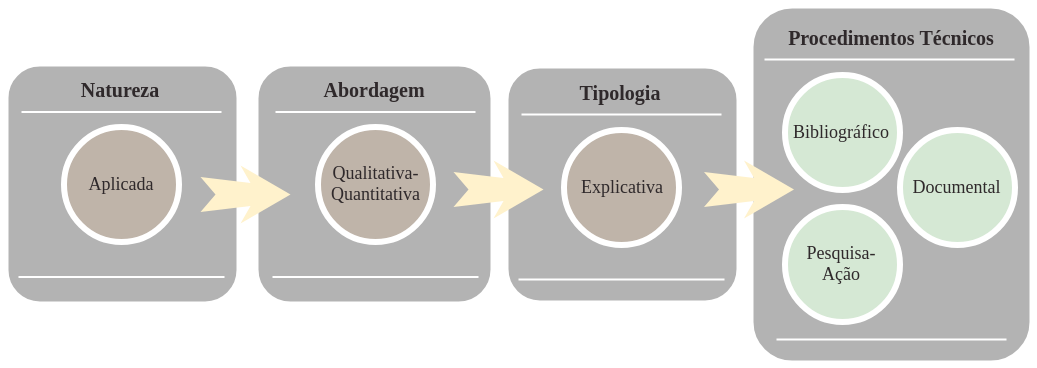
\includegraphics[width=14cm]{figuras/classificacaoMetodologica.png}
          \caption{Classificação Metodológica (Fonte: Elaborado pela Autora.)} 
          \label{fig:classificacaoMetodologica}
        
        \end{figure}
        
Dado que se busca criar um módulo em uma ferramenta, neste trabalho adotou-se a técnica de pesquisa-ação, que possibilita
ao pesquisador a construção de instrumentos em ciclos de iteração com a equipe, isso é, entre os pesquisadores e a organização alvo de estudos. Dessa forma, será possível a construção da ferramenta em ciclos de interação com o refinamento e validação do algoritmo de recomendação de \textit{tours} baseado em cada perfil de testador.

A Pesquisa-ação, proposta por~\cite{petersen2008systematic}, é empregada na especificação de um instrumento, com as etapas \textit{Diagnóstico, Planejamento da ação, Reflexão e Tomada de decisão}, cujo objetivo é a realização de ciclos de iteração para a especificação de um instrumento. E seguida da técnica Estudo de Caso, empregada na Construção do instrumento, cujo objetivo é desenvolver um sistema a partir da especificação definida de forma iterativa na fase anterior. Neste trabalho apresenta-se uma adaptação da proposta de ~\cite{petersen2008systematic}, na qual somente a pesquisa-ação será adotada.

Na Figura \ref{fig:etapasPesquisaAcaoAdotas} apresenta-se a fase Coleta de Dados e os procedimentos de pesquisa bibliográfica e de pesquisa-ação adotados neste trabalho.

        \begin{figure}[H]
          \centering
          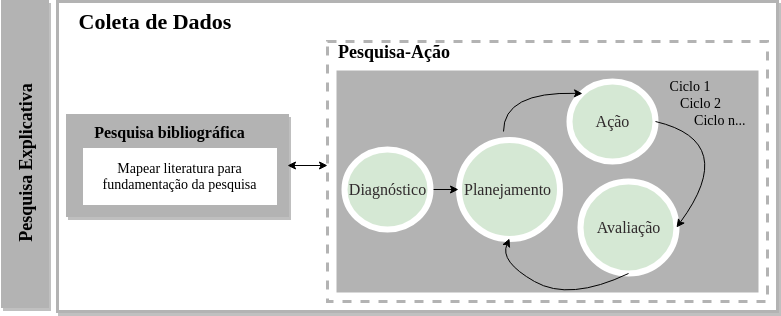
\includegraphics[width=12cm]{figuras/etapasPesquisaAcaoAdotadas.png}
          \caption{Etapas da Pesquisa-Ação adotadas. (Fonte: Adaptada de \cite{petersen2008systematic})} 
          \label{fig:etapasPesquisaAcaoAdotas}
        
        \end{figure}

O plano metodológico adotado neste trabalho compreendeu quatro fases básicas: \textit{planejamento da pesquisa}; \textit{coleta de dados}; \textit{análise dos dados}; e \textit{relato dos resultados}. O detalhamento deste planejamento metodológico encontra-se no Capítulo Materiais e Métodos.




    \section{Organização do Trabalho}

Este trabalho de conclusão de curso está organizado nos seguintes capítulos:

\begin{itemize}
    \item \textbf{Capítulo \ref{ch:introducao} - Introdução:} apresentou Contextualização, justificativa, problema de pesquisa, justificativa e objetivos;
    \item \textbf{Capítulo \ref{ch:referencial} - Referencial teórico:} descreve os conceitos que fundamentam o trabalho reunindo conhecimento necessário para que se compreenda a pesquisa realizada. O capítulo é subdividido nas seções \textit{Governo Digital}, \textit{Testes Exploratórios} e \textit{Sistema de Recomendação};
    % \item \textbf{Capítulo \ref{ch:suporte} - Suporte tecnológico:} apresenta as ferramentas que suportarão as atividades de desenvolvimento de software, gerenciamento, documentação, dentre outras.
     \item \textbf{Capítulo \ref{ch:metodologia} - Materiais e Métodos:} apresenta o plano metodológico adotado e caracteriza o objeto de estudo;
     \item \textbf{Capítulo \ref{ch:proposta} - Proposta:} Apresenta a proposta deste trabalho, desde a abordagem até a proposta de um módulo para a ferramenta de suporte ao processo de transformação digital do governo brasileiro.
     
    % \item \textbf{Capítulo \ref{ch:resultados} - Resultados parciais:} apresenta os resultados alcançados durante o TCC1.
    
    % \item \textbf{Capítulo \ref{ch:consideracoes} - Considerações finais:} relata o status do trabalho alcançado até a execução do TCC1 e os resultados esperados para o TCC2.
\end{itemize}

\chapter{Referencial Teórico}
\label{ch:referencial}

\section{Considerações Iniciais}
Neste capítulo apresentam-se a terminologia e conceitos básicos, visando facilitar o entendimento acerca dos principais temas desta pesquisa, este capítulo define os aspectos e elementos relacionados a sistema de
recomendação, perfil de testadores, testes exploratórios e governo digital.
%---------------- Governo Digital ---------------------%
\section{Governo Digital}

O advento da internet surgiu e reconfigurou o meio de comunicação para a população e, com o advento e evolução da tecnologia 
e expansão da internet surge a expressão \textit{Governo Digital}. Esta expressão se refere ao uso de tecnologias digitais como uma 
estratégia de modernização do Governo, que adota a tecnologia da informação e comunicação (TIC) para prover 
serviços e maximizar a eficiência de atividades governamentais~\cite{fang2002government}. 

O termo \textit{E-Governo} surgiu no final da década de 1990 e cresceu consideravelmente com 
diversas definições, como: governo mais eficiente, melhores serviços para o cidadão e um melhor processo 
democrático. Em sequência, nos últimos anos, o termo \textit{E-Governo} deu origem a várias conferências de cunho científico, aumentando seu 
conteúdo e posição no que se refere a outros campos de pesquisa e disciplinas~\cite{gronlund2005introducing}.

A OECD (\textit{Organisation for Economic Co-operation and Development}) usa a expressão \textit {Governo Eletrônico} como o uso de 
Tecnologias de Informação e Comunicação pelo governo, que se refere a uma ferramenta que busca melhorar as atividades do governo, 
especialmente, com do uso da Internet. A expressão \textit{Governo Digital}, por outro lado, refere-se ao uso de tecnologias 
digitais que buscam adicionar valor público como parte complementar às estratégias de modernização de um governo.

A integração de novas tecnologias no cotidiano faz com que as expectativas dos cidadãos sobre suas relações com os governos mudem~\cite{oecd}, visto que as opiniões e necessidades podem passar a ser consideradas de forma mais eficaz, trazendo a possibilidade 
de realizar processos governamentais com maior facilitade e agilidade. Esta consolidação das expectativas criadas sobre o governo exige que novas abordagens de governança pública possam trazer a digitização de serviços,
considerando-se que, através da desburocratização de alguns serviços e processos, os cidadãos e empresas podem ser integrados ao meio digital.

Embora as medidas de modernização do setor público tenham começado a ser adotadas na década de 70, a dedicação, de fato, apareceu apenas em decorrência da crise fiscal dos anos 80, quando a intervenção estatal se popularizou como reforma da gestão pública que, aliada às TICs, disponibilizou serviços públicos eletrônicos à população no início da década de 2000~\cite{przeybilovicz2015desenvolvimento}.

O conceito de E-Governo envolve um aglomerado de responsabilidades que impactam em todos os níveis sociais. De acordo com \cite{fang2002government}, o conceito de E-governo possui três grandes focos: 

\begin{itemize}
    \item \textbf{E-Government}: Referente as atividades internas do governo, sejam administrativas, organizacionais ou de comunicação. 
    \item \textbf{E-Commerce}: Responsável pela interface entre o governo e o mercado.
    \item \textbf{E-Citizens}: Suporte para interface entre governo e cidadão, possibilitando a disponibilização de serviços de maneira prática e eficiente.
\end{itemize}

A Figura \ref{img:triangulo} apresenta o modelo de relacionamento entre E-Government, E-Commerce e E-Citizens.

\begin{figure}[!htb]
\centering
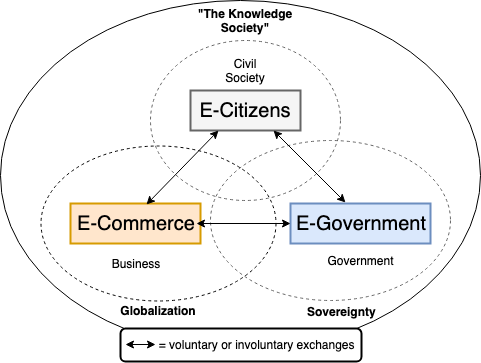
\includegraphics[width=0.7\textwidth]{figuras/relacao_triangular_e-gov.png}
\caption{Modelo de Relacionamento Triangular: Governo Eletrônico, Negócios e Cidadãos. Adaptado de \cite{fang2002government}.}
\label{img:triangulo}
\end{figure}

Neste sentido, o conceito de Governo Digital envolve diversos âmbitos, evidenciando a grandeza e importância de um processo de transformação digital no governo.


\section{Transformação Digital no Brasil}

No Brasil, em 2016, somente 54\% dos domicílios brasileiros possuíam acesso à internet, o que representa 6,7 milhões de residências e um total de 107,9 milhões de usuários de Internet~\cite{CGI}. Neste mesmo ano, ocorreu o lançamento da \textit{Estratégia de Governança Digital da Administração Pública Federal} (EGD), com o objetivo de definir estratégias, metas e indicadores da Política de Governança Digital. A partir da EGD, a prestação de serviços
públicos poderia ser simplificada e agilizada proporcionando uma melhoria no ambiente de negócios e eficiência da gestão pública.

Ainda em 2016, o Decreto número 8.638 foi publicado pela Casa Civil da Presidência da República \cite{BRASIL2016c}, instituindo a Política de Governança Digital, no âmbito dos órgãos e das entidades da administração pública federal direta, autárquica e fundacional. 

% No Decreto número 8.638 \cite{BRASIL2016c}, existem dois artigos a serem destacados por seus princípios e objetivos, estes estão 
% listados na tabela a seguir:

Para estimular a transformação dos serviços públicos em serviços digitais, de modo que estes ocorram por meio eletrônico, o governo
brasileiro publicou decretos relevantes entre 2014 e 2016, como citado ao longo desta seção. Os decretos definiram a Política de Governança
Digital e a Plataforma de Cidadania Digital, no âmbito da Administração Pública Federal (APF), ambos de responsabilidade do então 
Ministério do Planejamento, Desenvolvimento e Gestão (MP) \cite{BRASIL, BRASIL2016}. 

A Plataforma de Cidadania Digital configura um conjunto de metodologias e soluções que buscam ampliar e simplificar o acesso dos cidadãos aos serviços digitais e, também, para apoiar os órgãos públicos na aceleração da transformação digital de serviços.  

Simultaneamente às ações da Plataforma de Cidadania Digital, o Departamento lançou um canal para oferecer informações no
formato de um portal de serviços do Governo Federal\footnote{https://www.servicos.gov.br/}. A iniciativa surgiu para permitir o arquivamento de solicitações eletrônicas e monitorar os serviços públicos pelos usuários. Juntamente com o portal, foi lançado um programa de automação de serviços públicos, para a tentativa de orientar e apoiar órgãos públicos a identificar, priorizar, digitalizar e implementar serviços 
com mais qualidade e transparência para os cidadãos.

Um dos objetivos do governo brasileiro com a transformação digital é ampliar os serviços públicos nos canais digitais. 
Atualmente, o governo oferece aproximadamente 1.700 serviços, mas apenas 41\% são totalmente digitais. Vale ressaltar que o processo de transformação brasileiro envolve os três principais focos apresentados na Figura \ref{img:triangulo}: \textit{E-Government}, \textit{E-Commerce} e \textit{E-Citizens}.

Tendo em vista os decretos publicados, o Departamento \textbf{INOVA} do antigo MP, se responsabilizou pela construção de um programa de Governo Digital, denominado \textit{Kit de Transformação}. O objetivo é, de modo geral, transformar os serviços públicos a partir da utilização de um kit, ao invés da adoção de uma metodologia, por exemplo, objetivando facilitar a adoção e orientação aos diversos órgãos da APF.

O \textit{Kit de Transformação} é composto por seis estágios de aplicações independentes, como demonstrado na Figura \ref{fig:EtapasTransform}.

        \begin{figure}[h]
          \centering
          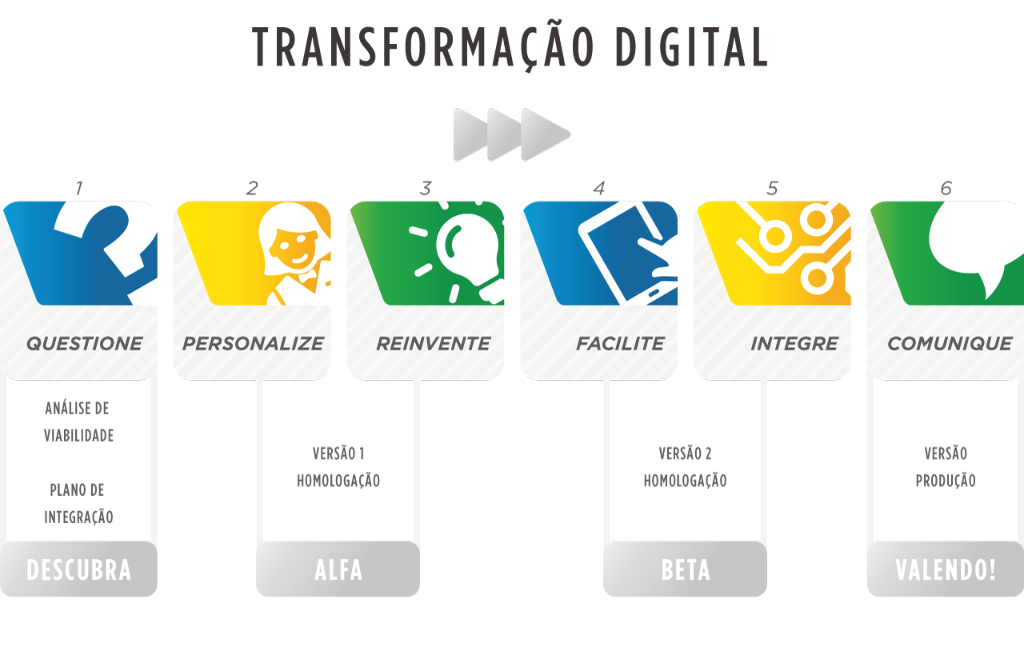
\includegraphics[width=15cm]{figuras/secao-referencial/EtapasTransform.png}
          \caption{Fases do Kit de Transformação (Fonte: \cite{BRASIL2017})} 
          \label{fig:EtapasTransform}
        \end{figure}
        
        
A seguir é apresentado cada um dos estágios destacados na Figura \ref{fig:EtapasTransform}:

\begin{itemize}
\item \textbf{Questione}

Esta fase foi delineada para que o órgão fosse capaz de identificar e priorizar seus principais serviços, além de realizar um diagnóstico que anteceda a transformação, de modo que uma avaliação posterior resulte nos anseios dos usuários. A metodologia desta fase busca, especificamente, a identificação de serviços, avaliação da maturidade da gestão em serviços, levantamento de custos dos usuários do serviço, priorização da transformação de serviços e, por fim, o diagnóstico e avaliação dos serviços.

\item \textbf{Personalize}
Nesta fase é utilizada a visão do usuário como um propósito para que se atinja serviços personalizados, sendo assim, o ministério busca identificar as necessidades do usuário a fundo para que se mapeie as impressões mais relevantes sobre os problemas levantados. A partir do levantamento das necessidades mais relevantes dos usuários, pode-se conseguir dados sobre o acesso, uso, satisfação e expectativas sobre o serviço prestado, além da análise de qualidade do serviço em questão.


\item \textbf{Reinvente}


É importante que a transformação seja analisada, sintetizada, prototipada e testada, por isso, esta fase realiza a definição do Serviço Mínimo Viável (SMV). Partindo desta definição torna-se possível escolher alternativas de solução e possibilidades de se encontrar um melhor trajeto para a iniciação da transformação de serviços. É fundamental nesta fase que se crie novas soluções para aprimorar e estimular o processo de transformação deste contexto.


\item \textbf{Facilite}


A ideia da fase Facilite é oferecer um guia de simplificação de serviços ao participante. É a partir desta fase que se configuram ferramenta de agendamentos, ferramenta de automação de serviços públicos, solução de peticionamento eletrônico do SEI (Sistema Eletrônico de Informações) e solução de atendimento virtual.



\item \textbf{Integre}


Ao solicitar um serviço, o cidadão precisa disponibilizar tempo e custo logístico para obter a apresentar determinados documentos que são requeridos. Sendo assim, o objetivo desta fase é integrar suas bases de dados às plataformas criadas de modo que, o acesso dos cidadãos aos serviços sejam simplificados, com dados unificados. Com a integração das informações dos usuários pode-se eliminar a necessidade de que se apresente dados já cadastrados pelo cidadão, ou seja, as bases do governo que já capturaram determinadas informações, passam a reutilizá-las em diversas situações, minimizando o esforço por parte do cidadão.


\item \textbf{Comunique}


Para que se planeje e comunique aos cidadãos as mudanças realizadas, é necessário que o órgão defina e avalie ações de comunicação. Para tanto, a fase Comunique necessita da transformação do serviço pronta para ser implantada, com seus respectivos canais de atendimento para a transformação do serviços. 

\end{itemize}

Por meio das ferramentas da fase \textit{Questione}, o órgão parceiro poderá avaliar em que medida as ferramentas das demais fases serão úteis para melhorar seus serviços. Com isso, o órgão parceiro terá parâmetros para decidir se utilizará o conjunto completo do Programa ou se adotará uma ``\textit{estratégia de prateleira}'', selecionando aleatoriamente as ferramentas de que necessita.

Para a fase Facilite, o Ministério contratou, por meio de licitações, uma empresa que fornece uma ferramenta de digitalização de serviços baseada no conceito de \textit{meta-design}~\cite{fogli2012meta}. Após a digitalização, os serviços devem ser validados e entregues a população. 

O ITRAC, da UnB, em seu projeto de parceria com o então Ministério do Planejamento, contribuiu para o programa de automatização no quesito da garantia da qualidade dos serviços transformados.



%---------------- Testes Exploratórios-----------------%
\section{Processo de Testes definidos pelo ITRAC}

A busca pela simplificação  e transformação de serviços utilizando das soluções tecnológicas que a empresa terceiriza proporciona está relacionada à problemática de se testar sem requisitos. A transformação digital que se ocorre não garante requisitos estáveis ou, até mesmo, a existência de requisitos e isto pode resultar em um problema definido como Problema do Oráculo~\cite{barr2015oracle}. 

O cenário de requisitos instáveis dificulta a identificação do comportamento atual do serviço digitalizado ao ser comparado com o comportamento esperado, ou ao ser analisado como um comportamento errado.  Além disso, devido a forma de contratação definida, o código-fonte dos serviços transformados não são disponibilizados, o que dificulta mais ainda o processo de testes e a extração de informações por parte da equipe de testes.

Levando todo o contexto da transformação dos serviços em consideração, foi desenvolvido um processo de validação sistematizado, com o intuito de garantira qualidade da digitalização dos serviços. As etapas de criação e execução de casos de teste de cada serviço podem ser realizadas usando diversos padrões de teste, desde estratégias de teste manual até testes automatizados. 

O processo de validação dos serviços digitizados  definido pelo ITRAC está de acordo com o apresentado na Figura \ref{img:process_test}.
 
 \begin{figure}[H]
 \centering
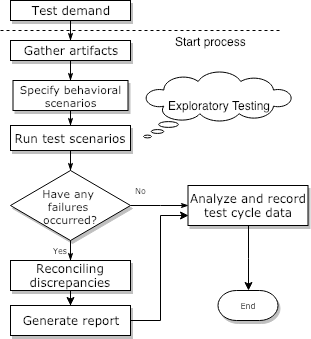
\includegraphics[width=0.7\textwidth]{figuras/Processo_artigo_menor.png}
\caption{Processo de Validação de Serviços definido pelo ITRAC adaptado de~\cite{elcock2006testing}.}
\label{img:process_test}
\end{figure}

Visto que o código-fonte não é acessível pelo ITRAC e o conjunto de requisitos não é bem definido, o processo proposto pelo ITRAC se baseia na estratégia proposta por \cite{elcock2006testing} e no conceito de Teste Exploratório (ET), sugerido por \cite{whittaker2009exploratory}, usando a metáfora do turista como uma estratégia para guiar, através das chamadas ``tours'', a descoberta de requisitos e regras de negócios, além de sistematizar a criação e execução dos casos de teste. O conceito de Testes Exploratórios utilizado como base para definição do processo de teste será apresentado, de maneira detalhada, na Seção \ref{sec:testes_exploratorios}.


A partir da padronização do processo de teste definida pelo ITRAC, foi possível iniciar o desenvolvimento de uma ferramenta de apoio ao processo de teste dos serviços digitizados. A ferramenta, chamada \textit{Digital Transformation Environment Support Tool}, ou DTEST é apresentada a seguir.

\subsection[DTEST]{Ferramenta DTEST -- Digital Transformation Environment Support Tool}
\label{sec:dtest}

A partir da análise das características envolvidas no processo de Transformação Digital brasileiro, foi definida uma ferramenta de apoio ao processo de transformação, representada pela Figura \ref{img:architecture}, a qual tem como objetivo maximizar a eficiência do processo de transformação digital no governo brasileiro.

\begin{figure}[!htb]
\centering
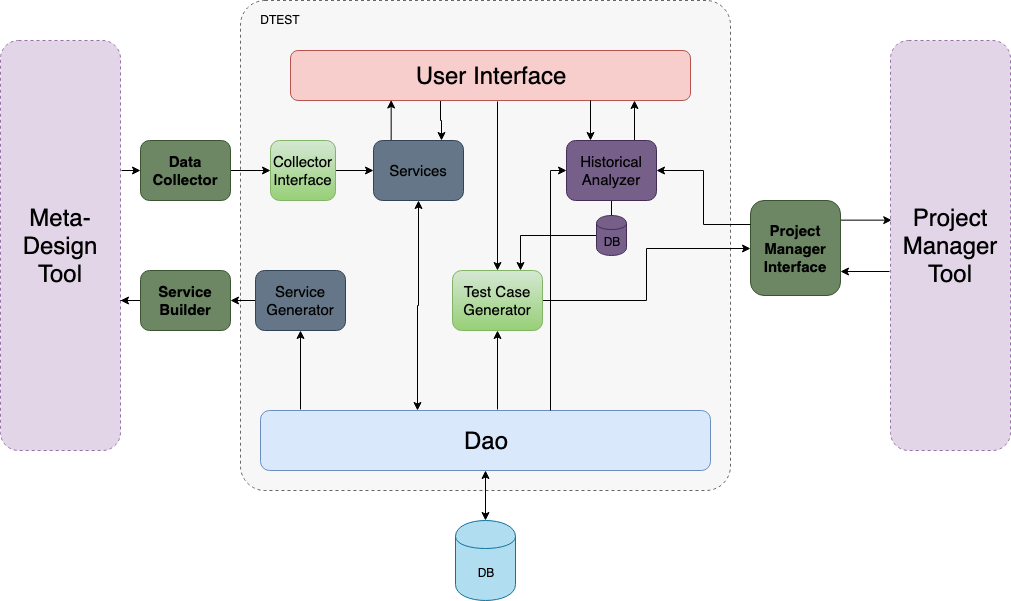
\includegraphics[width=1\textwidth]{figuras/arquitetura_sem_tester.png}
\caption{Arquitetura DTEST (Fonte: Elaborado pela Autora.)}
\label{img:architecture}
\end{figure}

O principal objetivo da ferramenta é facilitar a realização das atividades relacionadas ao processo de Transformação Digital no governo brasileiro. Dessa forma, a \itractool se baseia na utilização de ferramentas geradoras de produtos de software com base em estratégias de meta-design e EUD. Considera-se, também, que ferramentas de gerenciamento de projetos são utilizadas como forma de gerenciamento e acompanhamento das atividades do processo de transformação. Dessa forma, de acordo com o apresentado na Figura \ref{img:architecture}, a \itractool se encontra entre a ferramenta de meta-design e a ferramenta de gerenciamento de projeto utilizada pela equipe de Transformação Digital. 

O componente central da arquitetura apresentada na Figura \ref{img:architecture} agrupa os módulos da \itractool. Os módulos destacados na cor verde escuro, ``Data Collector" e ``Project Manager Interface", são módulos a parte e que devem ser definidos de acordo com o contexto em que a \itractool será utilizada. Esta estrutura de componentes objetiva a aplicabilidade da ferramenta proposta em diversos contextos, garantindo, ainda, a generalidade e replicabilidade do trabalho apresentado.

A seguir são apresentados os principais módulos envolvidos no ambiente da ferramenta \itractool.

\begin{itemize}
    \item O módulo \textit{Data Collector} é responsável pela extração de informações na ferramenta de meta-design. Esta extração pode ser realizada como a equipe desejar. No nosso contexto, a extração precisou ser feita via \textit{web crawler}, mas poderia ser feita via API ou acesso ao banco de dados, por exemplo. A partir da obtenção dos dados, estes são mapeados em entidades do tipo \textit{Service} e registrados no banco de dados para consulta dos próximos módulos. 
    
    \item O módulo \textit{Collector Interface} é responsável por definir as regras de interface para integração do módulo \textit{Data Collector}.
    
    \item O módulo \textit{Services} é responsável pelo gerenciamento do serviços extraídos. Constrói e distribui as relações entre cada entidade dos serviços, estas relações podem ser denominadas e enxergadas no código como \textit{Stages} e \textit{Fields}. Este também é responsável por registrar todas as informações de serviços no banco de dados para consulta de outros módulos. 
    
    % \del{Acho que nesse ponto, ainda não foi dito o que são Stages e Fields. Acredito que, se for o caso, poderia se descrever, quando se fala da ferramenta de Meta-Design, no que consiste um serviço e como o meta-modelo faz esse mapeamento para esclarecer isso.}
    
    \item O módulo \textit{Test Case Generator} é o módulo responsável pela geração automática de casos de teste para validar determinado serviço digitizado.
    
    \item O módulo \textit{Tester Manager} é responsável pelo gerenciamento de atividades de teste. Entre os objetivos deste módulo está a Atribuição de \textit{tours} nesse caso específico para testadores com base em características de ambos testadores e tours.
    
    \item O módulo \textit{Historical Analyzer} é responsável pela análise dos dados históricos para melhoria contínua do processo de transformação. 
    
    \item O módulo \textit{Project Manager Interface} é responsável pela formatação dos dados resultantes para registro na ferramenta de gerenciamento de projeto utilizada pela equipe. Este também é responsável pela extração de informações de gerenciador de projeto para gerar informação para o módulo \textit{Historical Analyzer}.
\end{itemize}

De maneira mais detalhada, as principais funcionalidades presentes na ferramenta são apresentadas a seguir.

\subsubsection{Suporte à Validação}
\label{sec:teste}

A partir da experiência obtida com a garantia da qualidade dos serviços advindos do contexto brasileiro de Transformação Digital, foi possível definir estratégias automatizadas para maximizar a eficiência da atividade de validação. O processo de validação dos serviços se baseia na utilização do conceito de Testes Exploratórios de tal forma que possibilitou a padronização e sistematização dos casos de teste por meio dos tours. A partir desta padronização foi possível criar uma estrutura para geração automatizada de casos de teste com base nas características do SUT.

Como o contexto brasileiro de TD se baseia em estratégias de meta-design e EUD para desenvolvimento do serviços, a extração das características de cada serviço é uma atividade passível de automação. No nosso contexto, foi desenvolvido um script em Python para extração de informação de cada serviço a partir da execução de um \textbf{web crawler} na ferramenta de meta-design utilizada. A partir da obtenção de todas as informações necessárias, é possível fazer a geração automatizada de casos de teste.

A estratégia de extração de informações dos serviços digitizados segue o padrão utilizado pela ferramenta de meta-design adotada pelo governo brasileiro. Deste modo, observa-se que um \textbf{Service} possui uma ou mais \textbf{Stages} e muitos \textbf{Fields}. Entretanto, vale destacar que cada \textbf{Field} está associado a todas as \textbf{Stages} do serviço, entretanto com configurações diferentes (somente leitura, obrigatório, opcional e etc). A partir desta estrutura de relacionamento, o Algorithm \ref{test_case_generation} apresenta a lógica utilizada para geração dos casos de teste com base nas características do SUT.

    \begin{algorithm}[!htb]

	\KwIn{Service service}
	\KwResult{List tests}

	\SetKwProg{Fn}{Function}{}{}
	\Fn{generate\_test\_cases(service)}{
	   tests = []\;
	   
	   \For{service.stages as stage}{
	        tests.append(test\_cancel\_stage(stage))\;
	        
	        \For{stage.stage\_fields as stage\_field}{
	            type = verify\_type(stage\_field)\;
	            tests.append(create\_test(type, stage\_field))\;
	        
	        }
	   }
        % \If{not f\_base}{
        %     feature.save()\;
        % }
		\Return{tests}\;
	}
\caption{Test Case Generation.}
\label{test_case_generation}
\end{algorithm}

A linha 3 do Algoritmo~\ref{test_case_generation} extrai todas as \textbf{Stages} de um serviço e itera sobre elas. Para cada \textbf{Stage}, um caso de teste baseado na Tour Período Chuvoso (Metáfora do Turista \cite{whittaker2009exploratory}) é gerado, validando o funcionamento correto da opção de cancelar a \textbf{Stage} atual.

Outros casos de teste genéricos para qualquer \textbf{Stage} devem ser incluídos após a linha 3 e antes da linha 5. Após a linha 5 do Algoritmo~\ref{test_case_generation}, cada relação Stage-Field é analisada para geração de casos de teste específicos com base na configuração de cada \textbf{Field} em cada \textbf{Stage}. Com esta estrutura, basta identificar casos de teste adequados a determinadas características do serviço e incluí-lo como uma nova verificação dentro do método \textit{create\_test()}. A Tabela~\ref{tab:test_types} apresenta os tipos de teste já cobertos pela \textbf{ITRACtool}.


\begin{table}[htb!]
\centering
\caption{Current types of auto-generated test cases.}
\label{tab:test_types}
\begin{tabular}{|c|c|c|}
\hline
\textbf{Field Type}                                                                   & \textbf{Test Case}                                                       & \textbf{Description}                                                                                                                                            \\ \hline
\textit{\begin{tabular}[c]{@{}c@{}}Required \\ Field\end{tabular}}                    & \begin{tabular}[c]{@{}c@{}}Test required \\ fields\end{tabular}          & \begin{tabular}[c]{@{}c@{}}Validate the exception \\ obtained with the \\ submission of the form \\ without the inclusion of \\ the required field\end{tabular} \\ \hline
\multirow{2}{*}{\textit{\begin{tabular}[c]{@{}c@{}}Normal \\ (Visible)\end{tabular}}} & \begin{tabular}[c]{@{}c@{}}Test help \\ text\end{tabular}                & \begin{tabular}[c]{@{}c@{}}Validate the help \\ text message in\\ each visible Field.\end{tabular}                                                              \\ \cline{2-3} 
                                                                                      & \begin{tabular}[c]{@{}c@{}}Test field \\ label\end{tabular}              & \begin{tabular}[c]{@{}c@{}}Verify field label \\ consistency\end{tabular}                                                                                       \\ \hline
\textit{Email}                                                                        & \begin{tabular}[c]{@{}c@{}}Test email \\ field\end{tabular}              & Validate invalid email                                                                                                                                          \\ \hline
\multirow{2}{*}{\textit{Data}}                                                        & \begin{tabular}[c]{@{}c@{}}Test Date \\ field\end{tabular}               & Validate invalid Date                                                                                                                                           \\ \cline{2-3} 
                                                                                      & \begin{tabular}[c]{@{}c@{}}Test Date \\ modal\end{tabular}               & \begin{tabular}[c]{@{}c@{}}Validate the date \\ modal format\end{tabular}                                                                                       \\ \hline
\multirow{4}{*}{\textit{Template}}                                                    & \begin{tabular}[c]{@{}c@{}}Test \\ template\end{tabular}                 & \begin{tabular}[c]{@{}c@{}}Submit an invalid format \\ or size\end{tabular}                                                                                     \\ \cline{2-3} 
                                                                                      & \begin{tabular}[c]{@{}c@{}}Test \\ template\\ specification\end{tabular} & \begin{tabular}[c]{@{}c@{}}Validate the\\ required file specification\end{tabular}                                                                              \\ \cline{2-3} 
                                                                                      & \begin{tabular}[c]{@{}c@{}}Test template \\ size\end{tabular}            & \begin{tabular}[c]{@{}c@{}}Validate the max \\ size accepted\end{tabular}                                                                                       \\ \cline{2-3} 
                                                                                      & \begin{tabular}[c]{@{}c@{}}Test template\\ modal\end{tabular}            & \begin{tabular}[c]{@{}c@{}}Validate the template \\ modal format\end{tabular}                                                                                   \\ \hline
\textit{Phone}                                                                        & \begin{tabular}[c]{@{}c@{}}Test mask\\ phone\end{tabular}                & \begin{tabular}[c]{@{}c@{}}Verify valid and invalid \\ masks for phones\end{tabular}                                                                          \\ \hline
\end{tabular}
\end{table}

Desse modo, o serviço analisado passa por uma inspeção que busca características específicas do serviço para geração de casos de teste. Como resultado da atividade de geração de casos de teste, encontra-se uma lista de casos de teste formatados de tal forma que seja possível a inclusão destes em uma ferramenta de gerenciamento de projetos, para registro e acompanhamento do caso de teste.

\subsubsection{Generation Support}
\label{sec:geracao}

% Dado que a transformação do serviços é feita a partir da utilização de ferramentas de meta-design, é possível identificar pontos de automação que possibilite maximizar a eficiência desta atividade. 
De acordo com a experiência obtida ao longo do primeiro ano de transformação digital, algumas atividades mecânicas puderam ser destacadas, como a construção do serviço, criando as \textbf{Stages} e \textbf{Fields} associados, assim como a configuração de cada \textbf{Field} em suas respectivas \textbf{Stages}. Esta atividade mecânica e repetitiva foi automatizada a partir da implementação dos módulos \textit{``Service Generator"} e \textit{``Service Builder"}, apresentados na Figura \ref{img:architecture}.

Este objetivo é alcançado a partir da definição das características do serviço desejado utilizando a \itractool, exportando essas características para a ferramenta de meta-design. A estratégia adotada para exportar o serviço foi a utilização de um \textbf{web crawler} escrito em Python, responsável por navegar pela ferramenta de meta-design e criar as \textbf{Stages} necessárias, seus respectivos \textbf{Fields} e, consequentemente, suas configurações de visualização e comportamento.

Vale ressaltar que a estratégia de geração de serviços na ferramenta de meta-design deve ser definida de acordo com as características envolvidas. Em alguns casos, algumas adaptações devem ser realizadas, de acordo com o funcionamento da ferramenta de meta-design utilizada pela equipe de transformação.

% Os conceitos utilizados para a definição da estratégia dos testes serão descritos nas seções x, y e z.

De acordo com o apresentado nesta seção, a ferramenta \itractool trabalha com diversas informações úteis para o contexto analisado nesta pesquisa. Dessa forma, a proposta de abordagem apresentada neste trabalho deverá se relacionar com a ferramenta \itractool.

\section{Testes Exploratórios}
\label{sec:testes_exploratorios}

 No contexto do ciclo de vida do desenvolvimento de software, a atividade de teste é de suma importância, visto a sua capacidade de avaliar e melhorar a qualidade do software \cite{bertolino2007software}. Existem diversas técnicas para cumprir o teste sistemático de software, seja teste caixa preta, caixa branca e caixa cinza. Dessa forma, testadores utilizam diferentes técnicas para encontrar e solucionar defeitos com o menor esforço possível \cite{maldonado2004introduccao}. 

A realização de teste por parte de testadores humanos é relevante no desenvolvimento de software do mundo real por facilitar a identificação de novos BUGs, especialmente no contexto de sistemas interativos. Testadores humanos têm vantagens sobre máquinas, visto a capacidade de conhecimento, aprendizado e adaptação a novas situações, que facilita o processo de reconhecimento eficiente de dos problemas~\cite{itkonen2015test}. 

O ato de explorar pode ser consolidado quando não se sabe ao certo qual caminho traçar para se chegar a determinado ponto, este ato é análogo ao teste de software, porque busca descobrir informações sobre a qualidade do sistema a ser testado~\cite{itkonen2015test}.

O Teste Exploratório (TE) é uma abordagem de teste manual que emerge com um potencial de adaptação para os testes a partir de um processo de aprendizagem, utilizando de uma visão mais humana e relacionada à experiência dos envolvidos. Esta abordagem de teste foi mostrada na indústria de software com seus primeiros materiais produzidos aparecendo em blogs da internet~\cite{kaner2000testing} e, em 2009, aparecendo em livros e artigos. 

O termo também aparece em \textbf{SWEBOK}~\cite{bourque2014guide}, onde é definido simultaneamente como aprendizagem, o projeto de teste 
e a execução do teste, ou seja, os testes são definidos antecipadamente em um plano de teste estabelecido, mas 
são dinamicamente projetados, executados e modificados.

Por meio do teste exploratório, é possível que o testador não dependa de um conjunto de casos de teste pré-projetados, visto que, dentro dessa abordagem de teste existem etapas de \textit{design} e execução de testes, nas quais os testadores estão constantemente aprendendo e 
adaptando suas atividades. De maneira prática, o testador aprende iterativamente sobre o produto e suas falhas, projeta e executa os testes de forma dinâmica~\cite{whittaker2009exploratory}, mas sistemática. Os tours permitem aos testadores se recordarem dos objetivos do teste e, desse modo, mesmo que os testes sejam feitos de forma manual e exploratória, a forma de exploração fica sistematizada quando testador procura atingir o objetivo do tour.

A Tabela~\ref{tab:comparativo} apresenta uma adaptação da comparação realizada por \cite{itkonen2015test}, na qual se observa a repetibilidade mecânica, orientada por documentos na execução do teste. A abordagem de testes exploratórios destaca o conhecimento, a aprendizagem e a descoberta de novas informações que proporcionam um conhecimento mais aprofundado do software. 

O teste exploratório apresenta objetivos semelhantes aos testes automatizados, entretanto, o TE não utiliza descrições formais ou metodologias detalhadas, além da não necessidade de acesso ao código-fonte, o que faz com que sua abordagem seja mais adequada ao contexto da transformação digital de serviços, parte deste trabalho. 

% Please add the following required packages to your document preamble:
% \usepackage{graphicx}
% \usepackage[table,xcdraw]{xcolor}
% If you use beamer only pass "xcolor=table" option, i.e. \documentclass[xcolor=table]{beamer}
\begin{table}[!htb]
\caption{Comparativo entre teste automatizado, teste manual (\textit{ad-hoc}) e teste exploratório. Adaptado de \cite{itkonen2015test}.}
\label{tab:comparativo}
\resizebox{\textwidth}{!}{%
\begin{tabular}{|l|l|l|l|}
\hline
\rowcolor[HTML]{333333} 
{\color[HTML]{FFFFFF} } & {\color[HTML]{FFFFFF} \textbf{Automatizado}} & {\color[HTML]{FFFFFF} \textbf{Manual (ad-hoc)}} & {\color[HTML]{FFFFFF} \textbf{Teste Exploratório}} \\ \hline
\rowcolor[HTML]{FFFFFF} 
\textbf{\begin{tabular}[c]{@{}l@{}}Filosofia \\ de Teste\end{tabular}} & Automatizado e repetitivo para oferecer feedback & \begin{tabular}[c]{@{}l@{}}Mecânico, repetitivo \\ e descrito em instruções explícitas.\end{tabular} & \begin{tabular}[c]{@{}l@{}}Conhecimento intensivo,\\ atividade criativa que requer habilidades.\end{tabular} \\
\rowcolor[HTML]{EFEFEF} 
\textbf{\begin{tabular}[c]{@{}l@{}}Design \\ de Teste\end{tabular}} & \begin{tabular}[c]{@{}l@{}}Design desafiador e caro, \\ mas de execução rápida e barata.\end{tabular} & Design separado e sequencial. & \begin{tabular}[c]{@{}l@{}}Design e execução paralelos; \\ Requer aprendizagem exploratória \\ do teste.\end{tabular} \\
\rowcolor[HTML]{FFFFFF} 
\textbf{Documentação} & \begin{tabular}[c]{@{}l@{}}Certos tipos de testes podem ser \\ roteirizados e automatizados.\end{tabular} & \begin{tabular}[c]{@{}l@{}}O teste pode ser distribuído para\\ diversos tipos de pessoas \\ com base nos testes documentados.\end{tabular} & \begin{tabular}[c]{@{}l@{}}Requer conhecimento e habilidades\\ difíceis de transferir com\\ a documentação.\end{tabular} \\
\rowcolor[HTML]{EFEFEF} 
\textbf{\begin{tabular}[c]{@{}l@{}}Conhecimentos \\ Necessários\end{tabular}} & \begin{tabular}[c]{@{}l@{}}Certos tipos de bugs podem ser \\ efetivamente detectados\\ automaticamente.\end{tabular} & \begin{tabular}[c]{@{}l@{}}Previsão de erros;\\ Resultados esperados documentados \\ para simples comparação de \\ tempo de execução.\end{tabular} & \begin{tabular}[c]{@{}l@{}}Os bugs são imprevisíveis e requerem\\ conhecimento do sistema e do domínio\\ da aplicação para detecção.\end{tabular} \\
\rowcolor[HTML]{FFFFFF} 
\textbf{Repetibilidade} & \begin{tabular}[c]{@{}l@{}}Repetibilidade e execução de testes em ciclos \\ muito curtos, mecessita de feedback rápido \\ sobre a regressão durante o desenvolvimento.\end{tabular} & \begin{tabular}[c]{@{}l@{}}Repetibilidade essencial; \\ Descrições exatas de casos de teste reduzem \\ a variação individual nos testes.\end{tabular} & \begin{tabular}[c]{@{}l@{}}Repetir os mesmos testes \\ não revela novos bugs nem\\ novas informações sobre a qualidade,\\ oferecendo pouco valor agregado.\end{tabular} \\
\rowcolor[HTML]{EFEFEF} 
\multicolumn{1}{|c|}{\cellcolor[HTML]{EFEFEF}\textbf{Automatização}} & \begin{tabular}[c]{@{}l@{}}Os testes devem ser \\ automatizados o máximo possível.\end{tabular} & \begin{tabular}[c]{@{}l@{}}Testadores humanos podem ser usados\\ para objetivos semelhantes aos da automação.\end{tabular} & \begin{tabular}[c]{@{}l@{}}A automação deve ser usada \\ para aprimorar os testes \\ e liberar recursos humanos para outros \\ tipos de atividades de teste.\end{tabular} \\ \hline
\end{tabular}%
}
\end{table}

\subsection{Metáfora do Turista}

Para sistematizar o processo de TE, \cite{whittaker2009exploratory} propôs a Metáfora do Turista, a qual consiste na analogia entre um turista em uma cidade e o teste de software. Segundo \cite{whittaker2009exploratory}, o turismo é uma mescla entre estrutura e liberdade, assim como o teste exploratório. Dessa forma, ele definiu a metáfora do turista com o objetivo de auxiliar na construção dos testes.

Na analogia apresentada, as funcionalidades dos softwares são separadas em distritos, que significam a delimitação de um espaço que se decide explorar, o que, na prática, representa as diferentes áreas do software. Além disso,  cada distrito possui um conjunto de ``tours'', que representam as diferentes maneiras de percorrer as diferentes características e funcionalidades do software. A seguir, são destacados alguns dos distritos mais utilizados pela equipe e suas respectivas ``tours'':

\subsubsection{Distrito Hoteleiro}

 É geralmente onde o turista descansa depois de um dia cheio de passeios e fica longe da agitação da viagem. Em um software, esse distrito representa os recursos secundários do aplicativo, normalmente ignorados ou deixados de lado. Em relação a este distrito, as ``tours'' utilizadas neste trabalho de pesquisa foram:

\begin{itemize}
    \item \textbf{Tour em Período Chuvoso}: Um turista pode se encontrar em um dia chuvoso e sentir vontade de tornar o passeio mais curto ou até mesmo cancelá-lo. No software, a recomendação é que o testador, ao fazer as ``tours'', use as opções que interrompem o processo do sistema. Os recursos que exigem processamento de intervalo de tempo e fornecem uma opção de cancelamento durante o preenchimento de algumas informações devem ser iniciados e cancelados, com o objetivo de verificar se as opções de cancelamento funcionam adequadamente em qualquer contexto.
    
    \item \textbf{Tour com Desinteressados}: Ao passear em uma cidade turística, alguns turistas podem parecer preguiçosos e desinteressados, não curtindo o passeio e o guia turístico pode ter que se esforçar mais para entretê-los. No contexto do software, os testadores desinteressados podem ser muito eficazes. A ``tour'' consiste em fazer o sistema funcionar fornecendo o mínimo de dados possível, forçando-o a se alinhar com valores padrão e entradas vazias.
\end{itemize}

\subsubsection{Distrito Decadente} 

Local onde costumam ocorrer alarmes constantemente. No software, essas ``tours'' têm como objetivo fornecer ações que podem causar falhas no software. As ``tours'' utilizadas nesta pesquisa foram:

\begin {itemize}
    \item \textbf {Tour Sabotador}: Todas as oportunidades para sabotar o aplicativo devem ser usadas. Nesta ``tour'', o testador deve forçar o software a iniciar alguma operação, identificar os recursos necessários para terminá-lo e remover esses recursos. Deve-se, por exemplo, solicitar que o aplicativo leia algo no disco, mas sabotar a tentativa de leitura para causar confusão, levando o sistema a falhar.
    \item \textbf {Tour Antissocial}: Em um passeio pela cidade, o turista anti-social é aquele que mostra claramente a insatisfação com o passeio e faz questão de encontrar algo para se opor a tudo o que é visto ou falado durante o passeio. Para testadores, é indispensável ter esse aspecto anti-social, com o objetivo de procurar por todos os tipos de possíveis falhas no software. A ``tour'' anti-social consiste em inserir entradas que nunca devem ser inseridas e/ou entradas que possam causar danos ao sistema.
\end {itemize}

\subsubsection{Distrito de Negócios}

É aquele em que bancos, lojas, blocos comerciais e restaurantes podem ser encontrados. Em suma, é o distrito que tem o horário comercial produtivo e as interações sociais típicas do pós-trabalho. Fazendo uma associação com software, o Distrito de Negócios é o núcleo do aplicativo, com os principais recursos que o usuário recorre no sistema. Neste distrito, as seguintes ``tours'' foram selecionadas:

\begin {itemize}
    \item \textbf {Tour Intelectual}: Os guias turísticos estão sujeitos a responder perguntas difíceis, formuladas pelos turistas com uma combinação de curiosidade e conhecimento prévio do local visitado. Para os testadores, \textit{The Intellectual Tour} consiste em uma sobrecarga do software do modo que requer mais processamento ou faz com que sua capacidade de trabalho em situações hostis seja testada.
    \item \textbf {Tour FedEx}: A FedEx é uma das maiores empresas de entrega de encomendas do mundo e faz todo o trabalho de coleta e distribuição desses pacotes para que cheguem ao seu destino final. A \textit{FedEx Tour} é baseada na noção de verificação de movimentação de dados dentro do aplicativo, testando se há algum tipo de corrupção durante esse caminho.

    \item \textbf {Tour Coletor de Lixo}: Os coletores de lixo percorrem a cidade de maneira metódica, e como resultado disso eles estão bem familiarizados com os lugares em que normalmente são alterados. O \textit{Garbage Collector Tour} consiste no testador executar o aplicativo inteiro para um propósito específico e de maneira metódica. Um exemplo seria verificar todas as mensagens de erro ou aviso fornecidas em todos os recursos do sistema.
    \item \textbf {Tour Guiado (F1)}: Guias de viagem orientam os turistas sobre os melhores lugares e atrações da cidade visitada. Trazendo-o ao contexto do software, os guias referem-se aos manuais do usuário. Também chamado de ``F1 Tour'', o Tour Guiado induz o testador a usar manuais do usuário para ajudar a explorar o software de acordo com o que eles indicam.
\end {itemize}

\subsubsection{Distrito Histórico}

É onde estão os edifícios da cidade antiga, os lugares de relevância histórica que são geralmente pontos turísticos muito populares. No software, o distrito histórico representa localizações de códigos legados, recursos mais antigos e falhas corrigidas. Apenas uma ``tour'' foi selecionada neste distrito para esta pesquisa:

\begin{itemize}
    \item \textbf {Tour à Vizinhança Ruim}: As áreas que os turistas são aconselhados a evitar existem em todas as cidades, principalmente devido a perigos e problemas estruturais da cidade. O objetivo desta ``tour'', quando nos referimos ao contexto de software, é averiguar áreas do software que costumam apresentar um alto número de defeitos. Assim, o testador se concentra mais em áreas onde a identificação de defeitos é mais provável.
\end{itemize}

%falar sobre a LECOM, fazer um overview sobre a empresa e a relação dela com o ministério, depois relacionar com a necessidade do processo de validação

% fazer um comparativo entre LECOM e Apex, só a fim de citar uma outra empresa que presta serviços pro governo.

% incluir a figura de representação do serviço digital 

%---------------- Perfil de Testadores--------------%

Como já foi levantado anteriormente, características pessoais dos testadores são atributos importantes quando se refere ao contexto de Testes Exploratórios, como mostram \cite{whittaker2009exploratory, itkonen2015test, itkonen2012role, itkonen2005exploratory}. Dessa forma, a Seção~\ref{sec:perfil_testadores} apresenta uma discussão importante sobre o perfil de testadores e seu impacto no processo de desenvolvimento, verificação e validação de software.

%---------------- Perfil de Testadores -----------------%
\section{Perfil de Testadores}
\label{sec:perfil_testadores}


A atividade de teste é essencial dentro do contexto da Engenharia de Software, podendo assegurar a qualidade do produto de software a partir da identificação de defeitos no software~\cite{myers2004art}. Nas últimas décadas, têm sido estabelecidas técnicas, critérios, métodos
e ferramentas para suportar o processo de desenvolvimento de software, a fim de acompanhar a crescente utilização da tecnologia por parte da população como um todo~\cite{maldonado2004introduccao}.

Existe uma vasta quantidade de ferramentas que auxiliam na examinação do software e, a partir da examinação diretamente do software em execução, o teste fornece um \textit{feedback} de comportamentos reais, que o torna o complemento inevitável de outras técnicas de análise e garantia de qualidade na indústria. Entretanto, esta atividade ainda pode exigir muito trabalho humano, apesar da comunidade científica considerar mais a utilização de testes automatizados~\cite{bertolino2007software}.

Nos últimos 50 anos, a Engenharia de Software se preocupa com a influência da personalidade humana em tarefas individuais de trabalho, como aponta a revisão sistemática de literatura feita por~\cite{cruz2011personality}. Esta preocupação dá origem a pensamentos sobre como traçar estratégias para que se possa usar a análise da personalidade para a prática da Engenharia de Software. 

Os trabalhos publicados e citados sobre testes exploratórios permitem concluir que a personalidade humana pode ter influência sobre este método de teste~\cite{bach2003exploratory, whittaker2009exploratory, itkonen2015test, itkonen2012role, shoaib2009empirical}. As ações de testadores durante a aplicação de testes exploratórios podem variar significativamente de uma pessoa para outra, isto é, a metodologia adotada por testadores tem relação direta com os traços da personalidade de cada testador~\cite{shoaib2009empirical}. 

O trabalho de \cite{shoaib2009empirical} realizou um experimento projetado para identificar os testadores que podem alcançar o melhor resultado durante a aplicação de testes exploratórios. O trabalho se baseou em pré e pós-testes, sendo que, para testar a hipótese da pesquisa, um \textit{Teste de Aptidão de Teste Exploratório} (ETAT) foi realizado em um conjunto de testadores (amostra) para provar a influência da personalidade na aplicação dos testes. Os resultados do experimento mostram existência de uma relação positiva entre o teste exploratório e traços da personalidade humana. Em particular, os testadores que apresentaram uma personalidade extrovertida foram os mais propensos a serem bons testadores exploratórios.

As organizações estão adotando várias metodologias e forças de trabalho alternativas para realizar as entregas de software de maneira eficiente~\cite{dubey2017personas}. Traçar estratégias para que se estruture a equipe adequada para realização da atividade de teste é uma tarefa que pode reforçar estas forças de trabalho e garantir uma entrega mais ágil sem que se comprometa a qualidade do produto de software.

Embora a atividade de testes seja a solução para assegurar um produto ou serviço de software confiável, a execução dos casos de teste pode configurar um trabalho desinteressante se comparado ao projeto ou à codificação. Principalmente quando nos referimos a testes manuais exploratórios. E, sendo uma atividade baseada em humanos, os resultados de um produto de software são dependentes de fatores humanos e carregam desafios para as equipes de desenvolvimento de software, um exemplo de desafio é a busca por uma forma mais eficaz de aumentar a motivação e a satisfação dos testadores~\cite{deak2016challenges}.

Por outro lado, \cite{berner2005observations} afirma em seu trabalho que os testes automatizados nunca podem substituir completamente os testes manuais. \cite{martin2007good} também apresentou relatórios, em seu trabalho, que afirmam que os problemas relacionados ao teste de software na indústria estão relacionados com o ambiente sociotécnico e estrutura organizacional da empresa. Ou seja, os problemas enfrentados na atividade de teste não estão, necessariamente, associados apenas à causas técnicas.

A relação entre teste de software e aspecto humano foi estudada por~\cite{shah2010studying} no contexto de uma empresa baseada em serviços, na qual foi observada a dimensão humana em aspectos como atitude e motivação e aspectos sociais no teste de software. Neste estudo, foram coletadas informações sobre as atitudes dos participantes em relação ao teste de software. Estas foram separadas em categorias baseadas no nível de expertise do indivíduo utilizando os níveis \textit{sênior} e \textit{júnior}. 

% \del{``onde'' deve ser utilizado apenas no sentido de lugar. Os outros usos não são corretos, ok?}
 
Dentro dos dois grandes grupos separados por \cite{shah2010studying}, para os profissionais \textit{sêniors}, a atividade de teste é considerada importante, porém, enfadonha, o que os fazem compartilhar com profissionais imaturos a necessidade e os benefícios de se testar. Além disso, alguns dos participantes do estudo realizado relataram a correlação entre a prática do teste de software como um aprendizado para se aprimorarem em suas atividades de desenvolvimento.

Já os profissionais \textit{juniores}, que possuíam dois anos ou menos de experiência, relataram terem adquirido um vasto aprendizado sobre o sistema no qual estavam trabalhando, visto que, após trabalharem com a atividade de testes, perceberam a importância da coerência do código e o impacto positivo que os testes podem ter na garantia da qualidade. Além disso, os resultados sobre a pesquisa mostrou que as atitudes de profissionais mais antigos podem influenciar significativamente atitudes de pessoas que não possuem uma vasta experiência. 

\cite{ekwoge2017tester} apresentaram em seu trabalho vários tipos de utilizações para o termo ``experiência'' no contexto dos papéis da Engenharia de Software, incluindo: 

% \del{Preste a atenção que, quando a referência for de mais de um autor ou et al, a concordância deve ser no plural}

\begin{itemize}
    \item  \textit{Experiência do Usuário}, que está relacionada ao ponto de vista de uma pessoa diante do uso antecipado de um produto, sistema ou serviço~\cite{hassenzahl2008user};
    \item  \textit{Experiência do Desenvolvedor}, que consiste nas experiências do desenvolvedor sobre todos os tipos de artefatos e atividades relacionadas a ele~\cite{fagerholm2012developer};
    \item  \textit{Experiência do Cliente}, que baseia-se na interação do cliente com o fornecedor do produto ou serviço~\cite{palmer2010customer};
    \item \textit{Experiência de Marca}, que se refere à respostas do cliente e respostas comportamentais evocadas por estímulos relacionados que fazem parte do design e da identidade da marca, embalagem, comunicações e ambiente~\cite{brakus2009brand}.
\end{itemize}

A experiência do testador se relaciona com os artefatos que se busca testar e com às atividades de teste relacionadas a ele. Como os artefatos que serão testados são resultado de um processo de implementação realizado pela equipe de desenvolvimento, pode-se concluir que a atividade de teste é impactada, também pela experiência dos desenvolvedores que geraram estes artefatos.

O estudo de caso realizado por \cite{itkonen2015test} evidencia a experiência do testador com os TEs como uma maneira natural de se fazer testes, justificando a atividade de explorar como uma ação que enfatiza a utilização da experiência e criatividade dos testadores para encontrar defeitos durante a execução dos testes. 

Neste sentido, como já abordado por~\cite{cruz2011personality}, o desempenho da equipe pode variar a depender de seus membros e de suas respectivas características de personalidade e experiência. Esta narrativa contribui fortemente para o contexto do presente trabalho, tendo em vista que o laboratório da universidade (ITRAC) é um ambiente composto por equipes volúveis.



%---------------- Sistema de Recomendação--------------%
\section{Sistemas de Recomendação}
\label{sec:sistemas}

Sistemas de Recomendação (SRs) buscam fornecer assistência, de forma automatizada, a determinadas tarefas~\cite{adomavicius2005toward}. Os SRs oferecem a possibilidade de se coletar informações sobre as preferências
de seus usuários para um conjunto de itens, podendo ser relacionados a comércio eletrônico, entretenimento, aplicativos, sites e etc~\cite{bobadilla2013recommender}.

O interesse em pesquisas relacionadas à Sistemas de Recomendação (SRs) começaram a surgir em meados de 1990 e tiveram sua ascensão na última década como uma história de sucesso relacionada à área de aplicação de Inteligência Artificial (IA)~\cite{felfernig2008constraint}.  Os SRs podem trazer alguns benefícios e continuar despertando interesse atualmente, tanto na comunidade acadêmica, quanto na comunidade industrial devido à comodidade que suas aplicações práticas proporcionam a usuários~\cite{champiri2015systematic}. 

Nos últimos anos, aplicativos desenvolvidos que buscam auxiliar usuários a buscarem por informações de seus interesses têm se preocupado em como refinar determinadas informações para seus públicos~\cite{adomavicius2005toward}. Esta preocupação em refinar buscas para usuários é relevante quando consideramos a quantidade de informações expostas aos usuários de aplicativos e tecnologias, em geral. Adomavicius et. al~\cite{adomavicius2005toward} afirmou, ainda em 2005, que os SRs poderiam auxiliar os usuários a lidarem com excesso de informações e fornecer recomendações personalizadas de conteúdos e serviços para eles.

Em geral, perfis de usuário são utilizados como filtros para fluxos de documentos para que as preferências de informações dos usuários possam ser usadas para definir perfis de usuários. ~\cite{burke2007hybrid}. Com base nesses perfis traçados, é possível que os SRs tratem as informações e forneçam o que houver de mais relevante àquele perfil. Entretanto, a coleta de informações na internet é uma atividade complexa que precisa ser melhorada a partir do tratamento dessas informações~\cite{porcel2010dealing}.

Durante a atividade de recomendação, há uma fase denominada de \textit{feedback de relevância}, esta fase atua como um processo cíclico em que o feedback dos usuários sobre as decisões do sistema e, a partir disso, as informações recuperadas anteriormente pelo sistema para gerar a recomendação pode ser automaticamente atualizada, de acordo com os perfis de usuário\cite{porcel2010dealing}.

OS SRs propõem recomendações a partir da geração de métodos de recomendação, que geralmente são classificados em três categorias principais: abordagens de recomendação baseadas em conteúdo, abordagens colaborativas e abordagens híbridas. A tabela abaixo foi adaptada do trabalho de~\cite{adomavicius2005toward} e apresenta um balanceamento das abordagens de recomendação com suas respectivas técnicas.

% Please add the following required packages to your document preamble:
% \usepackage{multirow}
% \usepackage[table,xcdraw]{xcolor}
% If you use beamer only pass "xcolor=table" option, i.e. \documentclass[xcolor=table]{beamer}
\begin{table}[htb!]
\centering
\begin{tabular}{|l|l|l|}
\hline
 & \multicolumn{2}{l|}{\textbf{Técnica de Recomendação}} \\ \cline{2-3} 
\multirow{-2}{*}{\textbf{\begin{tabular}[c]{@{}l@{}}Abordagem \\ de Recomendação\end{tabular}}} & \textbf{Baseada em heurística} & \textbf{Baseada em modelo} \\ \hline
\rowcolor[HTML]{FFFFFF} 
\textbf{\begin{tabular}[c]{@{}l@{}}Baseada \\ em Conteúdo\end{tabular}} & \begin{tabular}[c]{@{}l@{}}- TF-IDF \\ (recuperação de informação)\\ \\  - Clustering\end{tabular} & \begin{tabular}[c]{@{}l@{}}- Classificador bayesiano\\ \\ - Clustering\\ \\ - Árvores de decisão\\ \\ - Redes Neurais Artificiais\end{tabular} \\ \hline
\rowcolor[HTML]{EFEFEF} 
\textbf{\begin{tabular}[c]{@{}l@{}}Filtragem \\ Colaborativa\end{tabular}} & \begin{tabular}[c]{@{}l@{}}- "Vizinhos mais próximos"\\ \\ \\ - Clustering\\ \\ \\ - Teoria dos Grafos\end{tabular} & \begin{tabular}[c]{@{}l@{}}- Redes bayesianas\\ \\ \\ - Clustering \\ \\ \\ - Redes Neurais Artificiais\\ \\ \\ - Regressão Linear\\ \\ \\ - Modelos Probabilísticos\end{tabular} \\ \hline
\rowcolor[HTML]{FFFFFF} 
\textbf{Híbrida} & \begin{tabular}[c]{@{}l@{}}Combinando conteúdo e\\ componentes colaborativos \\ usando:\\ \\ - Combinação linear de \\ classificações previstas\\ \\ - Esquemas variados de votação\\ \\ - incorporação de um componente \\ como parte da heurística\\ para o outro\end{tabular} & \begin{tabular}[c]{@{}l@{}}Combinando conteúdo e\\ componentes colaborativos\\ por:\\ \\ - incorporação de um componente \\ como parte do modelo para o outro\\ \\ - construção de um modelo unificado\end{tabular} \\ \hline
\end{tabular}
\end{table}

As abordagens expostas na tabela configuram critérios que podem influenciar a aceitação do usuário que terá seus itens recomendados. As subseções a seguir apresentam algumas descrições sobre cada uma dessas abordagens.

\subsection{Filtragem Baseada em Conteúdo (FBC)}

Esta abordagem representa a recomendação realizada baseada em escolhas feitas pelo usuário, de modo que sejam recomendados itens semelhantes aos que o usuário preferiu no passado~\cite{lang1995newsweeder}. Por exemplo, um comércio eletrônico que recomenda filmes aos usuários, baseado em gêneros de filmes que ele comprou anteriormente.

As FBCs podem analisar determinados conteúdos de objetos destinados à recomendação, como por exemplo, textos, imagens e sons que acompanham o conteúdo principal analisado. Seguindo esta análise, o sistema pode detectar semelhanças entra os objetos analisados e recomendar itens semelhantes aos que o usuário comprou, visitou, ouviu e classificou positivamente~\cite{paulson2003combining}. 

Esta abordagem de recomendação têm emergido recentemente devido ao aumento das redes sociais~\cite{bobadilla2013recommender}. O RS apresenta uma tendência a se permitir com que o usuário introduza conteúdos para estabelecer relações sociais, por exemplo, a partir de comentários, críticas, classificações e emissão de opiniões, em geral~\cite{arazy2009improving}. 

Informações adicionais introduzidas pelo usuário podem aumentar a precisão das previsões e recomendações, como apresentado nos trabalhos de~\cite{kim2011collaborative}, \cite{zheng2011recommender} e ~\cite{carrer2012social}. No trabalho de~\cite{kim2011collaborative}, por exemplo, há a incorporação de características colaborativas em um método de recomendação baseado, também, em filtragem de conteúdo que utiliza informações de classificação e informações de marcação, utilizando a noção do trabalho de~\cite{de2008integrating}.

Em resumo, a FBC se baseia no conceito de que itens com atributos semelhantes serão classificados de forma semelhante. Esta abordagem, está se tornando mais importante à medida que o SRs incorporam informações sobre itens de usuários que trabalham em ambientes web 2.0, como tags, posts, opiniões e material ultimedia~\cite{bobadilla2013recommender}.

Contudo, há duas problemáticas desafiadoras relacionadas à filtragem baseada em conteúdo: a análise do conteúdo e superespecialização~\cite{adomavicius2005toward}. O primeiro problema está relacionado à dificuldade em extrair informações automatizadas confiáveis de vários conteúdos, o que pode reduzir bastante a qualidade das recomendações. O segundo problema (superespecialização) refere-se ao fenômeno em que os usuários recebem apenas recomendações de itens que são muito semelhantes aos itens que eles gostaram ou preferiram; isto faz com que as recomendações sejam bastante limitadas e não permitam com que o usuário recebam recomendações que eles poderiam gostar, mas que, provavelmente, não chegaram a conhecer. 

\subsection{Filtragem Colaborativa (FC)}

Recomendações colaborativas permitem com que seja recomendado ao usuário itens que pessoas com gostos e preferências semelhantes as dele gostaram no passado. Diferentemente da filtragem baseada em conteúdo, os sistemas de filtragem colaborativa tendem a prever a utilidade de itens para um determinado usuário nos itens previamente classificados por outros usuários~\cite{adomavicius2005toward}. 	

Os RSs fazem uso de diferentes fontes de informação para fornecer recomendações de itens a partir de previsões. Eles tentam equilibrar fatores como precisão, novidade, dispersão e estabilidade nas recomendações. Os métodos de FC possuem um papel importante na recomendação. Estes métodos podem ser usados junto com outras técnicas de filtragem, como baseadas em conteúdo,
baseados em conhecimento ou sociais. Em resumo, \textit{"FC é baseado na maneira em que os seres humanos tomaram decisões ao longo da história: além de nossas próprias experiências."}~\cite{bobadilla2013recommender}.

Visto que objetivo na FC é fazer previsões de itens para um usuário específico, é possível que se utilize um banco de dados como base para que se tenha amostras ou população de outros usuários~\cite{breese1998empirical}. O artigo de \cite{breese1998empirical} examinou duas classes gerais de colaboração algoritmos de filtragem interessantes para o presente trabalho. 

A primeira classe a ser examinada foi a de \textit{Algoritmos baseados em memória}, estes operam sobre todo o banco de dados do usuário para fazer previsões. A segunda classe foi a de \textit{Filtragem colaborativa baseada em modelo} que, ao contrário da primeira, usa o banco de dados do usuário para estimar ou inclinar um modelo, que é então usado para previsões. 

Os sistemas de filtragem colaborativa possuem um diferencial por operarem sobre votos implícitos versus explícitos. Na votação explícita relaciona-se a um usuário expressando conscientemente sua preferência por um título que, geralmente, aparece em uma escala numérica discreta. Já na votação implícita, o comportamento do usuário ou seleções são utilizados para imputar um voto ou preferência~\cite{breese1998empirical}.

Os próximos tópicos apresentam a ideia dos algoritmos baseado em memória e baseado em modelo. 

\subsubsection{Algoritmos Baseados em Memória}

Ao se referir à filtragem colaborativa, é suposto que se faça uma previsão de votos de usuários específicos de um banco de dados. Sendo assim, \cite{breese1998empirical} propôs a definição da seguinte média de votos do usuário, na qual, $v_i$ consiste em um conjunto de votos do usuário no item $j$ e $I_i$ é o conjunto de itens em que o usuário $i$ votou, como demonstra a equação \ref{eq:medvotosusuario} mostrada a seguir:

\begin{equation}
    \label{eq:medvotosusuario}
    \bar{v_i} = \frac{1}{\left | I_i \right |} \sum_{_j\in I_i}^{ }\bar{v_i},_j
\end{equation}

Ainda relacionado às definições de Breese~\cite{breese1998empirical}, em seu trabalho, algoritmos de filtragem colaborativa baseados em memória, predizemos os votos do usuário ativo (indicado com um índice a, na Equação~\ref{eq:votoprevisto}) baseado em algumas informações parciais relativas ao usuário ativo. Além disso, um conjunto de pesos calculados a partir do banco de dados do usuário também é levado em consideração. Breese~\cite{breese1998empirical}, então, assumiu que o voto previsto do usuário ativo para o item $j$, $p_a,_j$, é uma soma ponderada dos votos dos outros usuários, como apresenta a seguinte equação:

\begin{equation}
    \label{eq:votoprevisto}
    {P_a,_j} = \bar{v_a} + \kappa \sum_{_i=1}^{n} \omega (a,i)(v_i,_j - \bar{v_i})
\end{equation}

Na Equação~\ref{eq:votoprevisto}, $n$ é o número de usuários no banco de dados de filtragem colaborativa com pesos diferentes de zero. Os pesos $\omega$($_i$, $_a$) podem refletir distância, correlação ou similaridade entre cada usuário $_i$ e o usuário ativo. $\kappa$ é um fator de normalização tal que os valores absolutos dos pesos somam à unidade.

O trabalho de~\cite{breese1998empirical} não apresentou outras caracterizações possíveis para colaboração para a filtragem colaborativa baseada em memória, utilizando as Equações~\ref{eq:medvotosusuario} e~\ref{eq:votoprevisto} para explicar a ideia de previsão de votos de usuários específicos de um banco de dados.


\subsubsection{Abordagem de Recomendação Híbrida}

Vários sistemas de recomendação tentaram combinar técnicas de filtragem de informações e filtragem colaborativa para evitar com que se deparassem com as limitações de cada uma~\cite{good1999combining}.

Os sistemas de recomendação híbrida consistem na combinação de duas ou mais técnicas de recomendação para tentar driblar as limitações das abordagens utilizadas individualmente e obter um melhor desempenho~\cite{burke2002hybrid}.

A Figura~\ref{img:recomendacao} apresenta quatro diferentes classes de técnicas de recomendação baseada em fonte de conhecimentos/informações~\cite{burke2002hybrid}. Duas destas técnicas já foram descritas neste trabalho a fim de entender as abordagens de recomendação baseada em conteúdo, bem como a filtragem colaborativa.

Entretanto, vale ressaltar as outras duas classes de técnicas de recomendação, também citadas por Burke~\cite{burke2002hybrid} em seu trabalho, a saber: 

\begin{itemize}
\item  Demográfica: esta oferece recomendações baseadas no perfil demográfico do usuário, tendo seus produtos recomendados podem ser produzidos para diferentes nichos demográficos, combinando as classificações dos usuários nesses nichos.
\end{itemize}

\begin{itemize}
\item  Baseada no conhecimento: um sistema baseado no conhecimento sugere produtos baseados em inferências sobre as necessidades e preferências de um usuário. Esse conhecimento, às vezes, contêm conhecimento funcional explícito sobre como determinados recursos do produto atendem necessidades. 
\end{itemize}

\begin{figure}[H]
\centering
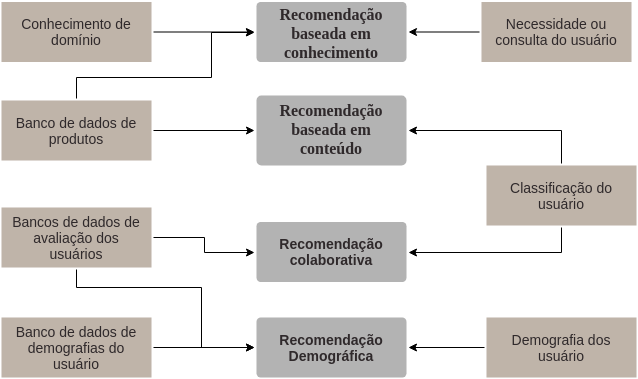
\includegraphics[width=.8\textwidth]{figuras/secao-referencial/tecnicasRecomendacao.png}
\caption{Técnicas de Recomendação e fontes de conhecimento. Adaptado de \cite{burke2007hybrid}.}
\label{img:recomendacao}
\end{figure}



\section{Considerações Finais do Capítulo}

Há indícios de que o perfil do testador possua interferência nas atividades de teste. Os testes realizados acerca dos serviços que chegam ao ITRAC fazem parte de um contexto propenso a se realizar estudos que envolvem os temas abordados neste capítulo de Referencial Teórico.

A partir do conteúdo obtido com a pesquisa bibliográfica especificada em \ref{ch:metodologia} e apresentado neste capítulo, este trabalho busca aplicar conceitos relacionados a perfis de testadores, utilizando de técnicas de trabalhos já publicados sobre sistemas de recomendação, a fim de realizar uma adaptação para consolidação da abordagem discutida no Capítulo~\ref{ch:proposta}. 

% \del{Verifique o parágrafo acima}
% \chapter{Proposta do Trabalho}
\label{ch:proposta}

\section{Considerações Iniciais}

// o volume atual de testes feitos pelo ME. 

Dado o objetivo deste trabalho, o presente capítulo retoma o plano metodológico adotado apresentado no Capítulo \ref{ch:metodologia} e apresenta um detalhamento das atividades já realizadas e as atividades a serem realizadas. 

O detalhamento será descrito quanto às fases de \textit{Planejamento da Pesquisa} e da \textit{Coleta de Dados}, que representam os procedimentos e técnicas utilizados para a consolidação da proposta deste trabalho. Finalizando, apresenta-se o cronograma de execução das atividades a serem realizadas para a conclusão do trabalho.

\section{Atribuição de Casos de Teste Baseado no Perfil de Testadores}

A pesquisa bibliográfica realizada colaborou para a construção da proposta deste trabalho de se realizar uma abordagem para atribuição dinâmica de atividades de teste com base no perfil dos testadores envolvidos no time de testes do ITRAC. 

Cada etapa apresentada neste capítulo consolida uma fase da parte prática deste trabalho, que será executada no TCC2. Para se realizar a elicitação, análise e modelagem dos requisitos para o sistema de recomendação, selecionou-se o procedimento de pesquisa-ação para realização das
atividades de forma participativa e interativa entre pesquisador e membros do objeto de estudo.

Sendo assim, para esta pesquisa, relacionam-se e entendem-se as seguintes etapas:

\begin{enumerate}
    \item Identificação e levantamento de características pessoais que podem influenciar o processo de teste de software no contexto apresentado;

    \item Extração de informações sobre as características pessoais de cada testador envolvido no processo de teste;

    \item Acompanhamento do processo de teste de um serviço fictício criado com diferentes características, registrando métricas que viabilizam a análise da adequação entre tours e testadores específicos;

    % \item Acompanhamento do processo de teste de diversos serviços, com diferentes características, registrando métricas que viabilizam a análise da adequação entre tipos de teste e testadores específicos;

    \item Análise dos dados registrados sobre o teste;

    \item Definição de \textit{Sistema de Recomendação} que se baseia no conjunto de dados registrados sobre o teste no serviço fictício para recomendar casos de teste para testadores;

    \item Proposição de uma estratégia de filtragem para ponderar futuras recomendações, levando em consideração a satisfação do testador durante a realização das atividades de teste.
\end{enumerate}


As Seções \ref{sec:caracteristicas_importantes}, \ref{sec:extrair_caracteristicas}, \ref{sec:acompanhar_ciclos} e \ref{sec:analisar_dados} apresentam as técnicas de coleta de dados e relaciona as principais etapas da abordagem proposta neste trabalho.

\section{Características de Perfil}
\label{sec:caracteristicas_importantes}

A técnica de \textit{Observação}, proposta como técnica de coleta de dados em uma das fases da metodologia adotada, foi empregada neste trabalho a partir do estudo sobre a equipe objeto de estudo.

Como já apresentado no Capítulo \ref{ch:referencial}, na Seção \ref{sec:perfil_testadores}, a influência da personalidade humana em tarefas individuais é uma das preocupações da Engenharia de Software.  Sendo assim, a influência da personalidade também é uma característica importante deste trabalho, pois configura o mecanismo principal para realização da Atribuição dos casos de teste dinamicamente.

A equipe de testadores do ITRAC possui membros com níveis variados de experiência em testes, sendo composta por alunos graduandos em Engenharia de Software, que cursam períodos diferentes do curso, podendo variar entre calouros e veteranos. Além disso, parte da equipe que realiza os testes nos serviços, utilizando o processo de testes definido pelo ITRAC, é composta por funcionários do ME, já graduados em diferentes cursos, que podem possuir, ou não, uma maior experiência em testes, de um modo geral.

Esta variação entre os membros da equipe e seus respectivos conhecimentos não é considerada no momento da Atribuição de tarefas de teste realizadas. Sendo assim, alunos que estão no início da graduação e sem nenhuma experiência em testes, podem ser alocados a tarefas de teste que possuem o mesmo nível de dificuldade de tarefas de teste alocadas a testadores experientes.

Esta falta de critério na Atribuição de tarefas de teste pode gerar prejuízos ao processo de Validação do produto de software. Este problema é atacado no trabalho atual, objetivando uma melhor adequação entre os testadores e as tarefas teste realizadas.

\section{Extração de Informações de Perfil}
\label{sec:extrair_caracteristicas}

Neste trabalho, é necessário extrair as informações sobre o perfil de cada testador da equipe do ITRAC. A extração de informações é feita a partir da \textit{técnica de Coleta de Dados Questionário}. O Questionário foi desenvolvido com base em~\cite{Santos19SDPA}, \cite{geras2004survey} e~\cite{groves2000survey} e é apresentado no Anexo~\ref{anexo:questionario}.

A criação do questionário foi baseada nas  diretrizes de Kitchenham~\cite{kitchenham2008personal} que apresenta 6 etapas a serem realizadas, como ilustrado na Figura~\ref{fig:Abordagem}.

        \begin{figure}[h]
          \centering
          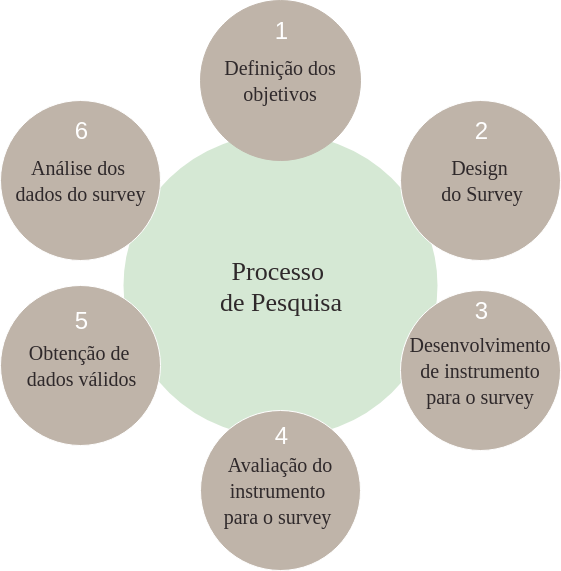
\includegraphics[width=10cm]{figuras/survey.png}
          \caption{Visão geral do processo para elaboração do questionário.  (Fonte: Elaborado pela Autora.)}
          \label{fig:Abordagem}

        \end{figure}

As 6 etapas estão sendo empregadas neste, conforme descrição a seguir:

\begin{enumerate}
\item \textbf{Estabelecer objetivos:} neste trabalho, esta etapa configura o primeiro passo para começar a construir o questionário. Em que cada objetivo é definido;

\item \textbf{Design do \textit{survey}:} o tipo de \textit{design} utilizado neste trabalho é o transversal~\cite{geras2004survey}, no qual os participantes serão questionados sobre suas experiências prévias;

\item \textbf{Desenvolvimento de instrumento para o \textit{survey}:} para desenvolver o instrumento, foram empregados os passos: (i) pesquisar a literatura relevante (apresentada no Capítulo~\ref{ch:referencial}); (ii) construir um instrumento (Capítulo~\ref{ch:metodologia}); (iii) avaliar o instrumento (em produção); e (iv) documentar o instrumento (redação do trabalho como um todo);

\item \textbf{Avaliação do instrumento para o \textit{survey}:} esta avaliação é frequentemente chamada de pré-teste, e possui objetivos distintos: (i) verificar se as questões são compreensíveis; (ii) avaliar a taxa de resposta provável e a eficácia dos procedimentos de acompanhamento; (iii) avaliar a confiabilidade e validade do instrumento; e (iv) garantir que nossa análise de dados as técnicas correspondem às nossas respostas esperadas;

\item \textbf{Obtenção de dados válidos:} nesta fase é definida uma amostra, que é um subconjunto da população. As respostas deste grupo buscam representar o grupo inteiro. Ao escolher a amostra a ser pesquisada, devemos ter em mente três aspectos do desenho da pesquisa: (i) evitar o viés; (ii) adequação; e (iii) custo-efetividade;

\item \textbf{Análise dos dados do \textit{survey}:} na etapa final, são reunidos todos os dados coletados da pesquisa para extrair informações relevantes para responder às questões definidas nos objetivos da pesquisa e descritas no GQM, destacado na Tabela~\ref{tab:gqm}.
\end{enumerate}

Para este trabalho de conclusão de curso (TCC1), foram realizados as 2 primeiras etapas e parte da terceira. O restante das etapas configuram parte do trabalho a ser realizado no TCC2.

\subsection{Design e Questões do Questionário}
\label{sec:desingquestions}

Para projetar o questionário buscou-se na literatura trabalhos similares.

O questionário foi elaborado tomando como base outros artigos que realizavam este tipo de pesquisa, por exemplo, o \textit{survey} de~\cite{geras2004survey}, que descreveu os resultados de um \textit{survey} de questionamentos feitos à pessoas envolvidas com o desenvolvimento de software em uma empresa. A partir disso, com o objetivo de caracterizar testes de software e práticas de garantia da qualidade, o questionário foi dividido nas seguintes categorias:

Exemplo \cite{model1980multiprocessing}

\begin{itemize}
\item  Perfil pessoal e profissional dos respondentes;
\item  Conhecimentos específicos de teste; e
\item  Relato livre de experiência.
\end{itemize}

As perguntas referentes à cada categoria podem ser consultadas no Anexo~\ref{anexo:questionario}.

A primeira categoria foi elaborada com o objetivo de coletar informações pessoais e sobre o perfil profissional do respondente, com o interesse em entender o nível de escolaridade, respectivos cursos de graduação, experiências com linguagens de programação e para coletar os usuários de cada testador na ferramenta de gerenciamento de projetos utilizada. No contexto desta pesquisa, foi utilizada a ferramenta \textit{redmine}\footnote{https://www.redmine.org/}.

A segunda categoria busca entender o grau de familiaridade dos testadores com a atividade de teste. Para isto, o questionário aborda questões sobre técnicas e critérios de teste, por exemplo, para entender como é a experiência dos testadores neste quesito.


A terceira categoria engloba uma questão aberta, que solicita ao testador que relate a sua experiência. Esta questão se faz importante, pois as respostas serão fundamentais para que o testador relate livremente sua experiência, podendo incluir informações que o questionário ainda não contém, mas que são relevantes para a pesquisa. Podendo colaborar, dessa forma, com o aprimoramento do questionário.

É interessante ressaltar que o questionário ainda está em fase de construção e será aprimorado após uma primeira aplicação com um membro do ITRAC, que fará parte da equipe de testes dos serviços.

\section{Acompanhar Ciclos}
\label{sec:acompanhar_ciclos}

Para se utilizar dados necessário para o desenvolvimento do sistema, foi utilizada uma estratégia de registro de informações que envolve 4 etapas propostas por \cite{petersen2008systematic}, apresentada na Subseção~\ref{sub:pesquisa-acao} e ilustrada na Figura~\ref{fig:etapasPesquisaAcaoAdotas}.

        \begin{figure}[!htb]
          \centering
          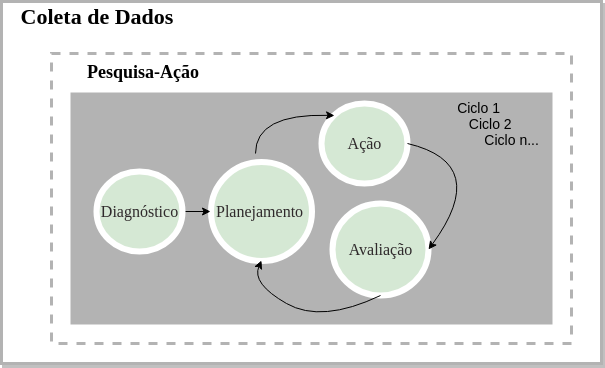
\includegraphics[width=12cm]{figuras/etapasPesquisaAcao.png}
          \caption{Etapas da estratégia de Pesquisa-Ação adotada. (Fonte: Elaborado pela Autora.)}
          \label{fig:etapasPesquisaAcao}

        \end{figure}

Na fase de \textit{Diagnóstico}, buscou-se entender o processo que os testadores seguem para descobrir como seriam feitos os registros de determinadas informações. Estas informações necessárias são apresentadas, também, na Tabela~\ref{tab:gqm}, que será apresentada mais à frente. A partir disso, foi feita a construção de um fluxo, apresentado na Figura~\ref{fig:fluxo}, que deve ser seguido até que se inicie o desenvolvimento do sistema de recomendação.

        \begin{figure}[!htb]
          \centering
          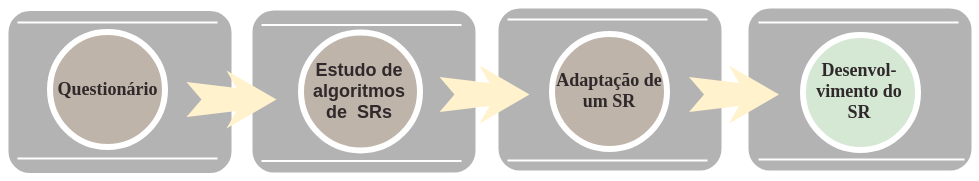
\includegraphics[width=16cm]{figuras/fluxo.png}
          \caption{Fluxo para desenvolvimento do SR.  (Fonte: Elaborado pela Autora.)}
          \label{fig:fluxo}

        \end{figure}

Com o objetivo de facilitar o entendimento das funcionalidades do sistema, apresentar um protótipo e validá-lo com a equipe do ITRAC, serão empregados alguns ciclos. Os ciclos serão desenvolvidos no TCC2.

O acompanhamento de ciclos deve levar em consideração o registro de determinadas informações. Para tanto, foi necessária a elaboração de um \textit{Goal Question Metric - GQM}, que consiste em um mecanismo utilizado para definir e avaliar um conjunto de objetivos operacionais, utilizando um conjunto de questões e métricas associadas a estes objetivos~\cite{basili1994goal}. O GQM desta pesquisa é apresentado na Tabela~\ref{tab:gqm}:

% Please add the following required packages to your document preamble:
% \usepackage[table,xcdraw]{xcolor}
% If you use beamer only pass "xcolor=table" option, i.e. \documentclass[xcolor=table]{beamer}
\begin{table}[htb!]
\caption{\textit{Goal Question Metric} (GQM).}
\label{tab:gqm}
\begin{tabular}{|l|l|}
\hline
\rowcolor[HTML]{C0C0C0}
\textbf{Goal} & \begin{tabular}[c]{@{}l@{}}Aprimorar o gerenciamento de testes para a atribuição de \\ tarefas de teste com base no perfil do testador\end{tabular} \\ \hline
\rowcolor[HTML]{FFFFFF}
\textbf{Question 1} & Qual a eficiência da Atribuição de tarefas de teste para a equipe? \\ \hline
\rowcolor[HTML]{FFFFFF}
\textbf{Métricas} & \begin{tabular}[c]{@{}l@{}}M1: Número de casos de teste gerados pela equipe\\ \\ M2: Número de falhas identificadas pela equipe\\ \\ M3: M2/M1\end{tabular} \\ \hline
\rowcolor[HTML]{EFEFEF}
\textbf{Question 2} & Qual a eficiência da Atribuição de casos de teste por parte do testador? \\ \hline
\rowcolor[HTML]{EFEFEF}
\textbf{Métricas} & \begin{tabular}[c]{@{}l@{}}M1: Número de casos de teste gerados pelo testador\\ 		\\ M4: Número de falhas identificadas por testador\\ 		\\ M5: M4/M3\end{tabular} \\ \hline
\rowcolor[HTML]{FFFFFF}
\textbf{Question 3} & Qual o impacto do perfil do testador na eficiência dos testes? \\ \hline
\rowcolor[HTML]{FFFFFF}
\textbf{Métrica} & M5: Variação entre a eficiência de cada testador \\ \hline
\rowcolor[HTML]{EFEFEF}
\textbf{Question 4} & Qual o grau de satisfação do testador durante o ciclo de teste? \\ \hline
\rowcolor[HTML]{EFEFEF}
\textbf{Métrica} & M6: Grau de satisfação (0 a 5) \\ \hline
\rowcolor[HTML]{FFFFFF}
\textbf{Question 5} & Qual a eficiência dos testes em relação a cada tour? \\ \hline
\rowcolor[HTML]{FFFFFF}
\textbf{Métrica} & M6 (tour 1) = M1(tour 1)/M4(tour1) \\ \hline
\end{tabular}
\end{table}

Dadas as etapas destacadas, a Seção~\ref{sec:abordagem} apresenta a abordagem proposta neste trabalho.

\section{Abordagem}
\label{sec:abordagem}

A abordagem proposta nesta pesquisa envolve um processo contínuo de aprendizado e evolução, que depende de diversos ciclos de teste em diferentes tipos de serviço. O contexto no qual o laboratório ITRAC se encontra viabiliza a aplicação de tal abordagem, dada as características de um processo de transformação digital em grande escala.

O processo de transformação digital do governo brasileiro envolve um grande número de serviços de baixa complexidade, o que possibilita um grande número de ciclos de teste em um curto período de tempo. Tal característica favorece o aprendizado e a evolução relacionada as atividades de teste neste contexto.

A partir das métricas destacadas na Tabela~\ref{tab:gqm}, é possível que análises sejam realizadas buscando uma melhora contínua da atividade de Atribuição de casos de teste.

Neste sentido, a Figura~\ref{fig:Abordagem} apresenta o processo contínuo de aprendizado, juntamente com a abordagem proposta para este trabalho. Foi utilizado o \textit{lemniscate} -- figura do número 8 virada para representar o processo.

        \begin{figure}[h]
          \centering
          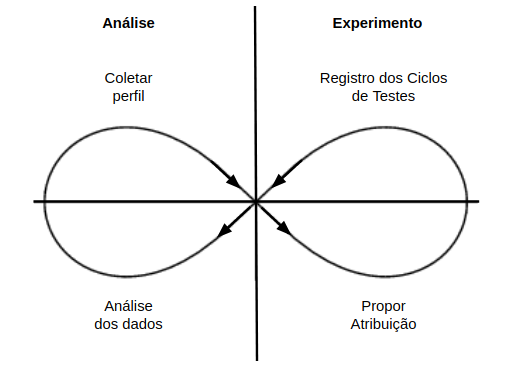
\includegraphics[width=13cm]{figuras/abordagem.png}
          \caption{Abordagem para o Sistema de Recomendação  (Fonte: Elaborado pela Autora.)}
          \label{fig:Abordagem}

        \end{figure}


A parte esquerda da figura relaciona-se com a Análise e está vinculada à coleta do perfil do testador e à análise dos dados coletados depois de cada ciclo de teste. Enquanto a parte direita relaciona o que se pretende usar como experimento, que configura o registro dos ciclos de teste e a proposta de Atribuição. A seguir, serão descritas cada fase da abordagem:

\subsection{Coletar Perfil}

% Perfil será coletado a partir dos alunos das disciplinas de Testes de Software e de Software Experimental

Como apresentado na Seção~\ref{sec:caracteristicas_importantes}, as características de perfil de cada testador serão levadas em consideração para a constituição deste trabalho. Para dar início às partes práticas será necessário coletar o perfil dos testadores envolvidos. O perfil de cada testador será traçado a partir da extração de informações do perfil obtidas a partir do questionário já apresentado na Seção \ref{sec:extrair_caracteristicas}.

O questionário será refinado até estabelecer as questões necessárias para consolidar um perfil que contenha as informações necessárias do usuário sobre cada categoria apresentada na Subseção \ref{sec:desingquestions}. Após a consolidação deste perfil, uma página de perfil para cada testador será criada na ferramenta \itractool para que os testadores tenham um cadastro com todas as informações coletadas.

\subsubsection{Cadastrar perfil na ferramenta \itractool}

É importante que os testadores tenham seus perfis individuais cadastrados na ferramenta, pois estes perfis irão fornecer a informação sobre o domínio dos testadores sobre testes. Estas informações serão registradas no banco de dados e serão atualizadas de acordo com a realização dos cilos de teste.

Com as informações cadastradas será possível traçar, baseado em dados históricos, qual a tarefa de teste ou o \textit{tour} mais adequado para cada perfil de testador, levando em consideração a experiência do testador com o teste exploratório dos serviços. A partir disso, será possível predizer quais atividades de teste ele está executando com mais eficiência para poder realizar uma melhor Atribuição de atividades de teste. O perfil ideal para o testador seria aquele que conseguisse captar além das características técnicas, a experiência naquele domínio de aplicação para, em seguida, propor uma Atribuição.

\subsection{Propor Atribuição}

 Esta fase consiste na proposta de Atribuição baseada em perfil, ou seja, uma página de um serviço com determinados campos e características específicas pode ter um caso de teste e um testador ideal. O sistema de recomendação sugere quais \textit{tours} são adequados para determinado testador utilizar baseado em seu histórico de testes já realizados. A partir disso, a página e campos em questão são testados.

 Os sistemas de recomendação, como já explicitado no Capítulo \ref{ch:referencial}, na Seção \ref{sec:sistemas}, realizam filtragens de informações que recomendam itens aos usuários. No caso deste trabalho o item é uma Atribuição de \textit{tours} para um testador.

É importante destacar que a execução de um \textit{tour} por parte de um testador, dá origem a um conjunto de teste, gerado a partir do \textit{tour}. A Atribuição de \textit{tours} e testadores deve ser realizada de maneira dinâmica, com um processo de aprendizado durante cada ciclo de teste. Ou seja, a Atribuição dos \textit{tours} e dos testadores deve levar em consideração, além das características já citadas, o aprendizado obtido ao longo dos ciclos de teste anteriores. O aprendizado citado busca maximizar a eficiência da aplicação dos casos de teste. Neste contexto, a palavra ``eficiência'' faz referência a taxa de identificação de falhas durante a aplicação dos casos de teste. Desse modo, a ``eficiência'' é dada pela Equação \ref{eq:eficiencia}.

 \begin{equation}
 \label{eq:eficiencia}
    eficiência = \frac{numero \ de \ falhas\ identificadas}{numero\ de\ casos\ de\ teste\ do\ tour}
 \end{equation}


% \del{Aqui achei que ficou um pouco estranho. Acho que para clarear, precisava falar que, a execução de um tour por parte de um testador, dá origem a um conjunto de teste, gerado a partir do tour. Ai dá para entender que há uma relacionamento entre caso de teste, tour e testador.}

Neste trabalho, assim como proposto em~\cite{miranda2012recommender}, a Atribuição é representada como um par conjunto de teste e testador, representado por \{CTn;Tn\} (Caso de Teste \emph{n} e Testador \emph{n}). O usuário é representado por um típico gerente de teste e as recomendações são feitas comparando um caso de teste específico com o perfil de um testador e avaliando sua similaridade.

Após a Atribuição e a realização dos casos de teste alocados, surge a etapa de registro dos casos de teste, detalhada a seguir.

\section{Registro dos Ciclos de Teste}

Os casos de teste realizados pelos testadores do ITRAC já são registrados na ferramenta \textit{Redmine}. Estes casos de teste já possuem um padrão a ser seguido para terem suas informações guardadas. Com isso, a obtenção dos casos de teste realizados pode ser feita a partir da API (\textit{Application Programming Interface}) do \textit{Redmine}.

A Figura \ref{fig:registro} apresenta a estrutura organizacional atual dos registros realizados no \textit{Redmine}.


        \begin{figure}[h]
          \centering
          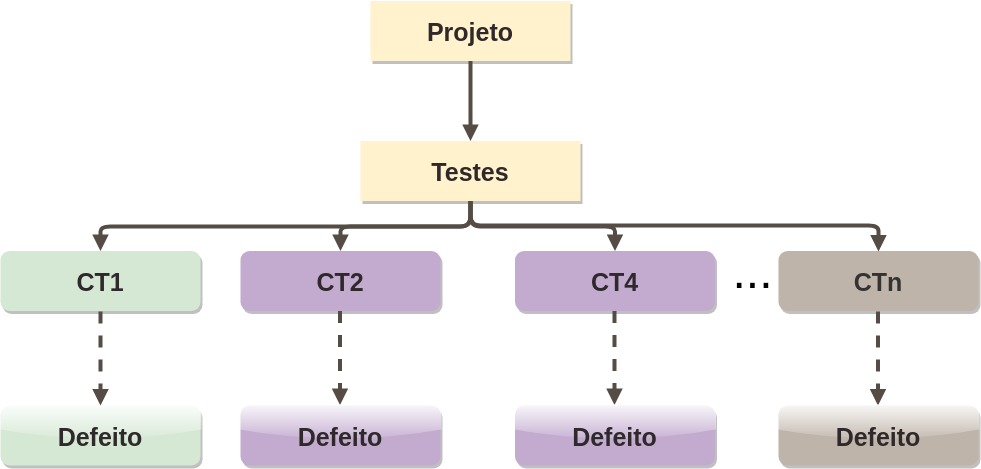
\includegraphics[width=15cm]{figuras/registro.png}
          \caption{Estrutura Organizacional dos Registros no \textit{Redmine}. (Fonte: Elaborado pela Autora.)}
          \label{fig:registro}

        \end{figure}

Na Figura \ref{fig:registro}, \textbf{Projeto} representa um serviço digitizado, que foi registrado no \textit{Redmine}. \textbf{Testes} representam o conjunto de casos de teste associados ao projeto. O conjunto de testes é definido à partir do conceito de \textit{tasks} do \textit{Redmine}. A definição desta entidade que agrupa os casos de teste se deu para facilitar a obtenção de informações de maneira agrupada, viabilizando, por exemplo, a extração do status de conclusão do conjunto de casos de teste como um todo.

Os \textbf{CTs} representam os casos de teste registrados no \textit{Redmine}. Estes são definidos a partir do conceito de \textit{subtasks} associados à \textit{task} \textbf{Testes} e possuem os atributos apresentados na Tabela \ref{tab:atributo}.

% Please add the following required packages to your document preamble:
% \usepackage[table,xcdraw]{xcolor}
% If you use beamer only pass "xcolor=table" option, i.e. \documentclass[xcolor=table]{beamer}
\begin{table}[H]
\centering
\caption{Atributos dos Casos de Teste Registrados no \textit{Redmine}.}
\label{tab:atributo}
\begin{tabular}{|l|l|}
\hline
\textbf{Atributo} & \textbf{Descrição} \\ \hline
Título & Registra o título do caso de teste \\ \hline
\rowcolor[HTML]{EFEFEF}
Data de criação & Registra a data de criação do teste \\ \hline
Data de execução & Registra a data da execução do teste \\ \hline
\rowcolor[HTML]{EFEFEF}
Tempo para execução & \begin{tabular}[c]{@{}l@{}}Registra o tempo gasto para realizar \\ o caso de teste\end{tabular} \\ \hline
Tour utilizada & Registra a tour utilizada para o caso de teste \\ \hline
\rowcolor[HTML]{EFEFEF}
\begin{tabular}[c]{@{}l@{}}Quantidade de \\ campos envolvidos\end{tabular} & \begin{tabular}[c]{@{}l@{}}Registra quantos campos estão envolvidos\\  no caso de teste\end{tabular} \\ \hline
Testador responsável & \begin{tabular}[c]{@{}l@{}}Registra o testador responsável pela execução\\ do caso de teste\end{tabular} \\ \hline
\rowcolor[HTML]{EFEFEF}
Resultado & \begin{tabular}[c]{@{}l@{}}Registra o resultado final da execução do\\ caso de teste (sucesso, ou falha)\end{tabular} \\ \hline
Entrada & Registra as entradas aplicadas ao caso de teste \\ \hline
\rowcolor[HTML]{EFEFEF}
Saída esperada & Registra a saída esperada para o caso de teste \\ \hline
Saída obtida & \begin{tabular}[c]{@{}l@{}}Registra a saída obtida durante a aplicação\\ do caso de teste\end{tabular} \\ \hline
\rowcolor[HTML]{EFEFEF}
Descrição & Registra a descrição do caso de teste \\ \hline
\end{tabular}
\end{table}

Os \textbf{Defeitos} são definidos como \textit{subtasks} das \textit{subtasks} \textbf{CTs} e possuem os atributos apresentados na Tabela \ref{tab:defeito}. Vale ressaltar que os \textbf{CTs} podem possuir, ou não, um \textbf{Defeito} associado. Essa possibilidade de ter ou não um Defeito associado é representado, na Figura \ref{fig:registro}, a partir da utilização de setas trastejadas.

% Please add the following required packages to your document preamble:
% \usepackage[table,xcdraw]{xcolor}
% If you use beamer only pass "xcolor=table" option, i.e. \documentclass[xcolor=table]{beamer}
\begin{table}[H]
\centering
\caption{Atributos dos Defeitos Registrados no \textit{Redmine}.}
\label{tab:defeito}
\begin{tabular}{|l|l|}
\hline
\textbf{Atributo} & \textbf{Descrição} \\ \hline
\rowcolor[HTML]{FFFFFF}
Título & Registra o título do defeito \\ \hline
\rowcolor[HTML]{EFEFEF}
Prioridade & Registra o nível de prioridade para a resolução do defeito \\ \hline
\rowcolor[HTML]{FFFFFF}
Categoria & Registra a categoria a qual o defeito pertence \\ \hline
\rowcolor[HTML]{EFEFEF}
Tipo de falha & Registra o tipo de falha encontrada \\ \hline
\rowcolor[HTML]{FFFFFF}
\begin{tabular}[c]{@{}l@{}}Passos para \\ reproduzir o bug\end{tabular} & Registra os passos que levaram à ocorrência da falha \\ \hline
\rowcolor[HTML]{EFEFEF}
Provas visuais & \begin{tabular}[c]{@{}l@{}}Registra os defeitos encontrados, geralmente, em forma \\ de \textit{prints}, como prova visual\end{tabular} \\ \hline
\rowcolor[HTML]{FFFFFF}
Ambiente & \begin{tabular}[c]{@{}l@{}}Registra em qual sistema operacional, resolução da tela,\\ browser e nível de zoom o a falha ocorreu\end{tabular} \\ \hline
\end{tabular}
\end{table}

Em relação ao atributo \textbf{Tipo de Falha}, vale destacar que os tipos definidos até o momento são: 1) Regra de Negócio, 2) Interface e 3) Validação de Campos.

\section{Análise dos Dados}
\label{sec:analisar_dados}

Com base na análise do GQM, a intenção é verificar a existência de uma correlação entre a eficiência no processo de teste e as diferentes variáveis que compõem o perfil dos testadores. Este perfil será identificado com base em diferentes questões respondidas pelos testadores num questionário digital, como o apresentado no Anexo~\ref{anexo:questionario}.

Ao obter as questões respondidas do questionário, o passo seguinte é coletar os dados sobre a eficiência de cada testador na realização das atividades de teste. Para que se colete estes dados, é possível a realização de testes de correlação para identificar se há alguma relação entre as variáveis do perfil e a eficiência nos testes de determinado testador ou da equipe de testes como um todo.

Baseado nos dados, pode-se retomar à pergunta de pesquisa e entender: \textbf{Qual o impacto das variáveis do perfil do testador na eficiência dos testes?} A partir desta fase, é possível utilizar o questionário para fazer um teste de correlação entre as variáveis levantadas.


\section{Integração \itractool}

Este trabalho propõe a inclusão de um novo módulo na ferramenta \itractool, apresentada na Seção \ref{sec:dtest}. A integração deste módulo segue o apresentado na Figura \ref{img:architecture2}.

\begin{figure}[!htb]
  \centering
  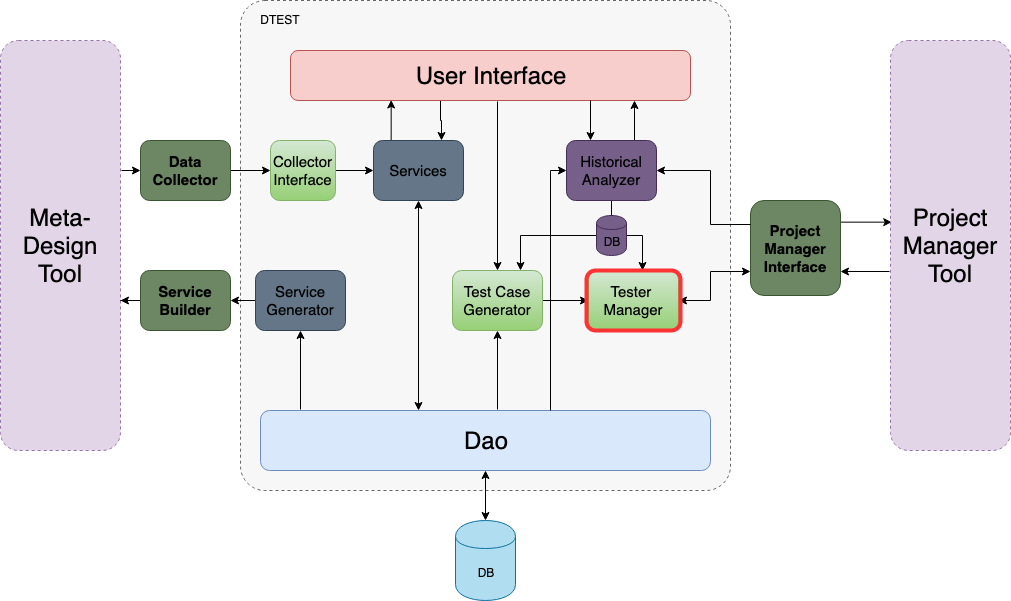
\includegraphics[width=14cm]{figuras/arquitetura.png}
  \caption{Arquitetura \itractool após a inclusão do módulo \textit{Tester Manager}.)}
  \label{img:architecture2}
\end{figure}

O módulo proposto, chamado de \textbf{Tester Manager}, utiliza como \textit{input} informações advindas dos módulos \textbf{Test Case Generator} (TCG) e \textbf{Historical Analyzer} (HA), além de informações diretamente obtidas a partir da ferramenta de gerenciamento de projetos utilizada.

O módulo TCG exporta o caso de teste que deverá ser alocado entre os testadores disponíveis. O módulo \textbf{Tester Manager}, com base nas informações de perfil de cada testador, deverá associar o testador que mais se adéqua ao caso de teste em questão. Para isso, informações histórias da execução de casos de teste são utilizadas como base de conhecimento. Um processo de aprendizado utilizando esta base de conhecimento viabiliza a implementação de um \textit{Sistema de Recomendação} que seja capaz de recomendar o testador mais adequado para determinado caso de teste.


\section{Cronograma}

A Figura \ref{fig:cronograma} apresenta o cronograma de atividades do Trabalho de conclusão de Curso. Desde as atividades já realizadas durante o TCC1 até a concretização do sistema de recomendação, prevista para ser desenvolvida no TCC2.

Na Figura \ref{fig:cronograma}, a cor destacada em verde representa as atividades já desenvolvidas, considerando o término do TCC 1. Em amarelo, as atividades a serem desenvolvidas.

        \begin{figure}[H]
          \centering
          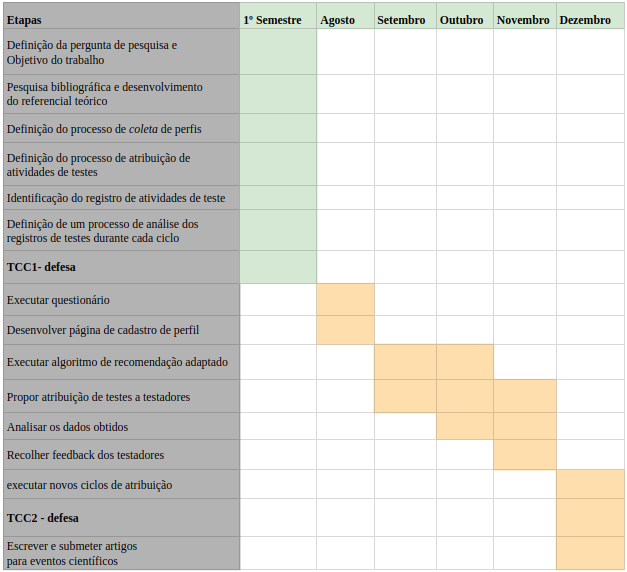
\includegraphics[width=15cm]{figuras/cronograma.png}
          \caption{Cronograma (Fonte: Elaborado pela Autora.)}
          \label{fig:cronograma}

        \end{figure}

\section{Considerações Finais do Capítulo}
\label{sec:final-cap}

Analisando o contexto no qual o ITRAC está inserido é possível perceber um ambiente propício para a aplicação da abordagem proposta, visto que já existe uma ferramenta sobre testes em desenvolvimento. A integração de um módulo que proponha a atribuição dos casos de teste é viável nesta equipe se considerarmos as informações obtidas a partir da ferramenta.

Enquanto os demais capítulos sintetizaram o \textit{background} para a realização deste trabalho, o presente capítulo buscou apresentar a abordagem proposta para este trabalho. Detalhada e apresentada em modelo e de arquitetural. 

Espera-se que no TCC2 o desenvolvimento desta ferramenta seja concretizado e colocado em uso para os testadores do ITRAC. 

\chapter{Materiais e Métodos}
\label{ch:metodologia}
\section{Considerações Iniciais}
Neste capítulo apresentam-se a classificação da pesquisa e o plano metodológico adotado para o alcance do objetivo desta pesquisa, isto é: \textit{Obter perfis de testadores utilizando características e experiência do domínio para Atribuição automática de tarefas de teste, utilizando a equipe de transformação de serviços do governo do ITRAC - Information Technology and Application Center}.

Assim, apresenta-se o planejamento metodológico em fases e atividades.Seguido do diagnóstico do objeto de estudo.

\section{Plano Metodológico Adotado}
\label{sec:planMetodologico}

O plano metodológico adotado neste trabalho compreende quatro fases básicas: planejamento da pesquisa; coleta de dados; análise dos dados; e relato dos resultados, como apresentado  na Figura \ref{fig:PlanoGeral} abaixo:

        \begin{figure}[H]
          \centering
          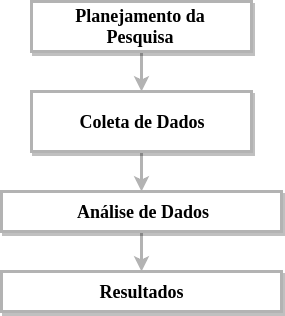
\includegraphics[width=6cm]{figuras/planoGeral.png}
          \caption{Plano metodológico adotado (Fonte: Elaborado pela Autora.)}
          \label{fig:PlanoGeral}

        \end{figure}

O trabalho foi desenvolvido no contexto do laboratório ITRAC, junto ao time de testadores envolvidos nos testes dos serviços transformados para o ME. Sendo assim, o objeto de estudo é o\textit{ time de testadores do ITRAC}.

Na fase de coleta de dados os procedimentos de pesquisa empregados foram: pesquisa documental; pesquisa bibliográfica; e a prototipação. Um questionário foi elaborado para aplicação futura dentre os membros da equipe de teste.

Nas subseções caracterizadas pelas fases do plano metodológico são apresentadas juntamente com uma descrição de cada um dos procedimentos empregados, como apresentado na Figura \ref{fig:fasesPlano}.


        \begin{figure}[H]
          \centering
          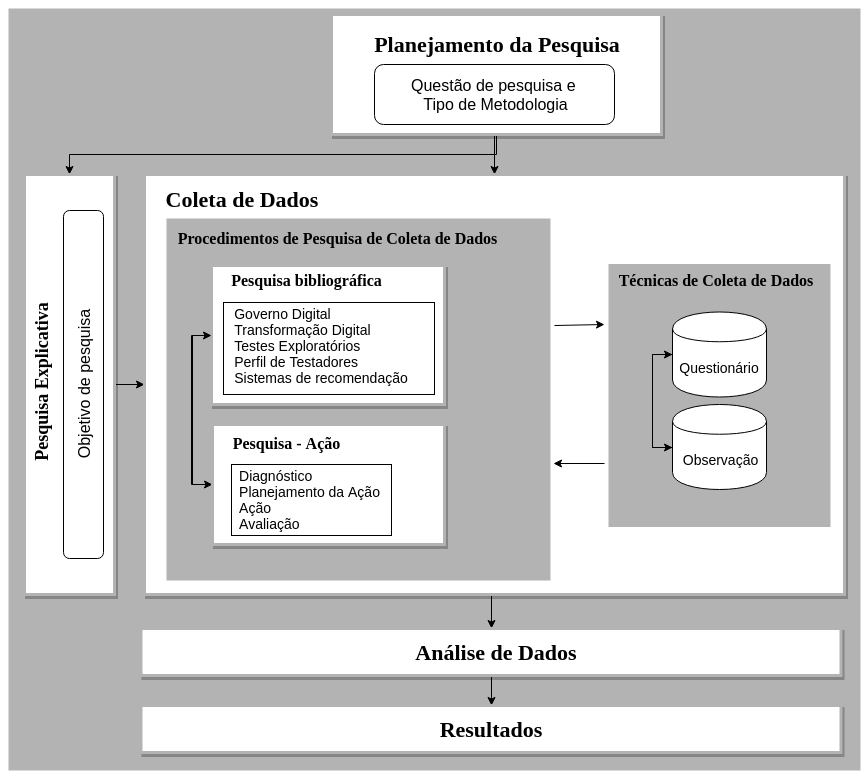
\includegraphics[width=16cm]{figuras/fasesPlanoMetodologico.png}
          \caption{Fases do Plano Metodológico adotadas nesta pesquisa. (Fonte: Elaborado pela Autora.)}
          \label{fig:fasesPlano}

        \end{figure}


\subsection{Fase de Planejamento da Pesquisa}

Na fase de Planejamento da Pesquisa foi configurada a elaboração de todo o Capítulo \ref{ch:introducao} de Introdução. Foi definido o tema de pesquisa, pergunta de pesquisa, objetivos e, também, definição e classificação metodológica.

A Figura \ref{fig:PlanPesquisa} apresenta esta fase importante para as definições iniciais da pesquisa.

        \begin{figure}[H]
          \centering
          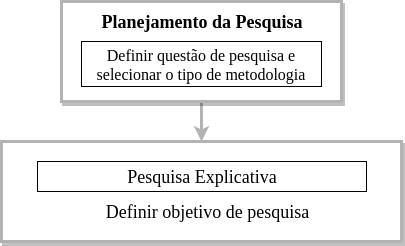
\includegraphics[width=6.5cm]{figuras/planejamentoPesquisa.png}
          \caption{Planejamento da pesquisa. (Fonte: Elaborado pela Autora.)}
          \label{fig:PlanPesquisa}

        \end{figure}


        % \begin{figure}[H]
        %   \centering
        %   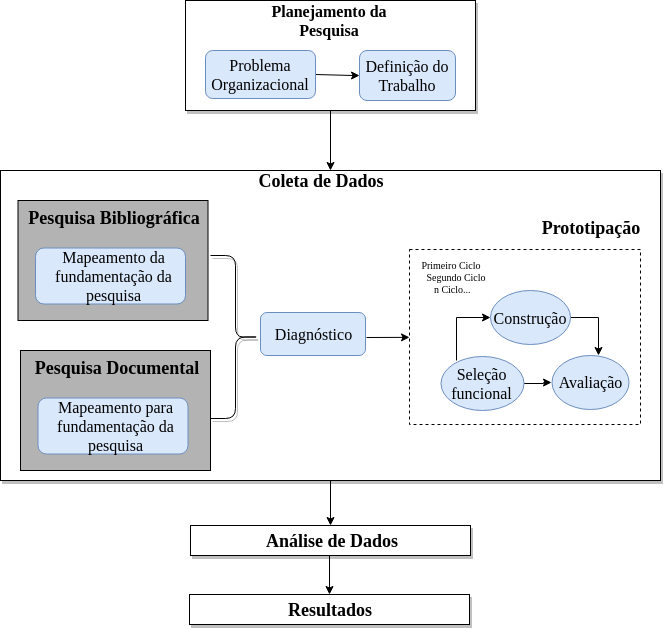
\includegraphics[width=14cm]{figuras/planoMetodologico.png}
        %   \caption{Plano metodológico adotado (Fonte: Elaborado pela Autora.)}
        %   \label{fig:PlanoMetodologico}

        % \end{figure}

\subsection{Fase de Coleta de Dados}

A fase de coleta de dados configurou o recolhimento de boa parte do conteúdo necessário para a consolidação deste trabalho, foram adotados os procedimentos de \textit{pesquisa bibliográfica} e adotados os procedimentos da \textit{pesquisa - ação}.

A Figura \ref{fig:coletaDados} apresenta os procedimentos de coleta de dados e as técnicas adotadas para o presente trabalho.

        \begin{figure}[H]
          \centering
          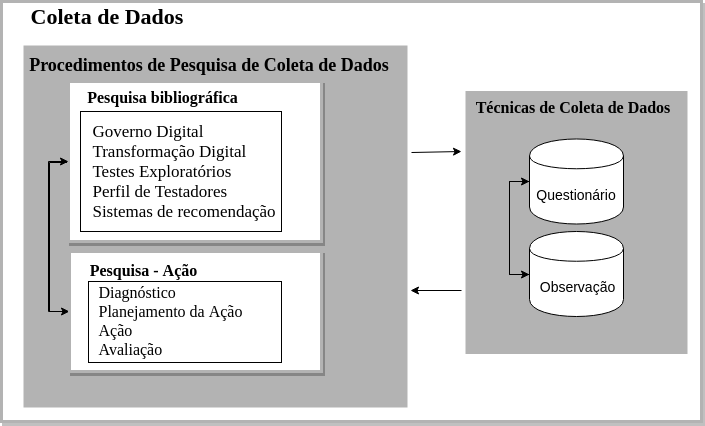
\includegraphics[width=10cm]{figuras/coletadeDados.png}
          \caption{Coleta de Dados. (Fonte: Elaborado pela Autora.)}
          \label{fig:coletaDados}

        \end{figure}

A análise bibliográfica permitiu com que fosse recolhido embasamentos relevantes sobre os temas relacionados a esta pesquisa. Algumas atividades da pesquisa-ação já realizadas também promoveram uma iteração maior entre pesquisados e equipe do objeto de estudo do laboratório.

\subsection{Pesquisa Bibliográfica}

A partir da pesquisa bibliográfica foi possível recolher embasamentos relevantes sobre Governo Digital, Transformação Digital, Testes Exploratórios, Perfil de Testadores e Sistemas de Recomendação. Cada um dos embasamentos sobre os temas coletados foram apresentados no Capítulo \ref{ch:referencial} de Referencial Teórico.

\subsection{Fase de Pesquisa-Ação}
\label{sub:pesquisa-acao}

A estratégia de Pesquisa-Ação neste trabalho foi adotada a partir de uma adaptação da pesquisa-ação proposta por \cite{petersen2008systematic}. Na estratégia são propostas 4 etapas distintas, conforme apresentado na Figura \ref{fig:etapasPesquisaAcao}.

        \begin{figure}[H]
          \centering
          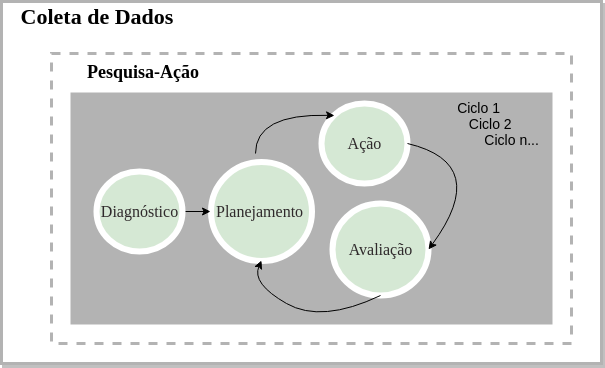
\includegraphics[width=12cm]{figuras/etapasPesquisaAcao.png}
          \caption{Etapas da estratégia de Pesquisa-Ação adotada. (Fonte: Elaborado pela Autora.)}
          \label{fig:etapasPesquisaAcao}

        \end{figure}

É importante ressaltar que a estratégia será empregada em ciclos para a fase de implementação do sistema de recomendação, ou seja, a adaptação da ideia e melhoria da proposta deste trabalho irá permitir uma maior iteração com a equipe de testadores de modo que, de maneira colaborativa, se extraiam mais informações relevantes para a otimização da recomendação realizada pelo sistema.

\subsection{Diagnóstico}

Para a construção do sistema de recomendação um \textit{diagnóstico} foi realizado para a compreensão do objeto de estudo. Para a caracterização do objeto de estudo, apresentado no Capítulo \ref{ch:referencial}, foram realizadas pesquisas quanto a sistemas de recomendação e perfil de testadores, a fim de entender o \textit{background} teórico deste trabalho.

% \del{``afundo'' - vem de afundar; ``a fundo'' - em profundidade}

\subsection{Planejamento, Ação e Validação}

As etapas de pesquisa-ação, \textit{planejamento, ação} e \textit{avaliação} serão levadas em consideração para a construção de instrumentos em ciclos de interação com a equipe. A Figura \ref{fig:etapasPesquisaAcaoAdotas} apresenta a estratégia de Coleta de Dados, ressaltando a Pesquisa-ação e respectivas etapas empregadas.

        \begin{figure}[H]
          \centering
          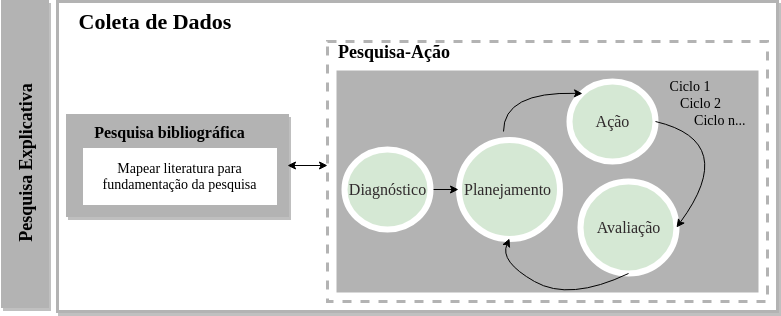
\includegraphics[width=12cm]{figuras/etapasPesquisaAcaoAdotadas.png}
          \caption{Etapas da Pesquisa-Ação adotadas. (Fonte: Elaborado pela Autora.)}
          \label{fig:etapasPesquisaAcaoAdotas}

        \end{figure}

\subsection{Técnicas de Coleta de Dados}

Durante a fase de Coleta de dados foram usadas as técnicas de observação, além de elaboração e uma futura aplicação de questionário para reconhecer o perfil de cada testador. A aplicação do questionário deve ser realizada com duas disciplinas da Universidade de Brasília, Engenharia de Software Experimental e Testes de Software, especificamente.

\section{Análise de Dados}

Após a fase Coleta de Dados, com a aplicação dos procedimentos de coleta de dados definidos, a fase seguinte será a de Análise dos Dados e Resultados, conforme o planejamento da pesquisa e apresentado na Figura \ref{fig:analiseDados}.

        \begin{figure}[H]
          \centering
          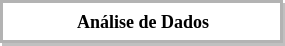
\includegraphics[width=8cm]{figuras/analiseDados.png}
          \caption{Análise de Dados. (Fonte: Elaborado pela Autora.)}
          \label{fig:analiseDados}

        \end{figure}

\section{Resultados}

A fase de resultados corresponde à fase final deste trabalho, na qual os resultados obtidos com a execução do TCC2 serão apresentados. A Figura \ref{fig:resultados} apresenta a última fase do Plano Metodológico.

        \begin{figure}[H]
          \centering
          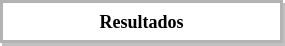
\includegraphics[width=8cm]{figuras/resultados.png}
          \caption{Resultados. (Fonte: Elaborado pela Autora.)}
          \label{fig:resultados}

        \end{figure}


\section{Considerações Finais do Capítulo}

Considerando o foco deste trabalho em definir processos, principalmente, relacionados à atribuição de testes, a metodologia definida surgiu da necessidade de se experimentar um processo de atribuição de casos de testes de acordo com o perfil do testador. Desse modo, neste capítulo, apresentou-se o plano metodológico adotado para se atingir os objetivos desta pesquisa. 

No próximo capítulo apresenta-se a proposta deste trabalho, com as atividades já realizadas e as por realizar. Com especial detalhamento das atividades em cada estágio da Pesquisa-Ação.

% \del{acho que o cronograma está no capítulo seguinte, correto? rever aqui nas considerações finais o que realmente está nesse capítulo e o que será apresentado no próximo}.
\chapter{Proposta do Trabalho}
\label{ch:proposta}

\section{Considerações Iniciais}

// o volume atual de testes feitos pelo ME. 

Dado o objetivo deste trabalho, o presente capítulo retoma o plano metodológico adotado apresentado no Capítulo \ref{ch:metodologia} e apresenta um detalhamento das atividades já realizadas e as atividades a serem realizadas. 

O detalhamento será descrito quanto às fases de \textit{Planejamento da Pesquisa} e da \textit{Coleta de Dados}, que representam os procedimentos e técnicas utilizados para a consolidação da proposta deste trabalho. Finalizando, apresenta-se o cronograma de execução das atividades a serem realizadas para a conclusão do trabalho.

\section{Atribuição de Casos de Teste Baseado no Perfil de Testadores}

A pesquisa bibliográfica realizada colaborou para a construção da proposta deste trabalho de se realizar uma abordagem para atribuição dinâmica de atividades de teste com base no perfil dos testadores envolvidos no time de testes do ITRAC. 

Cada etapa apresentada neste capítulo consolida uma fase da parte prática deste trabalho, que será executada no TCC2. Para se realizar a elicitação, análise e modelagem dos requisitos para o sistema de recomendação, selecionou-se o procedimento de pesquisa-ação para realização das
atividades de forma participativa e interativa entre pesquisador e membros do objeto de estudo.

Sendo assim, para esta pesquisa, relacionam-se e entendem-se as seguintes etapas:

\begin{enumerate}
    \item Identificação e levantamento de características pessoais que podem influenciar o processo de teste de software no contexto apresentado;

    \item Extração de informações sobre as características pessoais de cada testador envolvido no processo de teste;

    \item Acompanhamento do processo de teste de um serviço fictício criado com diferentes características, registrando métricas que viabilizam a análise da adequação entre tours e testadores específicos;

    % \item Acompanhamento do processo de teste de diversos serviços, com diferentes características, registrando métricas que viabilizam a análise da adequação entre tipos de teste e testadores específicos;

    \item Análise dos dados registrados sobre o teste;

    \item Definição de \textit{Sistema de Recomendação} que se baseia no conjunto de dados registrados sobre o teste no serviço fictício para recomendar casos de teste para testadores;

    \item Proposição de uma estratégia de filtragem para ponderar futuras recomendações, levando em consideração a satisfação do testador durante a realização das atividades de teste.
\end{enumerate}


As Seções \ref{sec:caracteristicas_importantes}, \ref{sec:extrair_caracteristicas}, \ref{sec:acompanhar_ciclos} e \ref{sec:analisar_dados} apresentam as técnicas de coleta de dados e relaciona as principais etapas da abordagem proposta neste trabalho.

\section{Características de Perfil}
\label{sec:caracteristicas_importantes}

A técnica de \textit{Observação}, proposta como técnica de coleta de dados em uma das fases da metodologia adotada, foi empregada neste trabalho a partir do estudo sobre a equipe objeto de estudo.

Como já apresentado no Capítulo \ref{ch:referencial}, na Seção \ref{sec:perfil_testadores}, a influência da personalidade humana em tarefas individuais é uma das preocupações da Engenharia de Software.  Sendo assim, a influência da personalidade também é uma característica importante deste trabalho, pois configura o mecanismo principal para realização da Atribuição dos casos de teste dinamicamente.

A equipe de testadores do ITRAC possui membros com níveis variados de experiência em testes, sendo composta por alunos graduandos em Engenharia de Software, que cursam períodos diferentes do curso, podendo variar entre calouros e veteranos. Além disso, parte da equipe que realiza os testes nos serviços, utilizando o processo de testes definido pelo ITRAC, é composta por funcionários do ME, já graduados em diferentes cursos, que podem possuir, ou não, uma maior experiência em testes, de um modo geral.

Esta variação entre os membros da equipe e seus respectivos conhecimentos não é considerada no momento da Atribuição de tarefas de teste realizadas. Sendo assim, alunos que estão no início da graduação e sem nenhuma experiência em testes, podem ser alocados a tarefas de teste que possuem o mesmo nível de dificuldade de tarefas de teste alocadas a testadores experientes.

Esta falta de critério na Atribuição de tarefas de teste pode gerar prejuízos ao processo de Validação do produto de software. Este problema é atacado no trabalho atual, objetivando uma melhor adequação entre os testadores e as tarefas teste realizadas.

\section{Extração de Informações de Perfil}
\label{sec:extrair_caracteristicas}

Neste trabalho, é necessário extrair as informações sobre o perfil de cada testador da equipe do ITRAC. A extração de informações é feita a partir da \textit{técnica de Coleta de Dados Questionário}. O Questionário foi desenvolvido com base em~\cite{Santos19SDPA}, \cite{geras2004survey} e~\cite{groves2000survey} e é apresentado no Anexo~\ref{anexo:questionario}.

A criação do questionário foi baseada nas  diretrizes de Kitchenham~\cite{kitchenham2008personal} que apresenta 6 etapas a serem realizadas, como ilustrado na Figura~\ref{fig:Abordagem}.

        \begin{figure}[h]
          \centering
          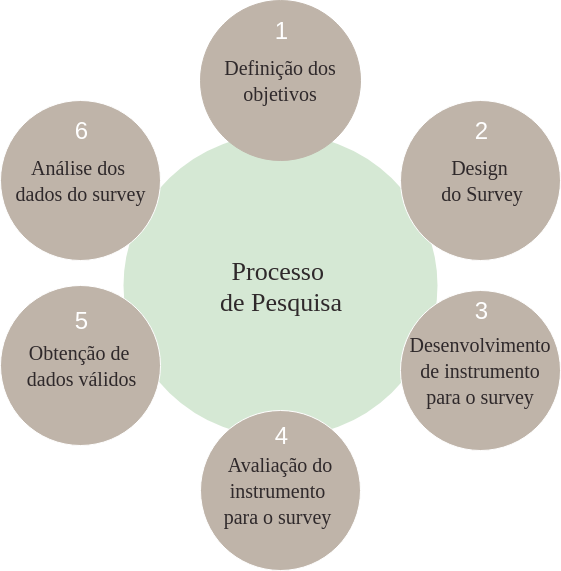
\includegraphics[width=10cm]{figuras/survey.png}
          \caption{Visão geral do processo para elaboração do questionário.  (Fonte: Elaborado pela Autora.)}
          \label{fig:Abordagem}

        \end{figure}

As 6 etapas estão sendo empregadas neste, conforme descrição a seguir:

\begin{enumerate}
\item \textbf{Estabelecer objetivos:} neste trabalho, esta etapa configura o primeiro passo para começar a construir o questionário. Em que cada objetivo é definido;

\item \textbf{Design do \textit{survey}:} o tipo de \textit{design} utilizado neste trabalho é o transversal~\cite{geras2004survey}, no qual os participantes serão questionados sobre suas experiências prévias;

\item \textbf{Desenvolvimento de instrumento para o \textit{survey}:} para desenvolver o instrumento, foram empregados os passos: (i) pesquisar a literatura relevante (apresentada no Capítulo~\ref{ch:referencial}); (ii) construir um instrumento (Capítulo~\ref{ch:metodologia}); (iii) avaliar o instrumento (em produção); e (iv) documentar o instrumento (redação do trabalho como um todo);

\item \textbf{Avaliação do instrumento para o \textit{survey}:} esta avaliação é frequentemente chamada de pré-teste, e possui objetivos distintos: (i) verificar se as questões são compreensíveis; (ii) avaliar a taxa de resposta provável e a eficácia dos procedimentos de acompanhamento; (iii) avaliar a confiabilidade e validade do instrumento; e (iv) garantir que nossa análise de dados as técnicas correspondem às nossas respostas esperadas;

\item \textbf{Obtenção de dados válidos:} nesta fase é definida uma amostra, que é um subconjunto da população. As respostas deste grupo buscam representar o grupo inteiro. Ao escolher a amostra a ser pesquisada, devemos ter em mente três aspectos do desenho da pesquisa: (i) evitar o viés; (ii) adequação; e (iii) custo-efetividade;

\item \textbf{Análise dos dados do \textit{survey}:} na etapa final, são reunidos todos os dados coletados da pesquisa para extrair informações relevantes para responder às questões definidas nos objetivos da pesquisa e descritas no GQM, destacado na Tabela~\ref{tab:gqm}.
\end{enumerate}

Para este trabalho de conclusão de curso (TCC1), foram realizados as 2 primeiras etapas e parte da terceira. O restante das etapas configuram parte do trabalho a ser realizado no TCC2.

\subsection{Design e Questões do Questionário}
\label{sec:desingquestions}

Para projetar o questionário buscou-se na literatura trabalhos similares.

O questionário foi elaborado tomando como base outros artigos que realizavam este tipo de pesquisa, por exemplo, o \textit{survey} de~\cite{geras2004survey}, que descreveu os resultados de um \textit{survey} de questionamentos feitos à pessoas envolvidas com o desenvolvimento de software em uma empresa. A partir disso, com o objetivo de caracterizar testes de software e práticas de garantia da qualidade, o questionário foi dividido nas seguintes categorias:

Exemplo \cite{model1980multiprocessing}

\begin{itemize}
\item  Perfil pessoal e profissional dos respondentes;
\item  Conhecimentos específicos de teste; e
\item  Relato livre de experiência.
\end{itemize}

As perguntas referentes à cada categoria podem ser consultadas no Anexo~\ref{anexo:questionario}.

A primeira categoria foi elaborada com o objetivo de coletar informações pessoais e sobre o perfil profissional do respondente, com o interesse em entender o nível de escolaridade, respectivos cursos de graduação, experiências com linguagens de programação e para coletar os usuários de cada testador na ferramenta de gerenciamento de projetos utilizada. No contexto desta pesquisa, foi utilizada a ferramenta \textit{redmine}\footnote{https://www.redmine.org/}.

A segunda categoria busca entender o grau de familiaridade dos testadores com a atividade de teste. Para isto, o questionário aborda questões sobre técnicas e critérios de teste, por exemplo, para entender como é a experiência dos testadores neste quesito.


A terceira categoria engloba uma questão aberta, que solicita ao testador que relate a sua experiência. Esta questão se faz importante, pois as respostas serão fundamentais para que o testador relate livremente sua experiência, podendo incluir informações que o questionário ainda não contém, mas que são relevantes para a pesquisa. Podendo colaborar, dessa forma, com o aprimoramento do questionário.

É interessante ressaltar que o questionário ainda está em fase de construção e será aprimorado após uma primeira aplicação com um membro do ITRAC, que fará parte da equipe de testes dos serviços.

\section{Acompanhar Ciclos}
\label{sec:acompanhar_ciclos}

Para se utilizar dados necessário para o desenvolvimento do sistema, foi utilizada uma estratégia de registro de informações que envolve 4 etapas propostas por \cite{petersen2008systematic}, apresentada na Subseção~\ref{sub:pesquisa-acao} e ilustrada na Figura~\ref{fig:etapasPesquisaAcaoAdotas}.

        \begin{figure}[!htb]
          \centering
          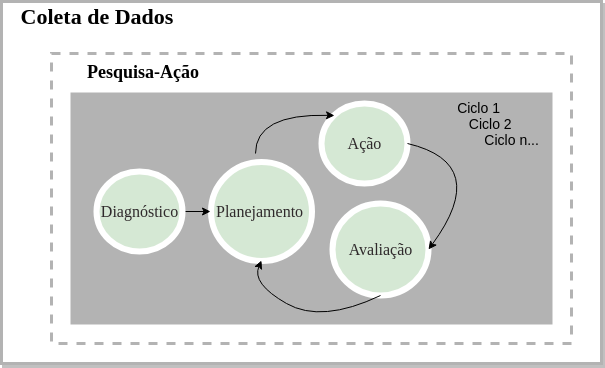
\includegraphics[width=12cm]{figuras/etapasPesquisaAcao.png}
          \caption{Etapas da estratégia de Pesquisa-Ação adotada. (Fonte: Elaborado pela Autora.)}
          \label{fig:etapasPesquisaAcao}

        \end{figure}

Na fase de \textit{Diagnóstico}, buscou-se entender o processo que os testadores seguem para descobrir como seriam feitos os registros de determinadas informações. Estas informações necessárias são apresentadas, também, na Tabela~\ref{tab:gqm}, que será apresentada mais à frente. A partir disso, foi feita a construção de um fluxo, apresentado na Figura~\ref{fig:fluxo}, que deve ser seguido até que se inicie o desenvolvimento do sistema de recomendação.

        \begin{figure}[!htb]
          \centering
          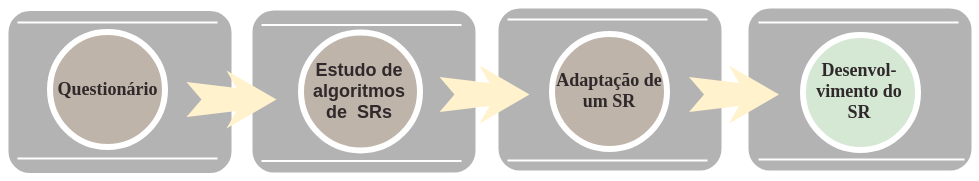
\includegraphics[width=16cm]{figuras/fluxo.png}
          \caption{Fluxo para desenvolvimento do SR.  (Fonte: Elaborado pela Autora.)}
          \label{fig:fluxo}

        \end{figure}

Com o objetivo de facilitar o entendimento das funcionalidades do sistema, apresentar um protótipo e validá-lo com a equipe do ITRAC, serão empregados alguns ciclos. Os ciclos serão desenvolvidos no TCC2.

O acompanhamento de ciclos deve levar em consideração o registro de determinadas informações. Para tanto, foi necessária a elaboração de um \textit{Goal Question Metric - GQM}, que consiste em um mecanismo utilizado para definir e avaliar um conjunto de objetivos operacionais, utilizando um conjunto de questões e métricas associadas a estes objetivos~\cite{basili1994goal}. O GQM desta pesquisa é apresentado na Tabela~\ref{tab:gqm}:

% Please add the following required packages to your document preamble:
% \usepackage[table,xcdraw]{xcolor}
% If you use beamer only pass "xcolor=table" option, i.e. \documentclass[xcolor=table]{beamer}
\begin{table}[htb!]
\caption{\textit{Goal Question Metric} (GQM).}
\label{tab:gqm}
\begin{tabular}{|l|l|}
\hline
\rowcolor[HTML]{C0C0C0}
\textbf{Goal} & \begin{tabular}[c]{@{}l@{}}Aprimorar o gerenciamento de testes para a atribuição de \\ tarefas de teste com base no perfil do testador\end{tabular} \\ \hline
\rowcolor[HTML]{FFFFFF}
\textbf{Question 1} & Qual a eficiência da Atribuição de tarefas de teste para a equipe? \\ \hline
\rowcolor[HTML]{FFFFFF}
\textbf{Métricas} & \begin{tabular}[c]{@{}l@{}}M1: Número de casos de teste gerados pela equipe\\ \\ M2: Número de falhas identificadas pela equipe\\ \\ M3: M2/M1\end{tabular} \\ \hline
\rowcolor[HTML]{EFEFEF}
\textbf{Question 2} & Qual a eficiência da Atribuição de casos de teste por parte do testador? \\ \hline
\rowcolor[HTML]{EFEFEF}
\textbf{Métricas} & \begin{tabular}[c]{@{}l@{}}M1: Número de casos de teste gerados pelo testador\\ 		\\ M4: Número de falhas identificadas por testador\\ 		\\ M5: M4/M3\end{tabular} \\ \hline
\rowcolor[HTML]{FFFFFF}
\textbf{Question 3} & Qual o impacto do perfil do testador na eficiência dos testes? \\ \hline
\rowcolor[HTML]{FFFFFF}
\textbf{Métrica} & M5: Variação entre a eficiência de cada testador \\ \hline
\rowcolor[HTML]{EFEFEF}
\textbf{Question 4} & Qual o grau de satisfação do testador durante o ciclo de teste? \\ \hline
\rowcolor[HTML]{EFEFEF}
\textbf{Métrica} & M6: Grau de satisfação (0 a 5) \\ \hline
\rowcolor[HTML]{FFFFFF}
\textbf{Question 5} & Qual a eficiência dos testes em relação a cada tour? \\ \hline
\rowcolor[HTML]{FFFFFF}
\textbf{Métrica} & M6 (tour 1) = M1(tour 1)/M4(tour1) \\ \hline
\end{tabular}
\end{table}

Dadas as etapas destacadas, a Seção~\ref{sec:abordagem} apresenta a abordagem proposta neste trabalho.

\section{Abordagem}
\label{sec:abordagem}

A abordagem proposta nesta pesquisa envolve um processo contínuo de aprendizado e evolução, que depende de diversos ciclos de teste em diferentes tipos de serviço. O contexto no qual o laboratório ITRAC se encontra viabiliza a aplicação de tal abordagem, dada as características de um processo de transformação digital em grande escala.

O processo de transformação digital do governo brasileiro envolve um grande número de serviços de baixa complexidade, o que possibilita um grande número de ciclos de teste em um curto período de tempo. Tal característica favorece o aprendizado e a evolução relacionada as atividades de teste neste contexto.

A partir das métricas destacadas na Tabela~\ref{tab:gqm}, é possível que análises sejam realizadas buscando uma melhora contínua da atividade de Atribuição de casos de teste.

Neste sentido, a Figura~\ref{fig:Abordagem} apresenta o processo contínuo de aprendizado, juntamente com a abordagem proposta para este trabalho. Foi utilizado o \textit{lemniscate} -- figura do número 8 virada para representar o processo.

        \begin{figure}[h]
          \centering
          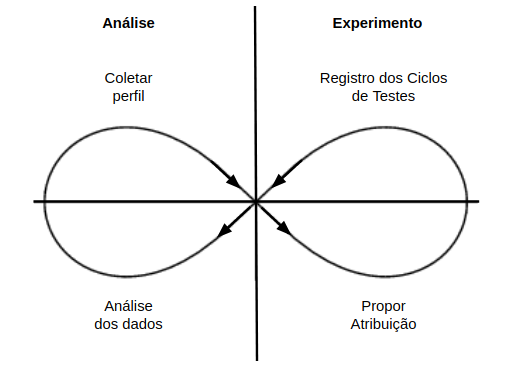
\includegraphics[width=13cm]{figuras/abordagem.png}
          \caption{Abordagem para o Sistema de Recomendação  (Fonte: Elaborado pela Autora.)}
          \label{fig:Abordagem}

        \end{figure}


A parte esquerda da figura relaciona-se com a Análise e está vinculada à coleta do perfil do testador e à análise dos dados coletados depois de cada ciclo de teste. Enquanto a parte direita relaciona o que se pretende usar como experimento, que configura o registro dos ciclos de teste e a proposta de Atribuição. A seguir, serão descritas cada fase da abordagem:

\subsection{Coletar Perfil}

% Perfil será coletado a partir dos alunos das disciplinas de Testes de Software e de Software Experimental

Como apresentado na Seção~\ref{sec:caracteristicas_importantes}, as características de perfil de cada testador serão levadas em consideração para a constituição deste trabalho. Para dar início às partes práticas será necessário coletar o perfil dos testadores envolvidos. O perfil de cada testador será traçado a partir da extração de informações do perfil obtidas a partir do questionário já apresentado na Seção \ref{sec:extrair_caracteristicas}.

O questionário será refinado até estabelecer as questões necessárias para consolidar um perfil que contenha as informações necessárias do usuário sobre cada categoria apresentada na Subseção \ref{sec:desingquestions}. Após a consolidação deste perfil, uma página de perfil para cada testador será criada na ferramenta \itractool para que os testadores tenham um cadastro com todas as informações coletadas.

\subsubsection{Cadastrar perfil na ferramenta \itractool}

É importante que os testadores tenham seus perfis individuais cadastrados na ferramenta, pois estes perfis irão fornecer a informação sobre o domínio dos testadores sobre testes. Estas informações serão registradas no banco de dados e serão atualizadas de acordo com a realização dos cilos de teste.

Com as informações cadastradas será possível traçar, baseado em dados históricos, qual a tarefa de teste ou o \textit{tour} mais adequado para cada perfil de testador, levando em consideração a experiência do testador com o teste exploratório dos serviços. A partir disso, será possível predizer quais atividades de teste ele está executando com mais eficiência para poder realizar uma melhor Atribuição de atividades de teste. O perfil ideal para o testador seria aquele que conseguisse captar além das características técnicas, a experiência naquele domínio de aplicação para, em seguida, propor uma Atribuição.

\subsection{Propor Atribuição}

 Esta fase consiste na proposta de Atribuição baseada em perfil, ou seja, uma página de um serviço com determinados campos e características específicas pode ter um caso de teste e um testador ideal. O sistema de recomendação sugere quais \textit{tours} são adequados para determinado testador utilizar baseado em seu histórico de testes já realizados. A partir disso, a página e campos em questão são testados.

 Os sistemas de recomendação, como já explicitado no Capítulo \ref{ch:referencial}, na Seção \ref{sec:sistemas}, realizam filtragens de informações que recomendam itens aos usuários. No caso deste trabalho o item é uma Atribuição de \textit{tours} para um testador.

É importante destacar que a execução de um \textit{tour} por parte de um testador, dá origem a um conjunto de teste, gerado a partir do \textit{tour}. A Atribuição de \textit{tours} e testadores deve ser realizada de maneira dinâmica, com um processo de aprendizado durante cada ciclo de teste. Ou seja, a Atribuição dos \textit{tours} e dos testadores deve levar em consideração, além das características já citadas, o aprendizado obtido ao longo dos ciclos de teste anteriores. O aprendizado citado busca maximizar a eficiência da aplicação dos casos de teste. Neste contexto, a palavra ``eficiência'' faz referência a taxa de identificação de falhas durante a aplicação dos casos de teste. Desse modo, a ``eficiência'' é dada pela Equação \ref{eq:eficiencia}.

 \begin{equation}
 \label{eq:eficiencia}
    eficiência = \frac{numero \ de \ falhas\ identificadas}{numero\ de\ casos\ de\ teste\ do\ tour}
 \end{equation}


% \del{Aqui achei que ficou um pouco estranho. Acho que para clarear, precisava falar que, a execução de um tour por parte de um testador, dá origem a um conjunto de teste, gerado a partir do tour. Ai dá para entender que há uma relacionamento entre caso de teste, tour e testador.}

Neste trabalho, assim como proposto em~\cite{miranda2012recommender}, a Atribuição é representada como um par conjunto de teste e testador, representado por \{CTn;Tn\} (Caso de Teste \emph{n} e Testador \emph{n}). O usuário é representado por um típico gerente de teste e as recomendações são feitas comparando um caso de teste específico com o perfil de um testador e avaliando sua similaridade.

Após a Atribuição e a realização dos casos de teste alocados, surge a etapa de registro dos casos de teste, detalhada a seguir.

\section{Registro dos Ciclos de Teste}

Os casos de teste realizados pelos testadores do ITRAC já são registrados na ferramenta \textit{Redmine}. Estes casos de teste já possuem um padrão a ser seguido para terem suas informações guardadas. Com isso, a obtenção dos casos de teste realizados pode ser feita a partir da API (\textit{Application Programming Interface}) do \textit{Redmine}.

A Figura \ref{fig:registro} apresenta a estrutura organizacional atual dos registros realizados no \textit{Redmine}.


        \begin{figure}[h]
          \centering
          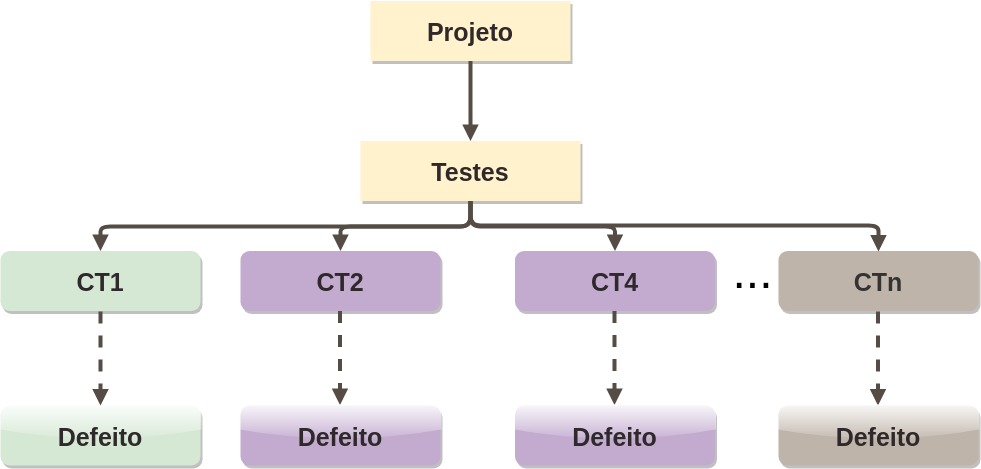
\includegraphics[width=15cm]{figuras/registro.png}
          \caption{Estrutura Organizacional dos Registros no \textit{Redmine}. (Fonte: Elaborado pela Autora.)}
          \label{fig:registro}

        \end{figure}

Na Figura \ref{fig:registro}, \textbf{Projeto} representa um serviço digitizado, que foi registrado no \textit{Redmine}. \textbf{Testes} representam o conjunto de casos de teste associados ao projeto. O conjunto de testes é definido à partir do conceito de \textit{tasks} do \textit{Redmine}. A definição desta entidade que agrupa os casos de teste se deu para facilitar a obtenção de informações de maneira agrupada, viabilizando, por exemplo, a extração do status de conclusão do conjunto de casos de teste como um todo.

Os \textbf{CTs} representam os casos de teste registrados no \textit{Redmine}. Estes são definidos a partir do conceito de \textit{subtasks} associados à \textit{task} \textbf{Testes} e possuem os atributos apresentados na Tabela \ref{tab:atributo}.

% Please add the following required packages to your document preamble:
% \usepackage[table,xcdraw]{xcolor}
% If you use beamer only pass "xcolor=table" option, i.e. \documentclass[xcolor=table]{beamer}
\begin{table}[H]
\centering
\caption{Atributos dos Casos de Teste Registrados no \textit{Redmine}.}
\label{tab:atributo}
\begin{tabular}{|l|l|}
\hline
\textbf{Atributo} & \textbf{Descrição} \\ \hline
Título & Registra o título do caso de teste \\ \hline
\rowcolor[HTML]{EFEFEF}
Data de criação & Registra a data de criação do teste \\ \hline
Data de execução & Registra a data da execução do teste \\ \hline
\rowcolor[HTML]{EFEFEF}
Tempo para execução & \begin{tabular}[c]{@{}l@{}}Registra o tempo gasto para realizar \\ o caso de teste\end{tabular} \\ \hline
Tour utilizada & Registra a tour utilizada para o caso de teste \\ \hline
\rowcolor[HTML]{EFEFEF}
\begin{tabular}[c]{@{}l@{}}Quantidade de \\ campos envolvidos\end{tabular} & \begin{tabular}[c]{@{}l@{}}Registra quantos campos estão envolvidos\\  no caso de teste\end{tabular} \\ \hline
Testador responsável & \begin{tabular}[c]{@{}l@{}}Registra o testador responsável pela execução\\ do caso de teste\end{tabular} \\ \hline
\rowcolor[HTML]{EFEFEF}
Resultado & \begin{tabular}[c]{@{}l@{}}Registra o resultado final da execução do\\ caso de teste (sucesso, ou falha)\end{tabular} \\ \hline
Entrada & Registra as entradas aplicadas ao caso de teste \\ \hline
\rowcolor[HTML]{EFEFEF}
Saída esperada & Registra a saída esperada para o caso de teste \\ \hline
Saída obtida & \begin{tabular}[c]{@{}l@{}}Registra a saída obtida durante a aplicação\\ do caso de teste\end{tabular} \\ \hline
\rowcolor[HTML]{EFEFEF}
Descrição & Registra a descrição do caso de teste \\ \hline
\end{tabular}
\end{table}

Os \textbf{Defeitos} são definidos como \textit{subtasks} das \textit{subtasks} \textbf{CTs} e possuem os atributos apresentados na Tabela \ref{tab:defeito}. Vale ressaltar que os \textbf{CTs} podem possuir, ou não, um \textbf{Defeito} associado. Essa possibilidade de ter ou não um Defeito associado é representado, na Figura \ref{fig:registro}, a partir da utilização de setas trastejadas.

% Please add the following required packages to your document preamble:
% \usepackage[table,xcdraw]{xcolor}
% If you use beamer only pass "xcolor=table" option, i.e. \documentclass[xcolor=table]{beamer}
\begin{table}[H]
\centering
\caption{Atributos dos Defeitos Registrados no \textit{Redmine}.}
\label{tab:defeito}
\begin{tabular}{|l|l|}
\hline
\textbf{Atributo} & \textbf{Descrição} \\ \hline
\rowcolor[HTML]{FFFFFF}
Título & Registra o título do defeito \\ \hline
\rowcolor[HTML]{EFEFEF}
Prioridade & Registra o nível de prioridade para a resolução do defeito \\ \hline
\rowcolor[HTML]{FFFFFF}
Categoria & Registra a categoria a qual o defeito pertence \\ \hline
\rowcolor[HTML]{EFEFEF}
Tipo de falha & Registra o tipo de falha encontrada \\ \hline
\rowcolor[HTML]{FFFFFF}
\begin{tabular}[c]{@{}l@{}}Passos para \\ reproduzir o bug\end{tabular} & Registra os passos que levaram à ocorrência da falha \\ \hline
\rowcolor[HTML]{EFEFEF}
Provas visuais & \begin{tabular}[c]{@{}l@{}}Registra os defeitos encontrados, geralmente, em forma \\ de \textit{prints}, como prova visual\end{tabular} \\ \hline
\rowcolor[HTML]{FFFFFF}
Ambiente & \begin{tabular}[c]{@{}l@{}}Registra em qual sistema operacional, resolução da tela,\\ browser e nível de zoom o a falha ocorreu\end{tabular} \\ \hline
\end{tabular}
\end{table}

Em relação ao atributo \textbf{Tipo de Falha}, vale destacar que os tipos definidos até o momento são: 1) Regra de Negócio, 2) Interface e 3) Validação de Campos.

\section{Análise dos Dados}
\label{sec:analisar_dados}

Com base na análise do GQM, a intenção é verificar a existência de uma correlação entre a eficiência no processo de teste e as diferentes variáveis que compõem o perfil dos testadores. Este perfil será identificado com base em diferentes questões respondidas pelos testadores num questionário digital, como o apresentado no Anexo~\ref{anexo:questionario}.

Ao obter as questões respondidas do questionário, o passo seguinte é coletar os dados sobre a eficiência de cada testador na realização das atividades de teste. Para que se colete estes dados, é possível a realização de testes de correlação para identificar se há alguma relação entre as variáveis do perfil e a eficiência nos testes de determinado testador ou da equipe de testes como um todo.

Baseado nos dados, pode-se retomar à pergunta de pesquisa e entender: \textbf{Qual o impacto das variáveis do perfil do testador na eficiência dos testes?} A partir desta fase, é possível utilizar o questionário para fazer um teste de correlação entre as variáveis levantadas.


\section{Integração \itractool}

Este trabalho propõe a inclusão de um novo módulo na ferramenta \itractool, apresentada na Seção \ref{sec:dtest}. A integração deste módulo segue o apresentado na Figura \ref{img:architecture2}.

\begin{figure}[!htb]
  \centering
  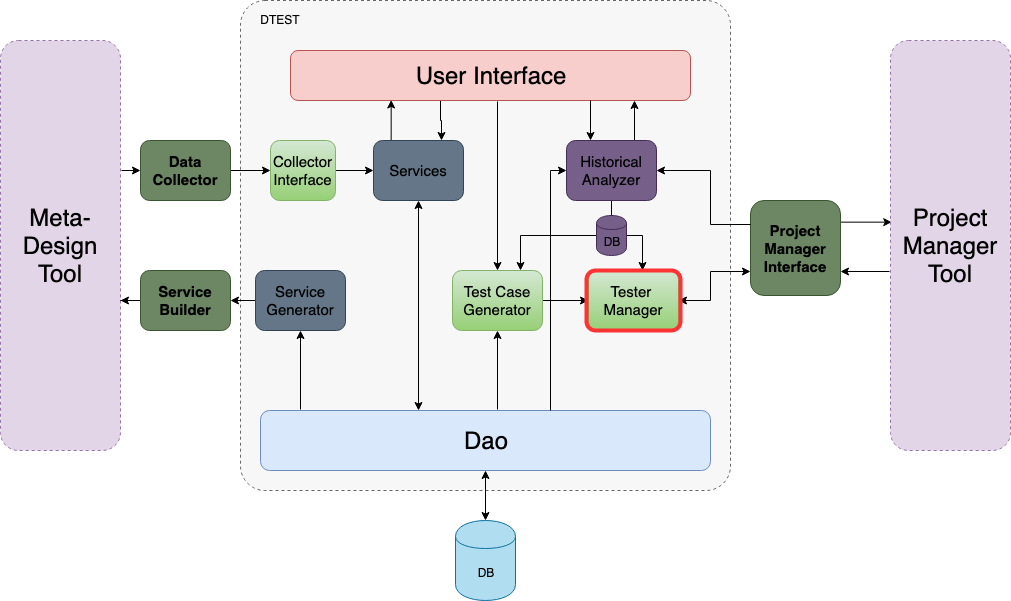
\includegraphics[width=14cm]{figuras/arquitetura.png}
  \caption{Arquitetura \itractool após a inclusão do módulo \textit{Tester Manager}.)}
  \label{img:architecture2}
\end{figure}

O módulo proposto, chamado de \textbf{Tester Manager}, utiliza como \textit{input} informações advindas dos módulos \textbf{Test Case Generator} (TCG) e \textbf{Historical Analyzer} (HA), além de informações diretamente obtidas a partir da ferramenta de gerenciamento de projetos utilizada.

O módulo TCG exporta o caso de teste que deverá ser alocado entre os testadores disponíveis. O módulo \textbf{Tester Manager}, com base nas informações de perfil de cada testador, deverá associar o testador que mais se adéqua ao caso de teste em questão. Para isso, informações histórias da execução de casos de teste são utilizadas como base de conhecimento. Um processo de aprendizado utilizando esta base de conhecimento viabiliza a implementação de um \textit{Sistema de Recomendação} que seja capaz de recomendar o testador mais adequado para determinado caso de teste.


\section{Cronograma}

A Figura \ref{fig:cronograma} apresenta o cronograma de atividades do Trabalho de conclusão de Curso. Desde as atividades já realizadas durante o TCC1 até a concretização do sistema de recomendação, prevista para ser desenvolvida no TCC2.

Na Figura \ref{fig:cronograma}, a cor destacada em verde representa as atividades já desenvolvidas, considerando o término do TCC 1. Em amarelo, as atividades a serem desenvolvidas.

        \begin{figure}[H]
          \centering
          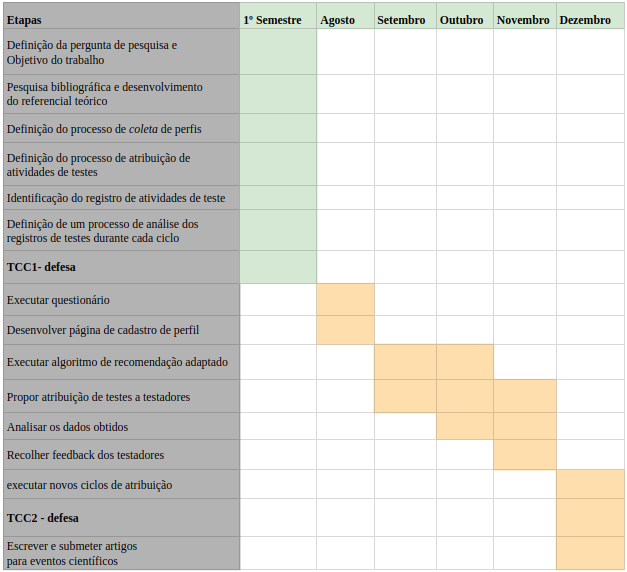
\includegraphics[width=15cm]{figuras/cronograma.png}
          \caption{Cronograma (Fonte: Elaborado pela Autora.)}
          \label{fig:cronograma}

        \end{figure}

\section{Considerações Finais do Capítulo}
\label{sec:final-cap}

Analisando o contexto no qual o ITRAC está inserido é possível perceber um ambiente propício para a aplicação da abordagem proposta, visto que já existe uma ferramenta sobre testes em desenvolvimento. A integração de um módulo que proponha a atribuição dos casos de teste é viável nesta equipe se considerarmos as informações obtidas a partir da ferramenta.

Enquanto os demais capítulos sintetizaram o \textit{background} para a realização deste trabalho, o presente capítulo buscou apresentar a abordagem proposta para este trabalho. Detalhada e apresentada em modelo e de arquitetural. 

Espera-se que no TCC2 o desenvolvimento desta ferramenta seja concretizado e colocado em uso para os testadores do ITRAC. 

\chapter{Resultados}
\label{ch:resultados}

\section{Experimentos com a Ferramenta de Transformação Digital}

\subsection{Ameaça à Validade}

A estratégia inicial para a coleta das informações sobre o perfil dos testadores, foi traçada para ser realizada a partir da execução da proposta deste trabalho com a equipe de testadores do Ministério da Economia. Entretanto, devido a um impasse entre 

\bookmarksetup{startatroot} 

\postextual

\bibliography{bibliografia} 
\begin{anexosenv}
\partanexos

\chapter{Questionário para Extração de Perfil}\label{anexo:questionario}

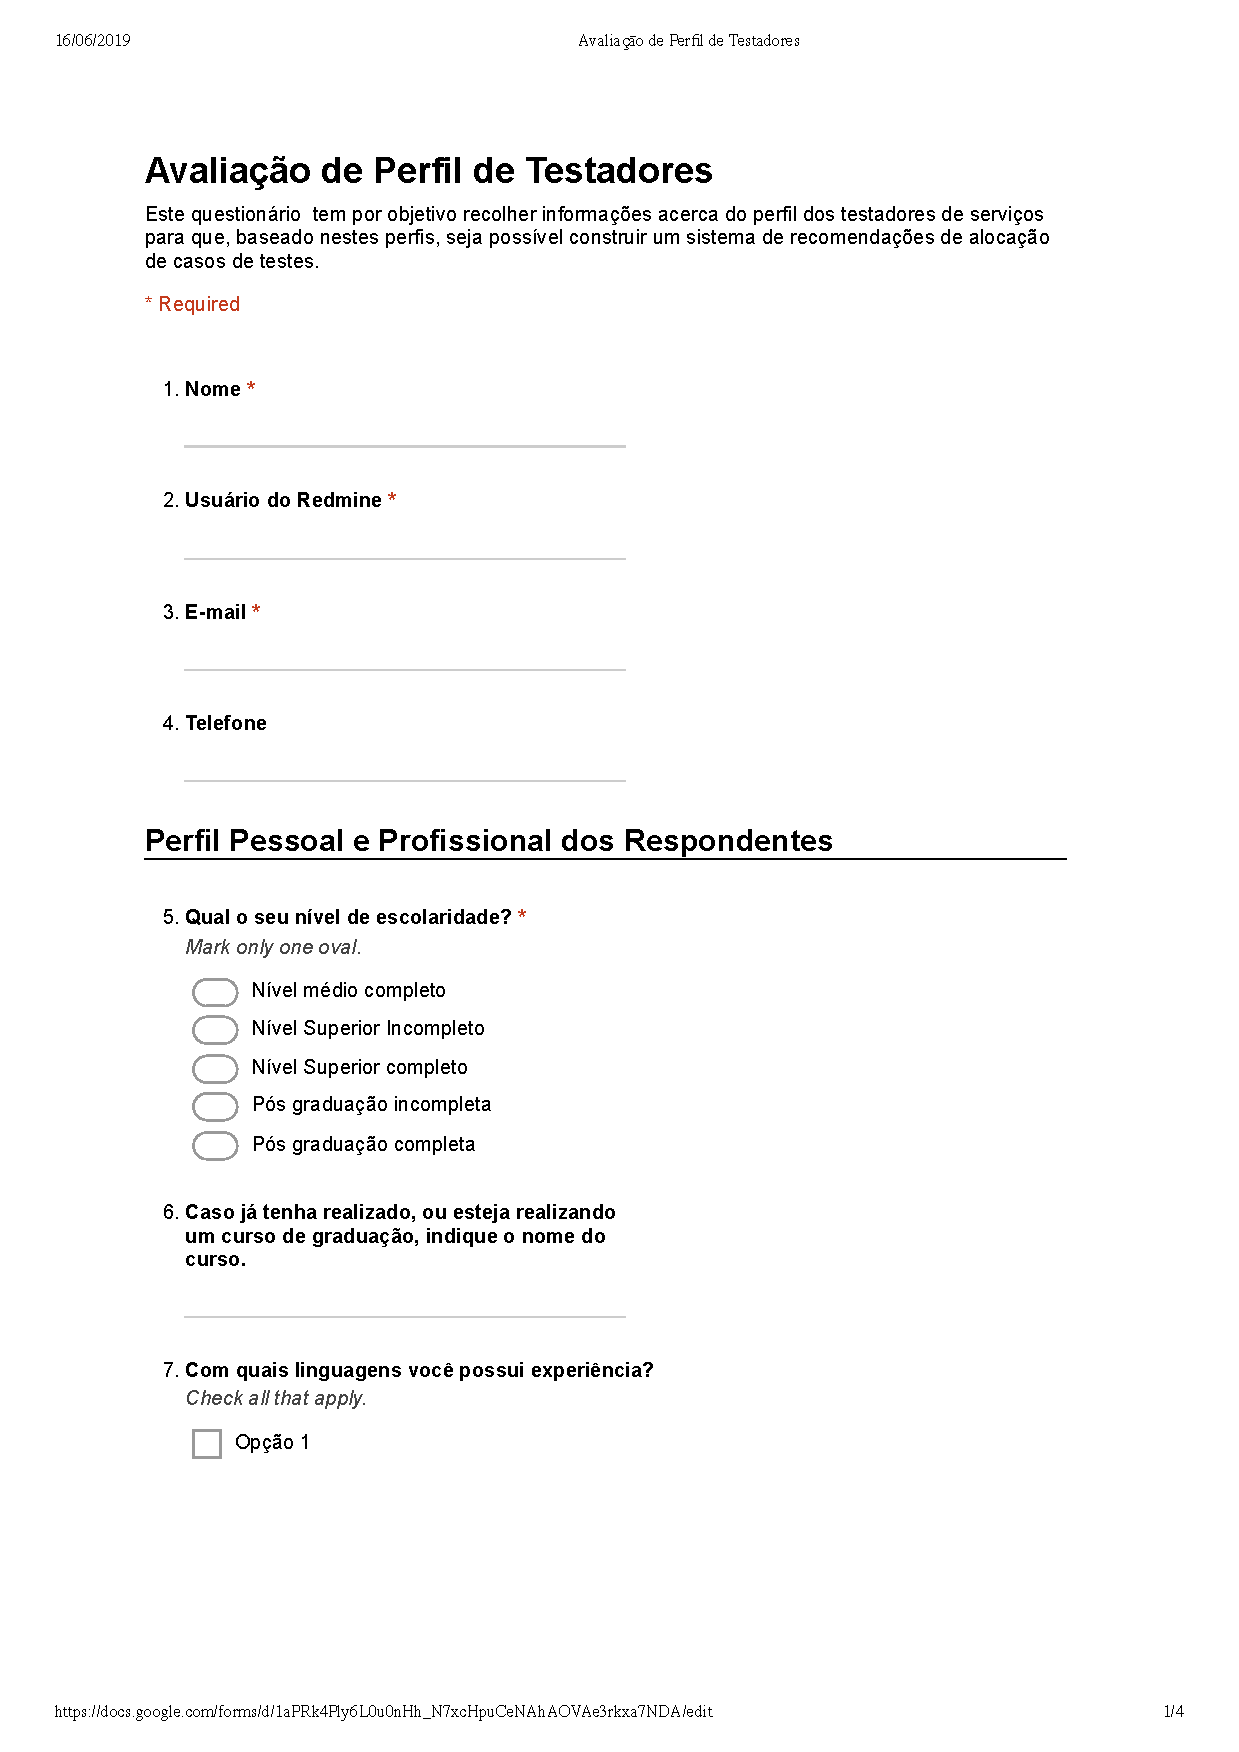
\includepdf[pages=-]{figuras/avaliacao_perfil.pdf}

\chapter{Guia para Aplicação de Testes Exploratórios, Utilizando a Metáfora do Turista, em uma Ferramenta de Transformação Digital}\label{anexo:guiaTestesExploratorios}

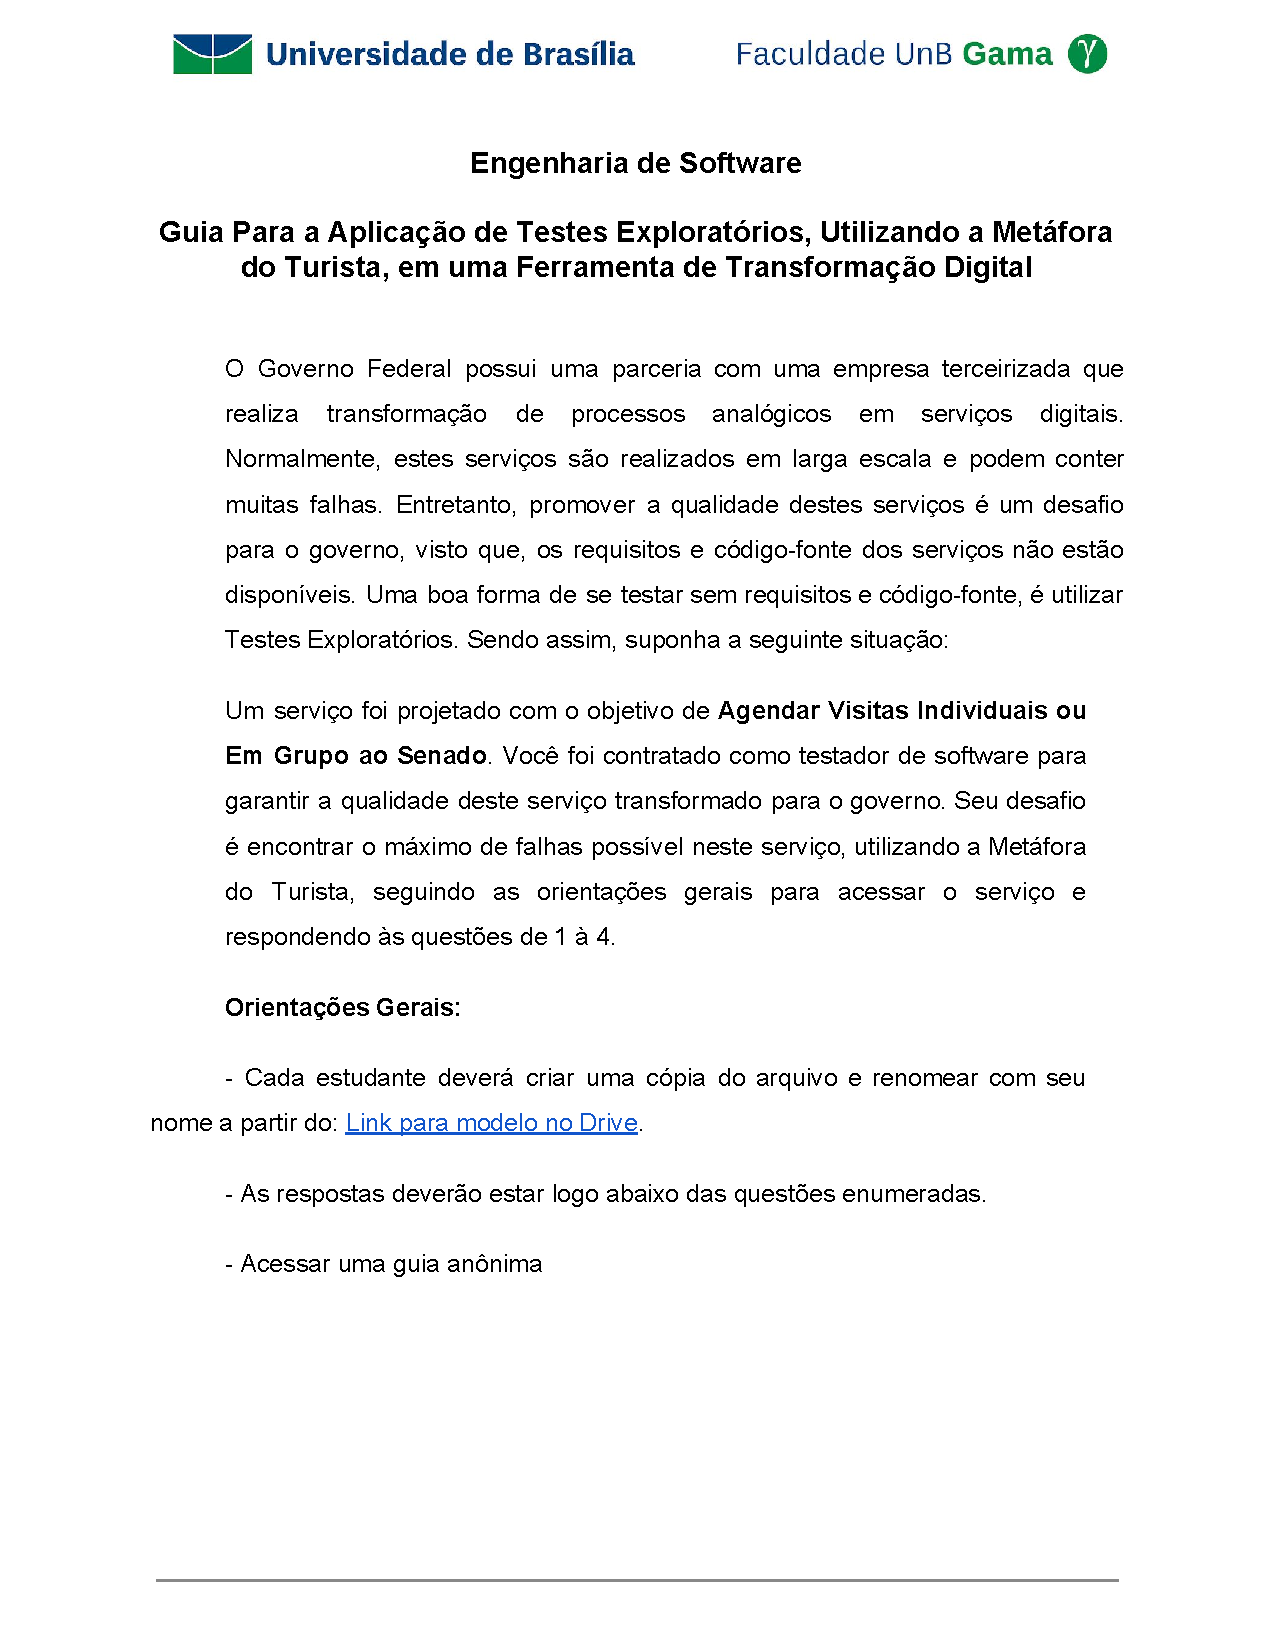
\includepdf[pages=-]{figuras/GuiaTesteExploratorio.pdf}

\chapter{Serviço Fictício}\label{anexo:servicoFicticio}

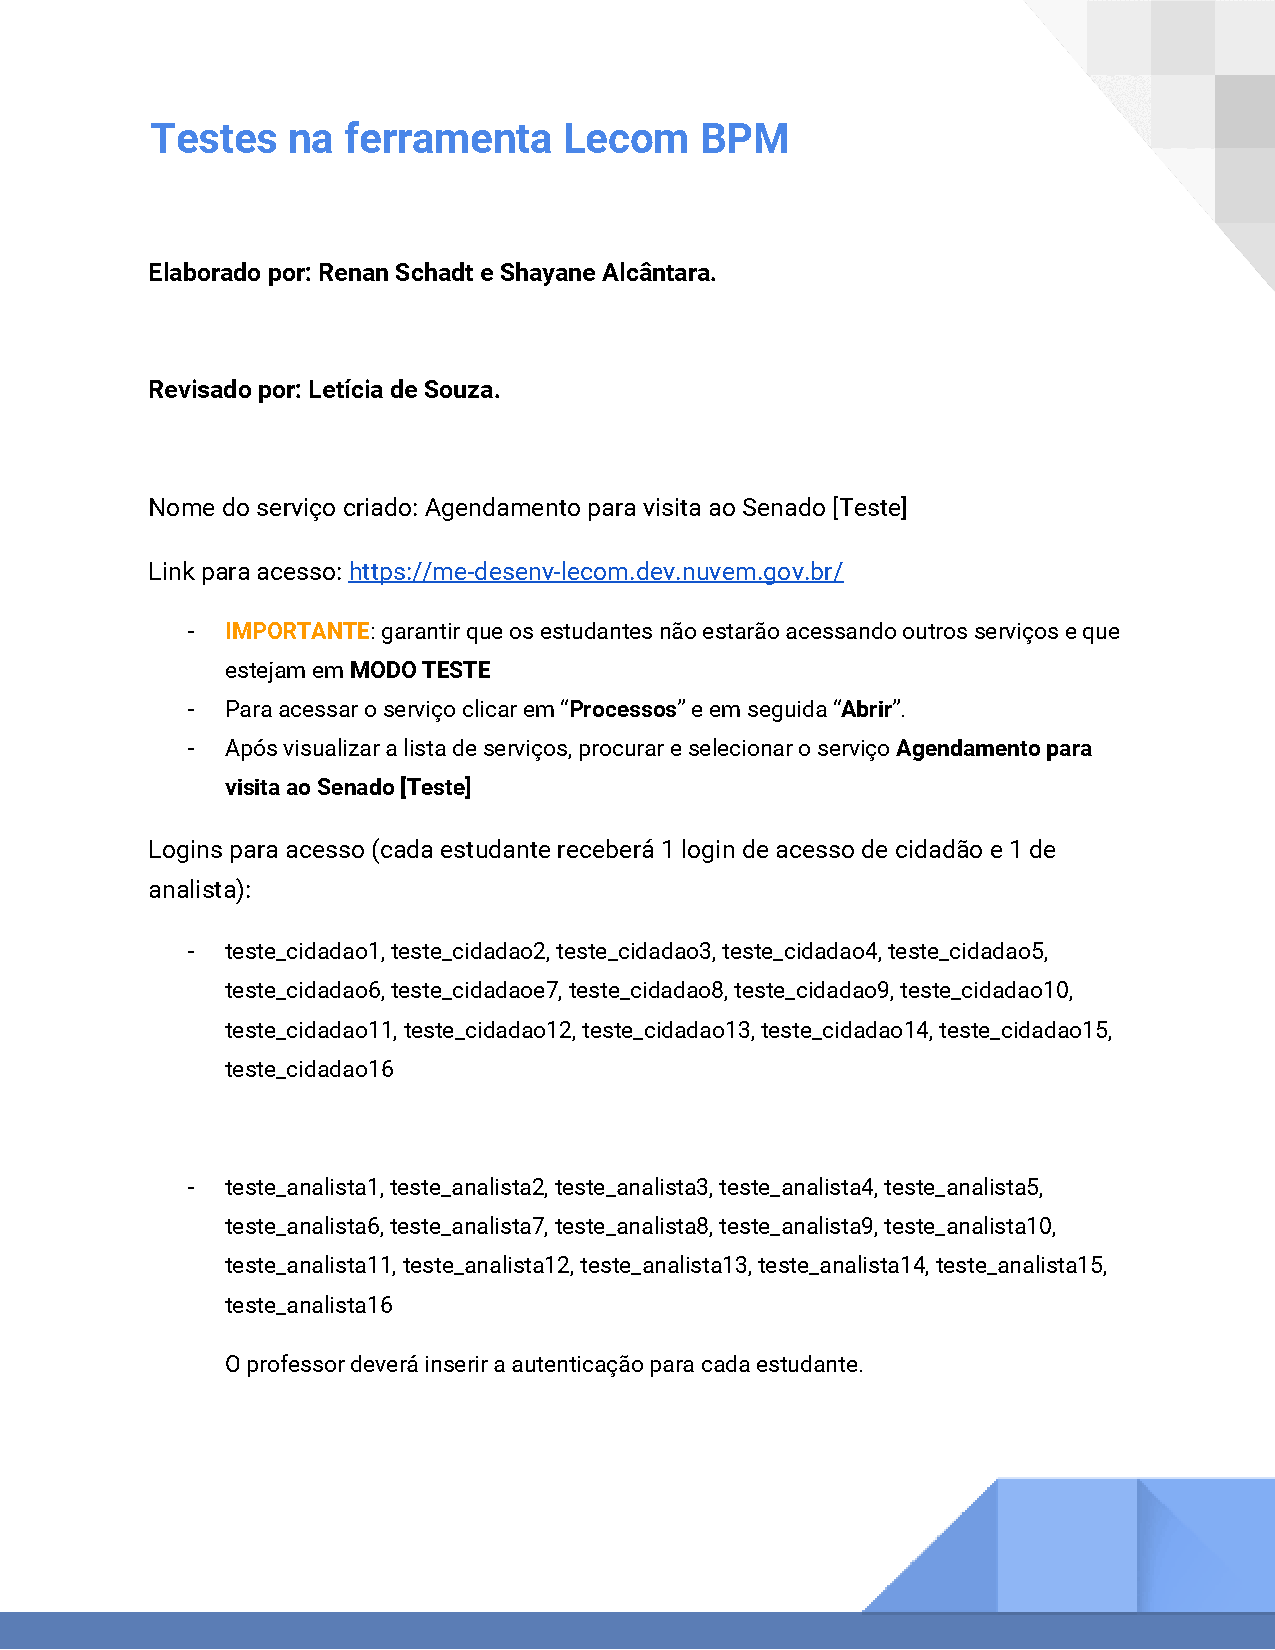
\includepdf[pages=-]{figuras/servicoFicticio.pdf}

\chapter{Resumo sobre Testes Exploratórios de Escopo Abrangente - Metáfora do Turista}\label{anexo:resumoTours}

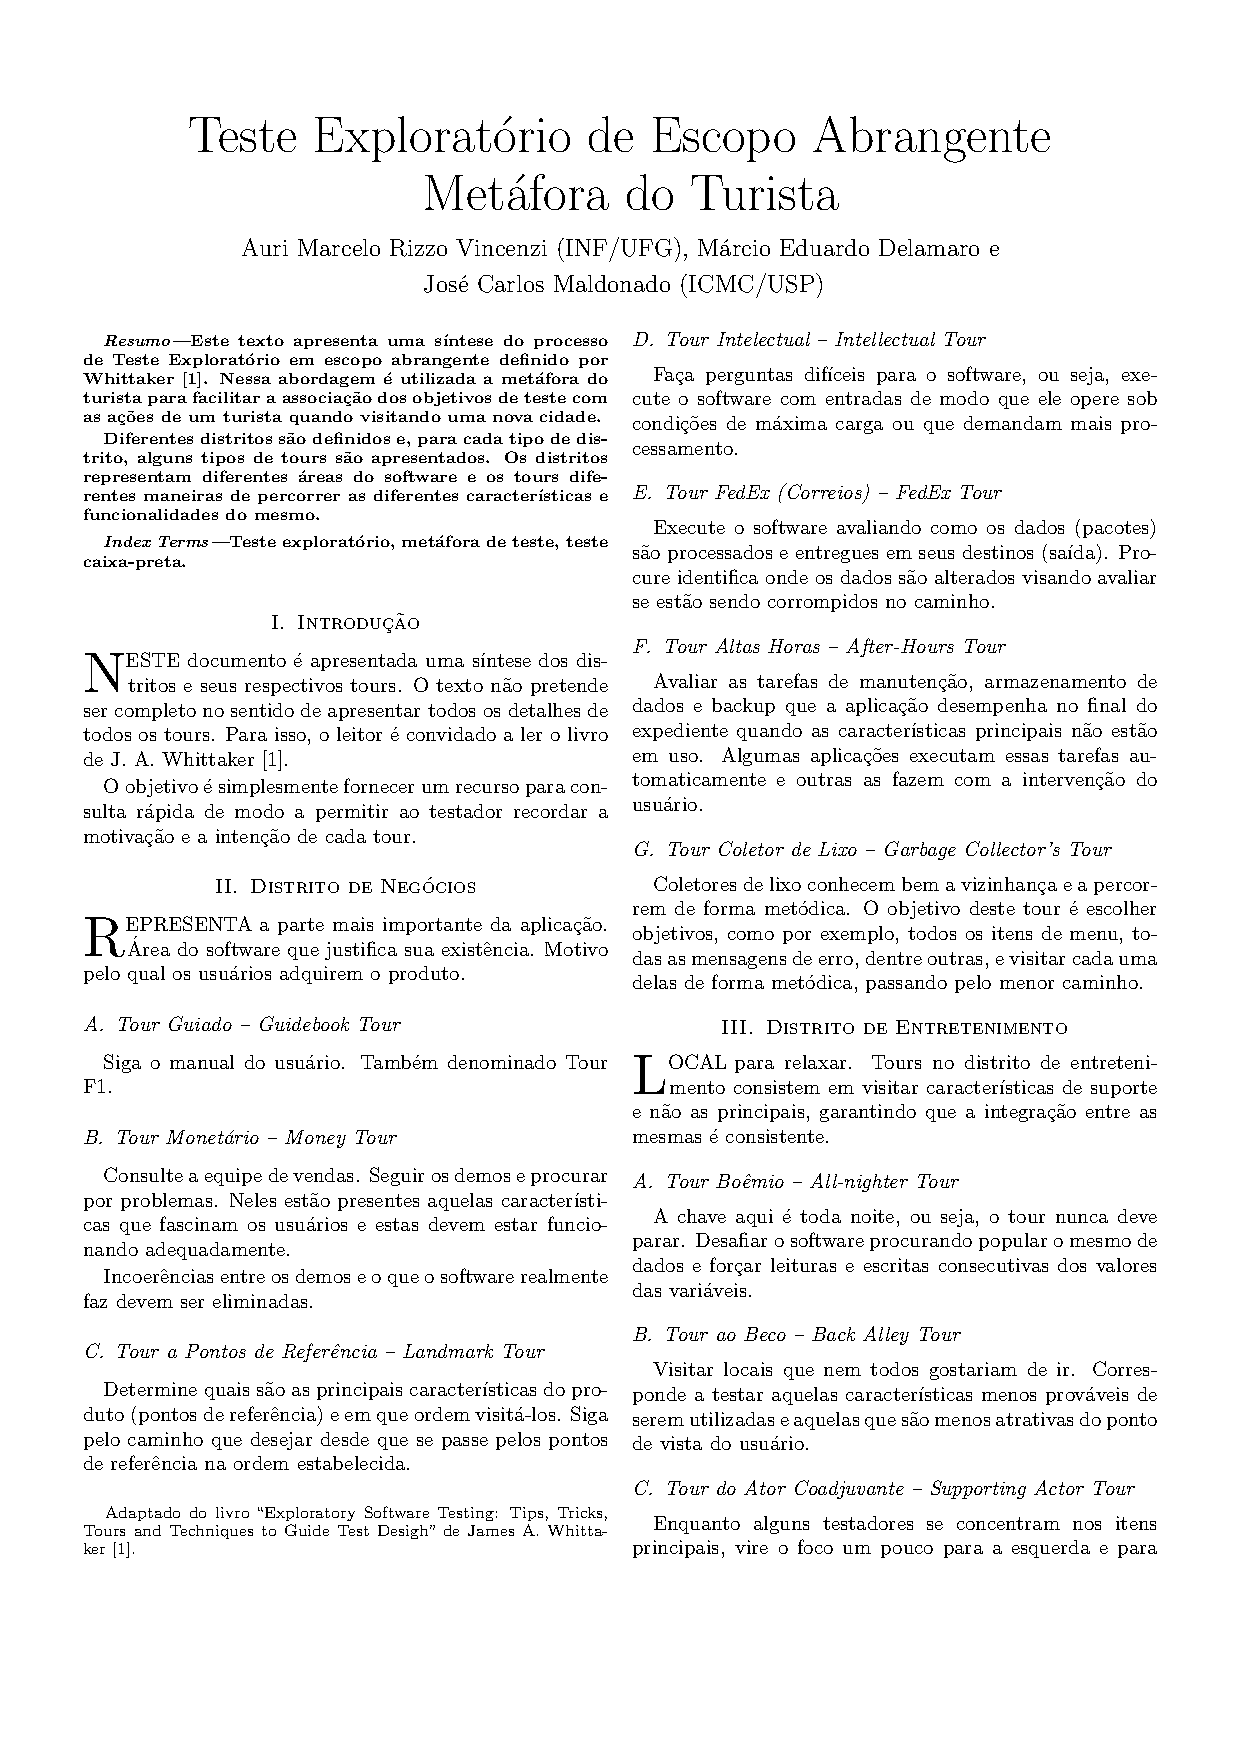
\includepdf[pages=-]{figuras/resumo-tours.pdf}


\end{anexosenv}


\printindex

\end{document}

